% Author: Otakar Kočí 2025-2026 

%%%%%%%%%%%%%%%%%%%%%%%%%%%%%%
% Introduction
%%%%%%%%%%%%%%%%%%%%%%%%%%%%%%
\chapter{Introduction}\label{introduction}


Procedural content generation (PCG) techniques are increasingly used in game development and in games themselves. At the same time, some games require voxel environments to implement their gameplay features. This is especially true in the growing market of sandbox voxel games, such as Minecraft and the recently released Hytale, which heavily use both approaches.

This thesis aims to study the use of procedural generation methods and voxel environments in games. Most importantly, it aims to design a~procedural world generator of voxel game maps focused on natural landscapes and implement it in a~voxel game demo. 

The result of this thesis is a~fully procedurally generated sandbox voxel game demo that supports exploration and basic editing of vast, pseudo-infinite worlds with high voxel detail. It creates naturally inspired voxel environments, featuring diverse and dynamic terrain with mountains, valleys, and plateaus, as well as underground cave systems. The world's surface features water elements such as lakes and rivers that follow terrain properties, together with biomes that are based on realistic attributes such as terrain height and water availability, and form diverse environments with vegetation and decorations. These environments range from snow-covered mountains, through arid plains and deserts, to meadows and forests with lush vegetation. The demo uses the Godot Engine and is implemented in C\#. The engine is used only for rendering, physics, input abstraction, and user interfaces. All other aspects of the demo, including voxel management, world generation pipeline, chunk system, geometry extraction with support for levels of detail, and more, are implemented as part of this thesis. The centerpiece of the implementation is a~custom hierarchical chunk system with multiple layers, which uses distributed tasks for the generation, visualization, and unloading of world segments and is heavily parallelized. The demo also supports multiple worlds, configurable world generation, rendering settings, and more.

This thesis begins with an introduction to the use of procedural generation and voxel environments in games in Chapter~\ref{intro-game-dev-proc-gen}. Chapter~\ref{proc-gen-methods} follows with a~study of a~set of important PCG methods, and Chapter~\ref{tech-sol-voxel-worlds} studies technical aspects of voxel representation. Then follows the design of a~procedural world generator in Chapter~\ref{world-gen-design}, and its implementation in a~pseudo-infinite sandbox voxel game is described in Chapter~\ref{implementation}. Finally, the results are analyzed in Chapter~\ref{testing-showcase}.



%%%%%%%%%%%%%%%%%%%%%%%%%%%%%%
% Game Dev, Proc Gen, Voxel Intro
%%%%%%%%%%%%%%%%%%%%%%%%%%%%%%
\chapter{Procedural Content Generation and Voxel Environments in Games}\label{intro-game-dev-proc-gen}

This chapter provides an introduction to the use of procedural content generation (PCG) and voxel environments for game development. Reasons for using such methods and representations are covered, along with their drawbacks. Various tools and game engines for developing procedural and voxel games are discussed, and games that utilize these approaches are showcased.

\section{Game Development with PCG and Voxels}

Modern games are becoming increasingly complex, requiring larger development teams and larger budgets~\cite{proc_gen_survey_mdpi, procdural_generation_game_design_book, proc_gen_review}. This and more reasons, such as the ability to reduce the installation sizes of games, or the possibility to utilize PCG techniques to create never-ending games with seemingly infinite amounts of content or world space, promote the use of PCG methods and accelerate their adoption in both the development of modern games and their use in games themselves. At the same time, many games feature gameplay mechanics that require voxel representation.

\subsection{Procedural Content Generation in Games}

Procedural content generation~\cite{proc_gen_review, proc_gen_survey_mdpi, proc-cont-gen-games-survey-hendrikx, procdural_generation_game_design_book} is a~large set of methods, algorithms, and approaches that can be used to automatically generate or alter game content. A~bit broader definition from a~PCG survey follows:

\begin{quote}
    Procedural content generation is the automatic creation of digital assets for games, simulations, or movies based on predefined algorithms and patterns that require minimal user input~\cite{proc_gen_survey_mdpi}.
\end{quote}

Generally, PCG can be used to generate~\cite{proc-cont-gen-games-survey-hendrikx, proc_gen_review, procdural_generation_game_design_book} game assets (3D objects, textures, sounds, or animations), game space (game levels, maps, or even entire worlds), and behavior or story-related content. 

There are two typical ways to utilize PCG techniques~\cite{procdural_generation_game_design_book, proc_gen_survey_mdpi}. The first is the use of PCG methods or tools during a~game's development. This aims to accelerate and support developers during the development process and to lower development costs. Examples of this approach include tools and engines that employ PCG~\cite{proc_gen_survey_mdpi} to generate assets, automatically place features within a~game level, or generate world terrain.

The second approach is to employ PCG techniques directly in games~\cite {proc_gen_survey_mdpi, procdural_generation_game_design_book, lagae-proc-noise-survey}. This means that the game will include code that enables procedural generation of its assets, levels, behaviors, and more. This not only reduces development costs by offloading work to PCG methods but also decreases the overall game size, as some parts of the game can be generated procedurally with a~very small storage footprint. Another benefit is that this allows for the creation of games that are practically infinite in size or gameplay features, as the game can continue generating procedural environments and gameplay alterations.

Benefits have already been discussed, but there are also many drawbacks and problems that must be considered~\cite{procdural_generation_game_design_book}. These range from complex control of PCG methods to issues with ensuring correct gameplay properties and content constraints, as well as time and performance costs. Almost everything could be generated, but not everything can be generated with the required quality and within the time constraints on consumer hardware.


\subsection{Games with Voxel Environments}

The main reason for using voxel environments in games and their gameplay mechanics is that voxel representations provide a~fully dynamic, runtime-modifiable representation of 3D game space~\cite{aokana_voxel_engine}. This can be used at different scales. From the implementation of small alterable sections of the world, detailed destruction systems\footnote{An example of a~voxel destruction game is Teardown:~\href{https://store.steampowered.com/app/1167630/Teardown/}{\texttt{store.steampowered.com/app/1167630}}}, to interactable volumetric smoke~\cite{voxel_smoke}. It is also possible to implement fully alterable game environments, as in sandbox voxel games~\cite{bloxel_bachelor_thesis}. The spatial properties of the voxel representation also allow terrain features such as cliffs and overhangs that would otherwise be hard to implement, especially if generated procedurally~\cite{volumetric_terrains_shape_grammars}. On the other hand, the voxel representation also comes with its drawbacks, especially in the sense of high memory usage (see Chapter~\ref{tech-sol-voxel-worlds}).


\subsection{Tools for Games Utilizing PCG Techniques and Voxels}
There are many tools and game engines available for creating and developing games with PCG techniques or voxel environments. Some of them are better suited for the task, as they offer direct integration of these techniques. However, PCG techniques and voxel environments are tool-agnostic and can thus be implemented practically anywhere.


\subsubsection{World Machine}
World Machine\footnote{World Machine homepage: \href{https://www.world-machine.com/}{\texttt{www.world-machine.com}}} is a~commercial user-oriented procedural terrain editing and creation tool. Users can create world terrains in a~graph-based environment, adding procedural functions and simulation steps with rich parameter sets. The tool includes many procedural functions and simulation options, such as various erosion methods. Its node-based environment and rendered terrain are shown in Fig.~\ref{fig:world_machine_showcase}. The created environments can be exported to a~large set of formats used by modern game engines and 3D editors.

\begin{figure}[t]
    \centering
    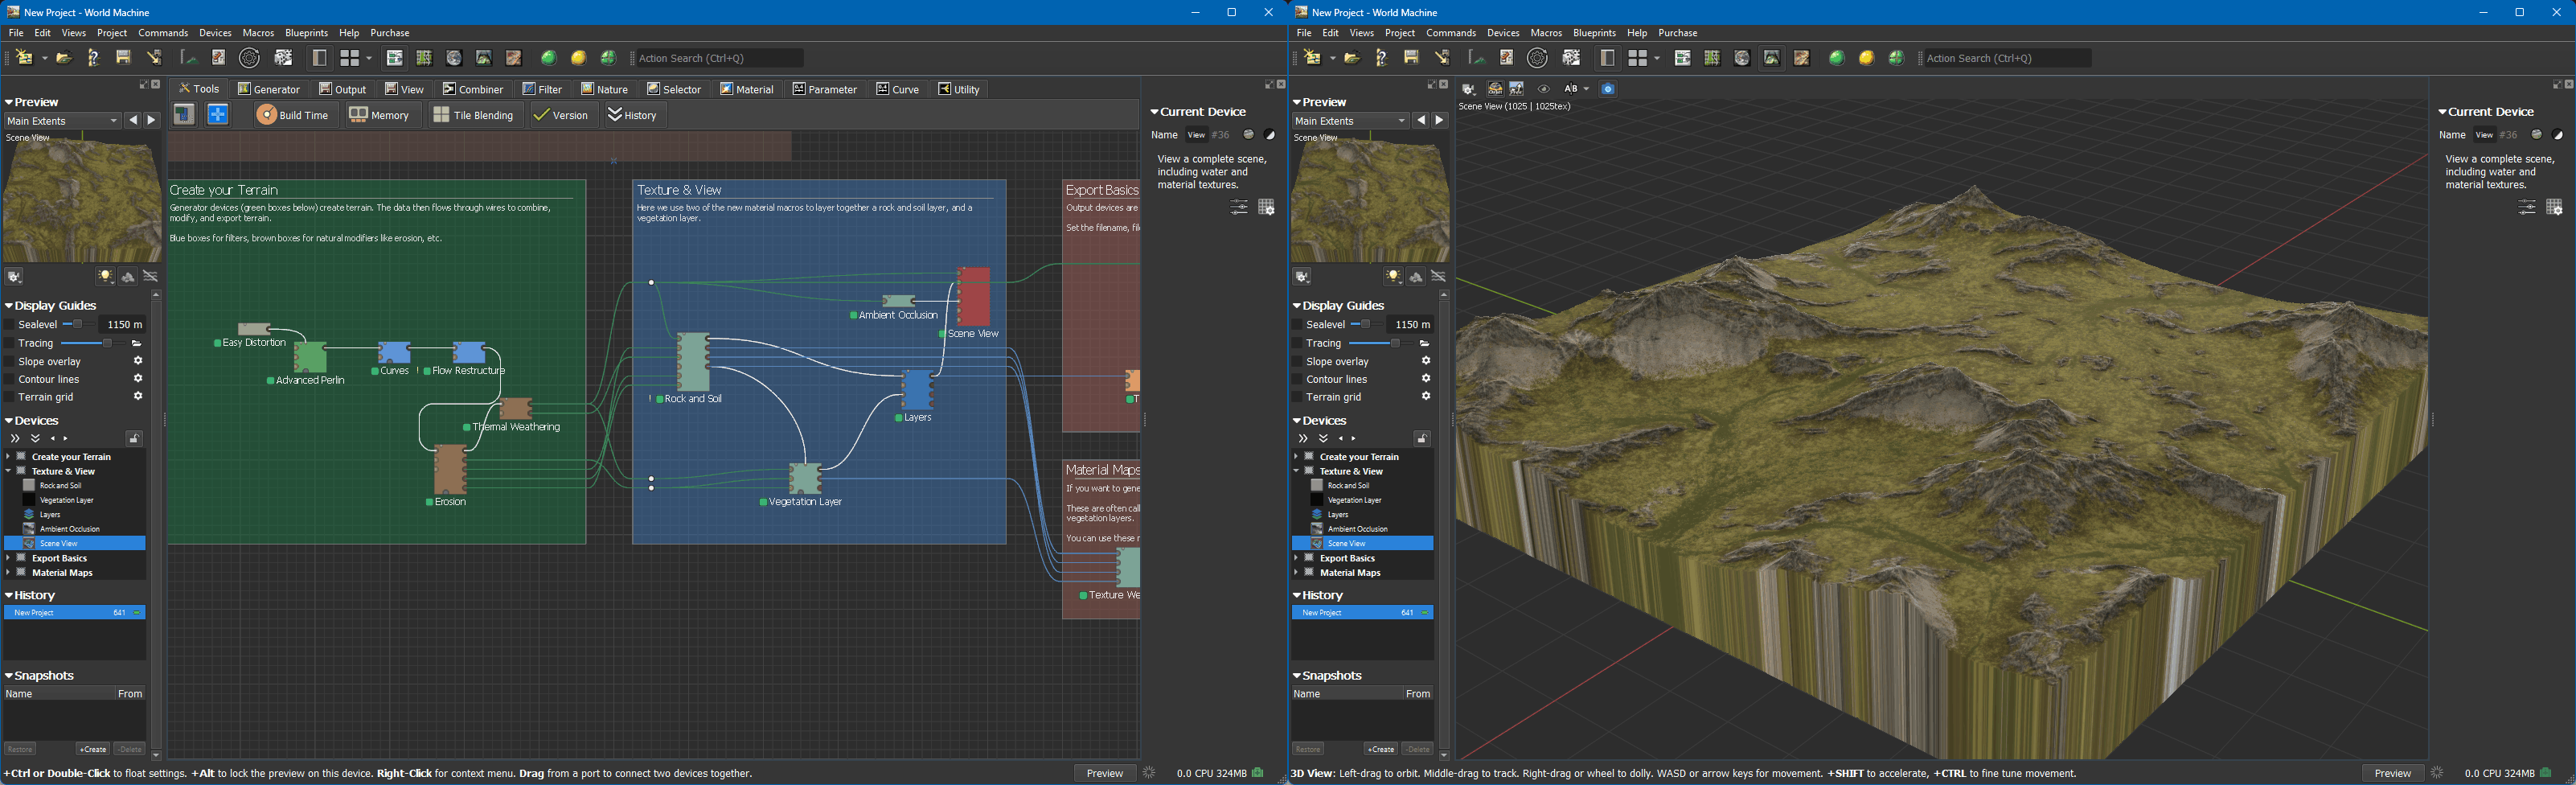
\includegraphics[width=1.0\textwidth]{obrazky-figures/world_machine_collage.png}
    \caption[World Machine Showcase]{World Machine terrain editor showcase. Node environment on the left. Render of the generated terrain on the right.}
    \label{fig:world_machine_showcase}
\end{figure}


\subsubsection{Blender}
Blender\footnote{Blender homepage: \href{https://www.blender.org/}{\texttt{www.blender.org}}}~\cite{blender_survey} is an open-source 3D editing, VFX, animation, rigging, sculpting, simulation, and rendering engine. It is a~versatile tool that covers practically every aspect of creating game assets, scenes, and more. It also features PCG tools in its pipeline, most notably the geometry node system and procedural materials. Blender also supports scripting and extensions, so users can freely use the capabilities of PCG, for example, with add-ons such as the A.N.T. Landscape\footnote{A.N.T. Landscape on Blender Extensions:~\href{https://extensions.blender.org/add-ons/antlandscape/}{\texttt{extensions.blender.org/add-ons/antlandscape}}}.

\subsubsection{Unreal Engine}
Unreal Engine\footnote{Unreal Engine homepage: \href{https://www.unrealengine.com/en-US}{\texttt{www.unrealengine.com/en-US}}}~\cite{game_dev_godot_and_other, unreal_engine_pcg} is a~state-of-the-art commercial multi-platform game, rendering, visualization, simulation, and animation engine developed by Epic Games and commonly used by game developers, as well as in the film and automotive industry. The projects are developed using a~component-based actor system. The engine uses graph-based blueprints and C++ for scripting and supports many features, including landscaping, visual shaders, animations, and advanced systems such as Lumen dynamic global illumination, Nanite virtualized micropolygon geometry, and a~full-featured PCG framework that allows creation and population of complex scenes based on defined rules and parameters. Support for voxel environments is available through third-party extensions such as the Voxel Plugin\footnote{Voxel Plugin for Unreal Engine homepage: \href{https://voxelplugin.com/}{\texttt{voxelplugin.com}}}.

\subsubsection{Unity}
Unity\footnote{Unity homepage: \href{https://unity.com/}{\texttt{unity.com}}}~\cite{game_dev_godot_and_other, unity_technical_survey} is a~widely used commercial multi-platform 2D and 3D game engine developed by Unity Technologies. Unity uses a~component-based game, level, and asset development system of game objects, similar to Unreal Engine. The engine uses C\# for scripting and offers a~feature-rich editor with support for animations, complex terrains, visual shaders, and many other features, including embedded SpeedTree support, with procedural vegetation generation capabilities. The engine is generally suitable for a~vast set of 2D and 3D projects. When it comes to PCG, Unity does not offer as many advanced features as the Unreal Engine PCG framework, but it can still be utilized. Voxels are not directly supported by the engine, but plugins such as Voxel~Play~3\footnote{Voxel Play 3:~\href{https://assetstore.unity.com/packages/tools/game-toolkits/voxel-play-3-310775}{\texttt{assetstore.unity.com/packages/tools/game-toolkits/voxel-play-3-310775}}} exist.

\begin{figure}[t]
    \centering
    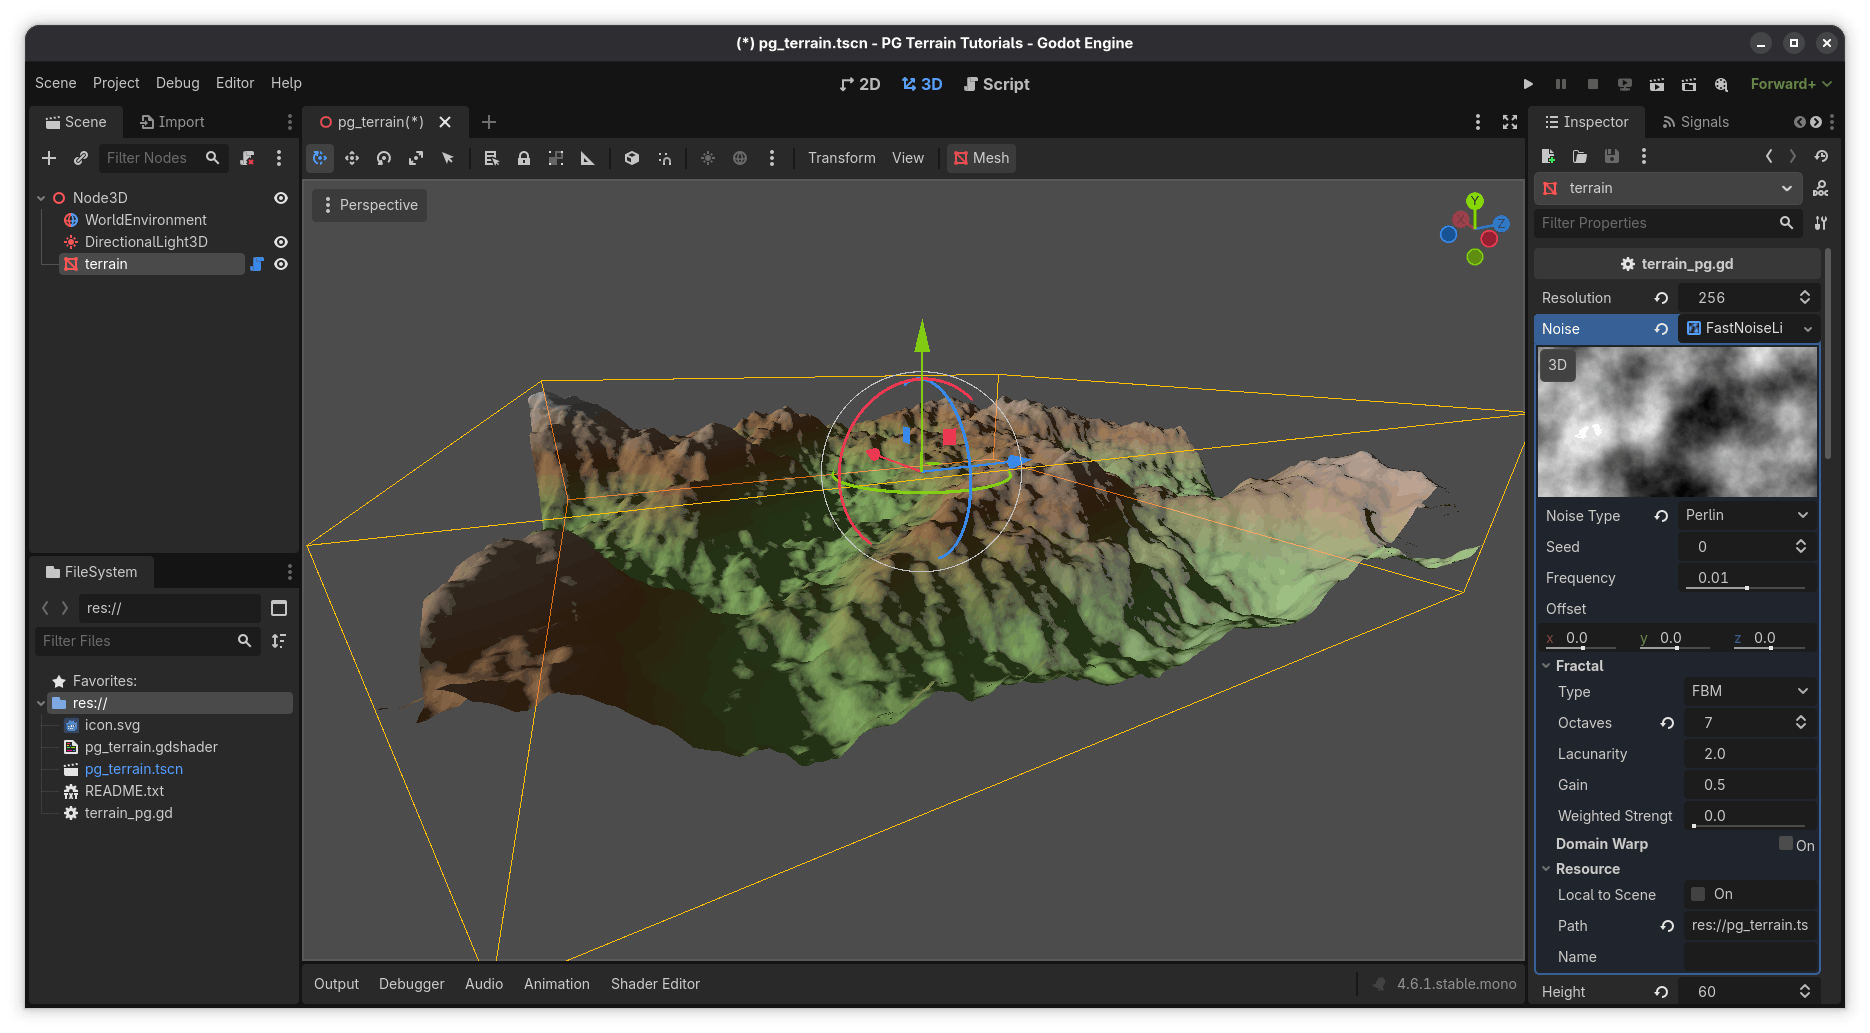
\includegraphics[width=0.6\textwidth]{obrazky-figures/godot_showcase.png}
    \caption[Godot Engine]{Procedural terrain showcase in the Godot Engine.}
    \label{fig:godot_showcase}
\end{figure}

\subsubsection{Godot Engine}
Godot Engine\footnote{Godot Engine homepage: \href{https://godotengine.org/}{\texttt{godotengine.org}}} is an open-source general-purpose 2D and 3D multi-platform game engine~\cite{game_dev_godot_and_other}. Games, their levels, and other components are created with a~versatile system of scenes and nodes. The engine features state-of-the-art support for 2D games and applications. Support for 3D is mature but not as advanced as in other engines, such as Unity or Unreal Engine. The engine is especially suitable for small and indie games. Larger, more complex projects might face difficulties due to the lack of features such as asset streaming. However, the engine can be easily extended. It supports scripting in multiple languages, including GDScript and C\#. However, it does not offer any built-in voxel features, and support for PCG is limited. Fortunately, third-party plugins and extensions exist, such as Voxel Tools for Godot\footnote{Voxel Tools for Godot on GitHub: \href{https://github.com/Zylann/godot_voxel}{\texttt{github.com/Zylann/godot\_voxel}}}. A showcase of the Godot Engine editor with procedurally generated terrain is in Fig.~\ref{fig:godot_showcase}.




\section{Showcase of Games Using PCG Techniques or Voxels}
In this section, a~selected set of games that use procedural content generation or voxel environments is showcased, and their use of these methods is briefly examined.

\subsection{Demoscene and .kkrieger}
Although the game .kkrieger~\cite{proc_gen_survey_mdpi} is just a~game demo, it should be mentioned due to its extensive use of PCG techniques. It was released in 2004 by a~demoscene group called Farbrausch, and it is a~third-person shooter game that fits within a~96~kB binary and, upon startup, uses PCG extensively to generate the game levels and all necessary assets, including textures, effects, animations, music, and more. A~showcase of the game is shown in Fig.~\ref{fig:games_collage}.

\begin{figure}[t]
    \centering
    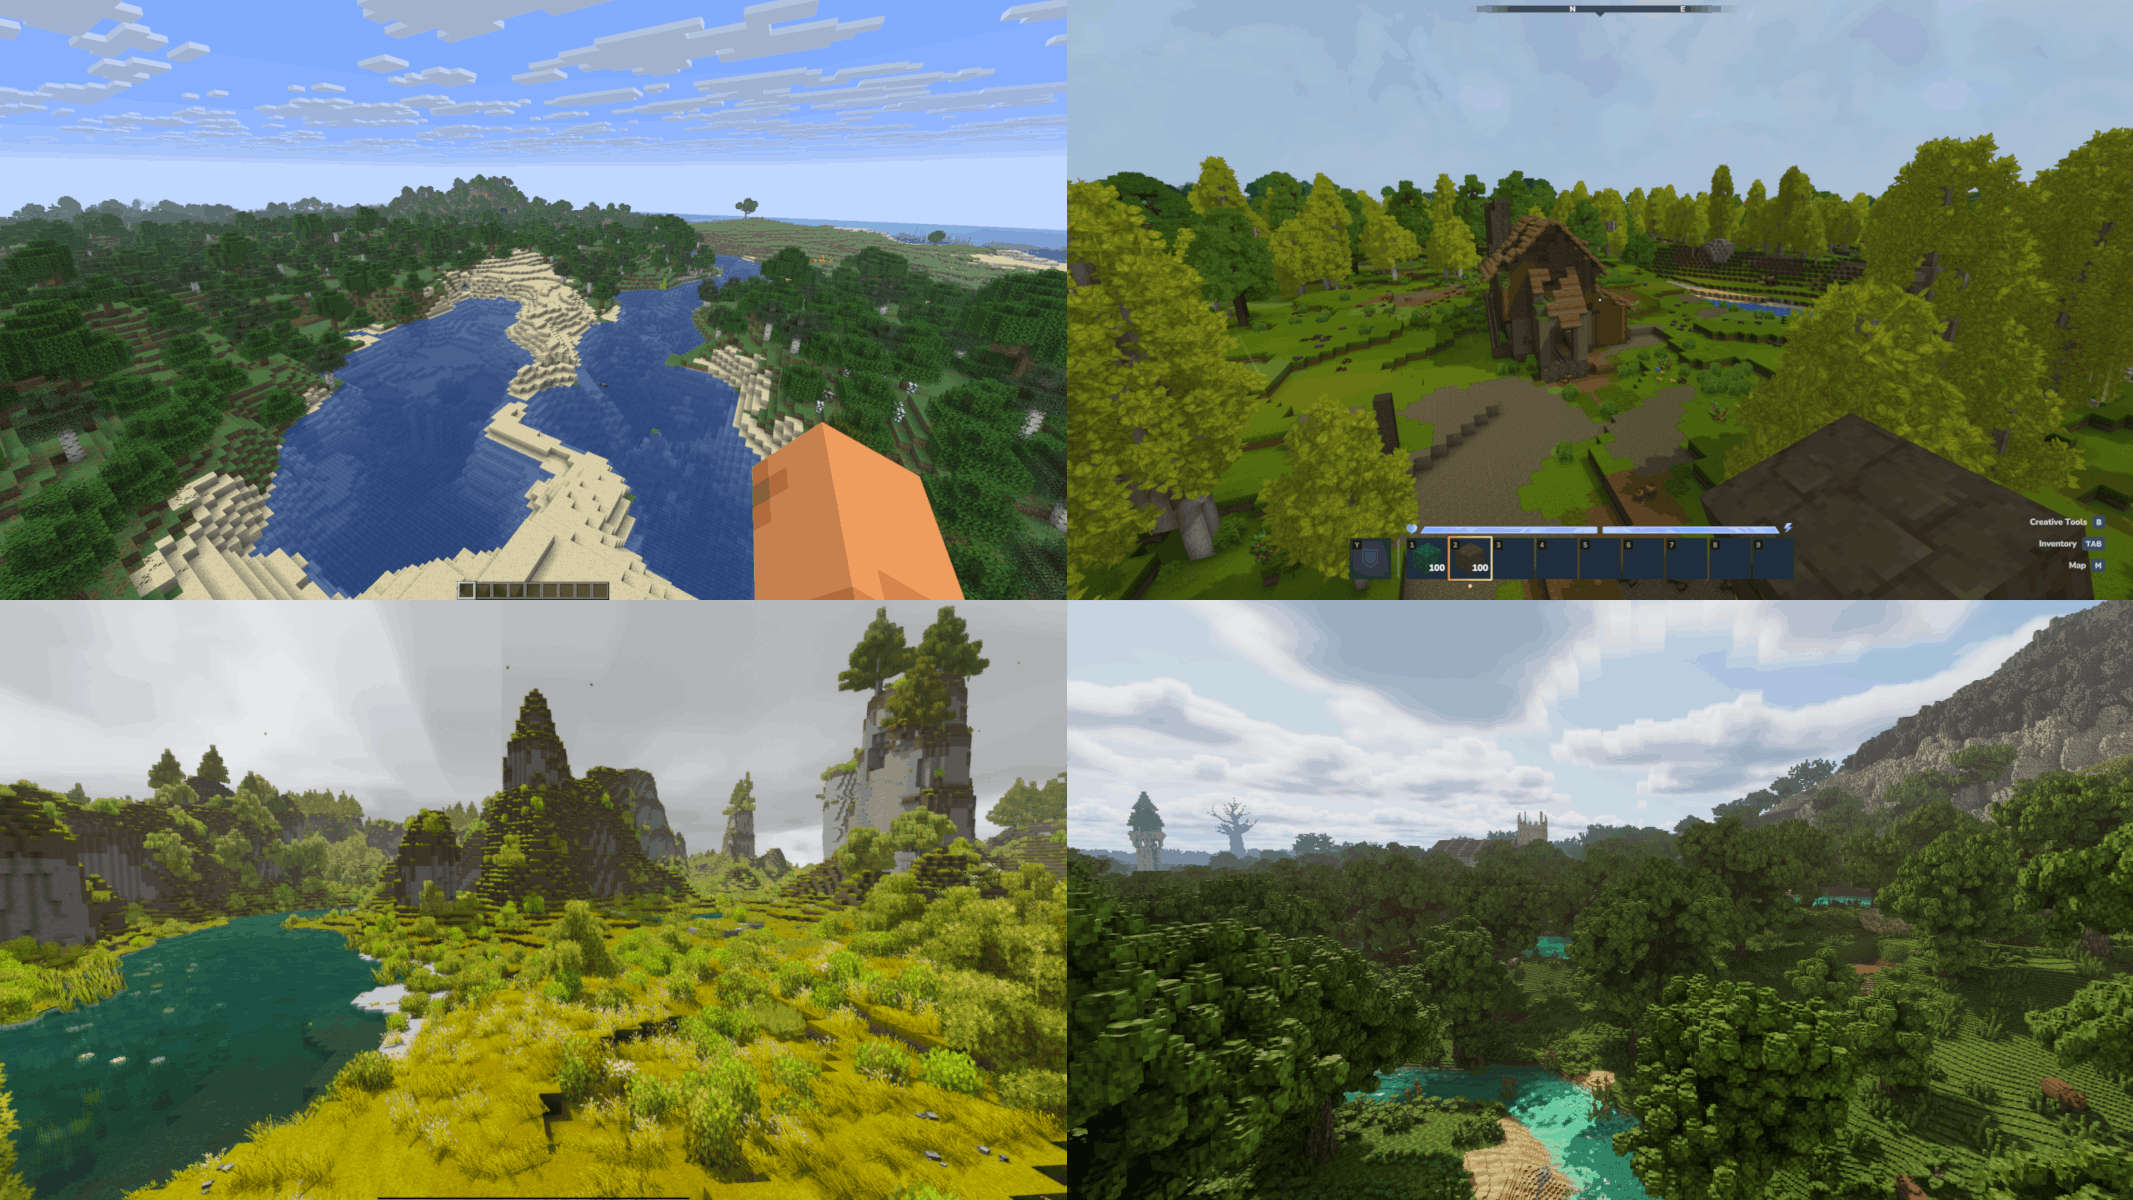
\includegraphics[width=1.0\textwidth]{obrazky-figures/sandbox_voxel_games_collage.png}
    \caption[Showcase of sandbox voxel games]{Showcase of selected sandbox voxel games. From left to right, top to bottom, Minecraft, Hytale, Vintage Story, and Lay of the Land.}
    \label{fig:sandbox_voxel_games_collage}
\end{figure}

\subsection{Sandbox Voxel Games}\label{sandbox-voxel-games}
With the release of Minecraft\footnote{Minecraft homepage: \href{https://www.minecraft.net/en-us/about-minecraft}{\texttt{www.minecraft.net/en-us/about-minecraft}}} in 2011, a~new type of game emerged, which could be called a~sandbox voxel game\footnote{The term ``sandbox voxel game'' is not official or widely used, but it was chosen in this thesis to relate to Minecraft-like voxel games with sandbox features and procedurally generated environments.}. Minecraft and its relatives, such as Vintage Story\footnote{Vintage Story homepage: \href{https://www.vintagestory.at/}{\texttt{www.vintagestory.at}}}, Hytale\footnote{Hytale homepage: \href{https://hytale.com/}{\texttt{hytale.com}}}, and Lay of the Land\footnote{Lay of the Land on Steam: \href{https://store.steampowered.com/app/2776090}{\texttt{store.steampowered.com/app/2776090}}}, feature vast procedurally generated voxel worlds composed of blocks. These worlds can be fully altered, allowing players to destroy and place blocks practically anywhere, unleashing their creativity. These games also usually feature survival mechanics and multiplayer, and their practically infinite, procedurally generated environments offer many opportunities for exploration. The environments of these games are shown in Fig.~\ref{fig:sandbox_voxel_games_collage}.



\subsection{Deep Rock Galactic}
Deep Rock Galactic\footnote{Deep Rock Galactic on Steam: \href{https://store.steampowered.com/app/548430}{\texttt{store.steampowered.com/app/548430}}} is a~co-op PvE FPS game, where players acting as dwarven space miners delve into deep caves to fight hordes of aliens and extract precious materials. The game features both PCG and voxel environments, with fully destructible, procedurally generated cavern systems. An example of a~cavern environment is shown in Fig.~\ref{fig:games_collage}.

\begin{figure}[t]
    \centering
    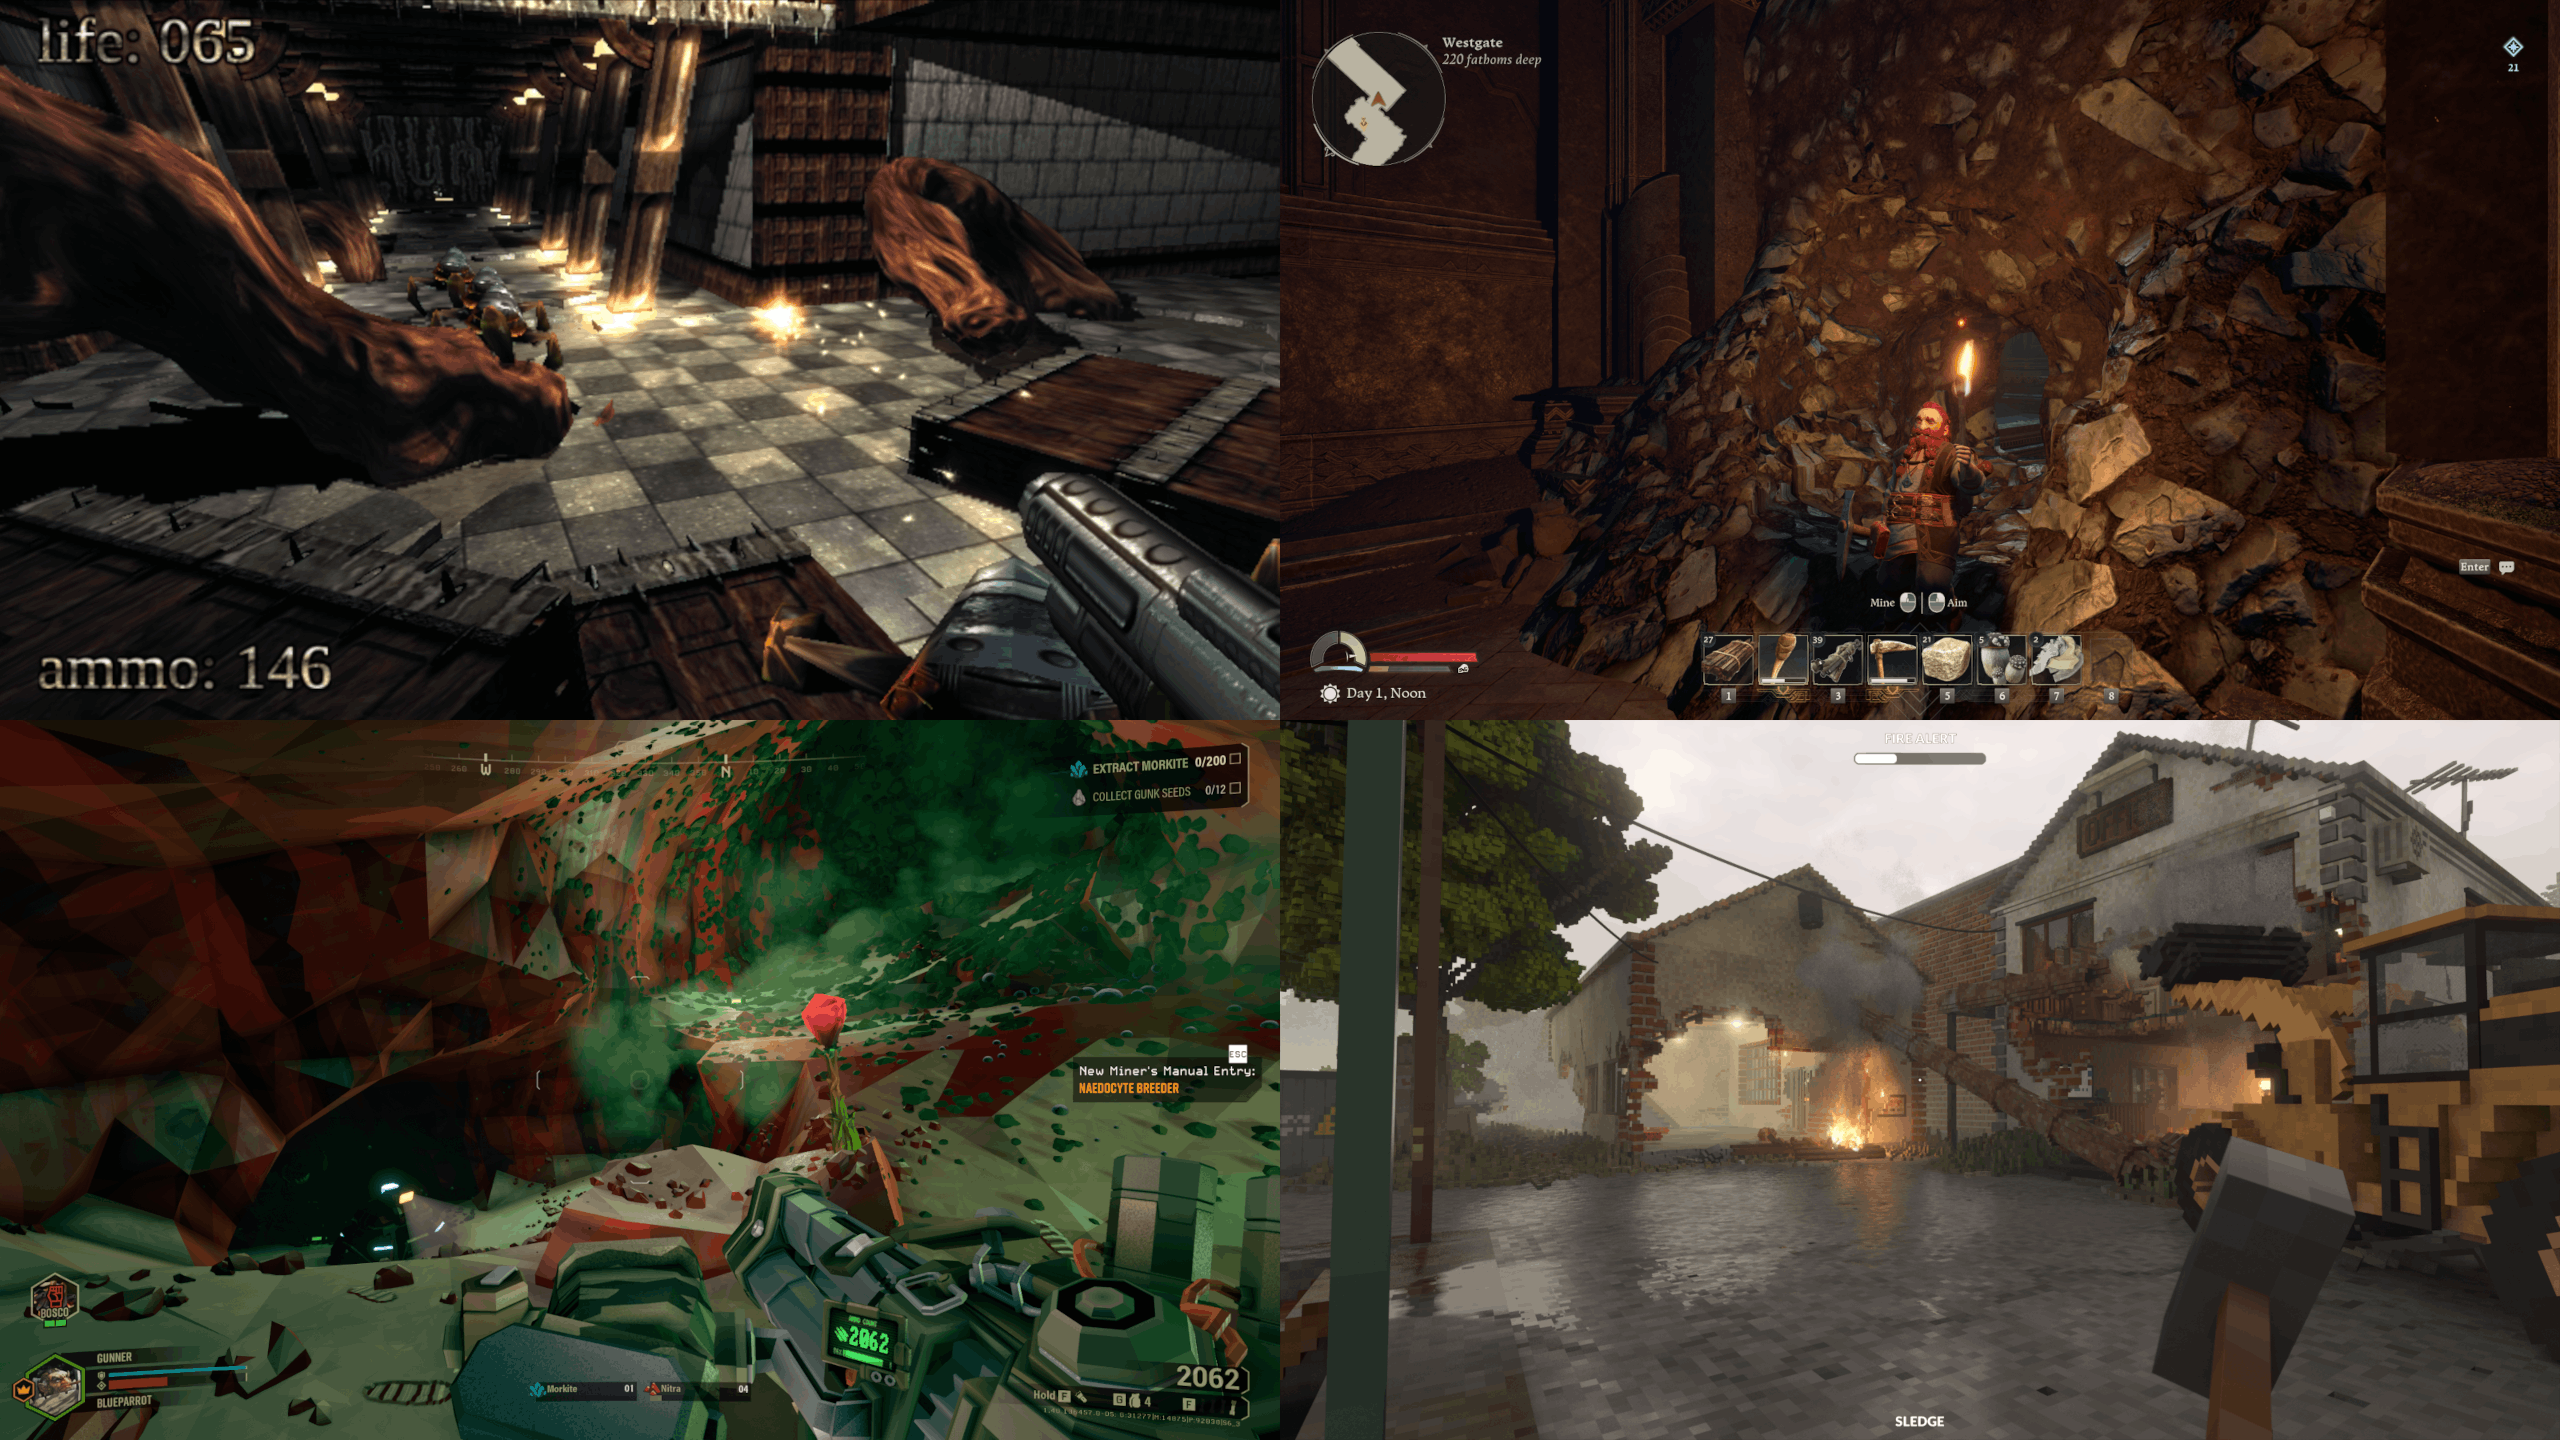
\includegraphics[width=1.0\textwidth]{obrazky-figures/games_collage.png}
    \caption[Games with Voxels and PCG]{Showcase of games that utilize PCG techniques or voxel environments. From left to right, top to bottom -- scene from .kkrieger demo, mineable areas in The Lord of the Rings: Return to Moria, and scenes from Deep Rock Galactic, and Teardown.}
    \label{fig:games_collage}
\end{figure}

\subsection{The Lord of the Rings: Return to Moria}
Return to Moria\footnote{The Lord of the Rings: Return to Moria on Steam: \href{https://store.steampowered.com/app/2933130}{\texttt{store.steampowered.com/app/2933130}}} is a~single-player and co-op survival crafting adventure set in the mines of Moria from the Lord of the Rings universe. Its environments are composed of procedurally generated level tiles and their contents. As a~result, the game's story, goals, and the overall structure of the cavern environment remain the same, whereas the locations of dungeons and details of the cavern environment change. The game also features many mineable voxel-based areas that can be interacted with to obtain specific resources, as shown in Fig.~\ref{fig:games_collage}.

\subsection{Teardown}
Teardown\footnote{Teardown on Steam: \href{https://store.steampowered.com/app/1167630/Teardown/}{\texttt{store.steampowered.com/app/1167630}}} is a~single-player and multiplayer destruction game, featuring fully destructible voxel worlds with a~high level of voxel detail, realistic physics, natural elements, and a~large set of drivable vehicles and tools. Example in-game footage can be seen in Fig.~\ref{fig:games_collage}. The game contains complex, high-definition voxel scenes, with per-voxel destruction and detailed physics and simulation of fire, water, and voxel debris.



%%%%%%%%%%%%%%%%%%%%%%%%%%%%%%
% Study of PCG Methods
%%%%%%%%%%%%%%%%%%%%%%%%%%%%%%
\chapter{Procedural Content Generation Methods}\label{proc-gen-methods}
This chapter provides an overview of procedural content generation methods that could be used for deterministic and stochastic creation of assets and environments in sandbox voxel game maps. The areas of study include pseudo-random number generators, procedural noise functions, various techniques based on formal theory, iterative methods, and sampling and depression-filling methods.

\section{Pseudo-Random Number Generation and Noise}
In this section, two of the most fundamental categories of procedural content generation methods are discussed, namely algorithms for pseudo-random number generation and procedural noises.

\subsection{Pseudo-Random Number Generation}
This section describes a~set of pseudo-random number generation (PRNG) methods suitable for procedural content generation. Generally, PRNGs can be used standalone for simple procedural content generation tasks. However, they primarily serve as the backbone for more advanced algorithms and methods that require random number generation.

\subsubsection*{Linear Congruential Generator}
A~linear congruential generator (LCG) is a~well-known method for producing a~sequence of pseudo-random, deterministic numbers~\cite{linear-congruential-generators-tezuka, peringer-hruby-ims, random-numbers-bikos}, often used in computer simulations. The generator is defined by recurrent Eq.~\ref{eq:lcg}, where $X_i$~is the previously generated number ($X_0$~is the initial value, often called a seed), $a$~is the multiplier, $c$~is the increment, and $m$~is the modulus. $X_{i+1}$ is the newly generated pseudo-random number. The ranges of the parameters are shown in Eq.~\ref{eq:lcg-ranges}.

\begin{equation}\label{eq:lcg}
    X_{i+1} = \left( a \cdot X_i + c \right)~\text{mod}~m
\end{equation}

\begin{equation}\label{eq:lcg-ranges}
\begin{aligned}
    0 < m \\
    0 < a < m \\
    0 \leq c < m
\end{aligned}
\end{equation}

The generation period depends on the parameters and is at most equal to $m$. To obtain a~value in the range $[0, 1)$, the resulting random number can be divided by the modulus, as can be seen in Eq.~\ref{eq:lcg-float}~\cite{linear-congruential-generators-tezuka}.  Generally, a~modulus that is a~power of two allows for an efficient LCG implementation.

\begin{equation}\label{eq:lcg-float}
    u_{i+1} = \frac{X_{i+1}}{m}
\end{equation}

The results of LCGs are highly dependent on the method parameters and are generated within an even distribution in the range $X_n \in \left[0, m\right)$~\cite{peringer-hruby-ims}. Most importantly, the following numbers in the sequence are not statistically independent of each other. The positives include a~very simple implementation and high performance.

\subsubsection*{Permuted Congruential Generator}
As with the LCG, the permuted congruential generator~\cite{oneill:pcg2014} is a~method for generating deterministic pseudo-random numbers. Its main goal is to improve the statistical properties of power-of-two LCGs while still offering their high performance.

It works by applying permutations to the output of a~power-of-two LCG. There are several variants of output permutations in the family of these generators, each with different properties. The recommended variation \emph{PCG-XSH-RR}~\cite{oneill:pcg2014} uses a~$64$-bit state, has a~$32$-bit output, and its transformation function can be seen in List.~\ref{code:pcg-xsh-rr}, where \texttt{rot32(v, r)} denotes a~clockwise bit rotation of \emph{r} bits on \emph{v}.

\begin{lstlisting}[caption={Transformation function for PCG-XSH-RR.}, label={code:pcg-xsh-rr}]
        output = rot32((state ^ (state >> 18)) >> 27, state >> 59)
\end{lstlisting}

As described in the report~\cite{oneill:pcg2014}, this variation uses \emph{xorshift} to improve the high bits and then randomly rotates them, so that all bits become full period. In this case, the top 5~bits are used to specify the rotation, and thus the constants are 18 for \emph{xorshift} mixing (half of the necessary 37 bits (32 output, 5~rotation)), 27 to obtain the $32$-bit output (5~bits already used for rotation ($64 - 32 - 5 = 27$) and then 59 to obtain the top 5 bits for rotation.

The permuted congruential generator is a~fast, statistically correct method for generating pseudo-random numbers. Its high speed enables its application in various areas of computer technology, including the procedural and runtime generation of content. Due to its good statistical properties, it should not cause any problems with repeating patterns.


\subsubsection*{Xorshift}
Xorshift~\cite{marsaglia-xorshift} is another method for pseudo-random number generation. The very simple implementation that uses just a~few \emph{xorshift} operations (exclusive \emph{or} (\emph{xor}) applied to an n-bit word with a~shifted version of itself), is rather fast and produces usable random numbers.

The method relies on the already described \emph{xorshift} operation. Both versions (right and left shifts) are shown in List.~\ref{code:xorshift-basic}. It can be seen that the $n$-bit word \emph{y}~is first shifted right or left by \emph{m}~bits, and then the \emph{xor}~operation is applied to it and its original version. This effectively mixes the bits together and, with repeated application, leads to randomization.

\begin{lstlisting}[caption={Xorshift operation.}, label={code:xorshift-basic}]
                            result = (y ^ (y >> m))
                            result = (y ^ (y << m))
\end{lstlisting}

Of course, there are many possible applications of \emph{xorshifts} for random number generation. Their primary difference is the number of \emph{xorshift} operations, and the values of the constants used for the bit shifts\footnote{Example implementations and comparisons can be seen in the original paper by Marsaglia~\cite{marsaglia-xorshift}.}. One $32$-bit variation~\cite{marsaglia-xorshift} is shown in List.~\ref{code:xorshift-example-code}.

\begin{lstlisting}[caption={32-bit example xorshift implementation.}, label={code:xorshift-example-code}]
    unsigned long xor() {
        static unsigned long y = 2463534242;
        y ^= (y << 13);
        y ^= (y >> 17);
        return (y ^= (y << 5));
    }
\end{lstlisting}

The resulting random numbers of the \emph{xorshift} method are of good quality~\cite{marsaglia-xorshift} and usable in various fields of computer technology. However, there are better modern methods that have similar performance but significantly better statistical properties\footnote{Comparisons can be seen in report~\cite{oneill:pcg2014}.}, such as the already described PCG method.

\subsubsection*{Summary of Pseudo-Random Number Generators}
Pseudo-random number generators are the oldest and simplest of methods used for procedural content generation in games~\cite{proc-cont-gen-games-survey-hendrikx}. Their ability to introduce randomness into game content still plays a~significant role in procedural content generation today, and these methods are used in both simple content generators and as a~backbone for more advanced, modern methods.

\subsection{Procedural Noise Functions}\label{proc_noise_functions}
This section describes another classical tool used in procedural content generation -- procedural noise functions. Whereas PRNGs produce random, unrelated values, procedural noise functions are continuous and smooth, making them suitable for creating natural patterns. The parameters and advantages of procedural noise as described in a survey~\cite{lagae-proc-noise-survey} are the following:

\begin{itemize}
    \item Procedural noise is continuous, smooth, multi-resolution, and it does not depend on discretely sampled data.
    \item It is non-periodic and thus capable of filling any-dimensional space.
    \item It is configurable and can be accessed randomly, allowing parallelization.
    \item Most noise functions are also compact in space, both memory and code-wise.
\end{itemize}

The following sections describe value noise, Perlin and Simplex noises, cellular Worley noise, and fractal Brownian motion. These appear to be industry standards with numerous applications.


\subsubsection*{Value Noise}
Value noise\footnote{Scratchapixel blog post:~\href{https://www.scratchapixel.com/lessons/procedural-generation-virtual-worlds/procedural-patterns-noise-part-1/introduction.html}{\texttt{www.scratchapixel.com/lessons/procedural-generation-virtual-worlds /procedural-patterns-noise-part-1/introduction.html}} }~\cite{procedural-terrain-archer, scratchapixel} is a~very simple noise implementation with minimal performance cost. For its 2D version, a~regular 2D grid can be used, with randomly generated points. The output of the noise function is then the interpolated value based on the surrounding grid points for the given input coordinates. A~detailed description~\cite{procedural-terrain-archer, scratchapixel} follows:

\begin{enumerate}
    \item Firstly, it is necessary to remap the coordinates of the input position to the noise grid and obtain its closest grid points together with distances to them.
    \item Then, random values for the grid points are calculated or obtained from a~predefined set, usually via a~permutation table.
    \item Before interpolating the values at grid points, the distances to the grid points should be smoothed out by remapping. One possible remapping function is $3t^2 - 2t^3$.
    \item These values are then interpolated based on the remapped distances of their relative grid points to the input point.
    \item The resulting interpolated scalar is the value of the noise at the given position.
\end{enumerate}

\begin{figure}[t]
    \centering
    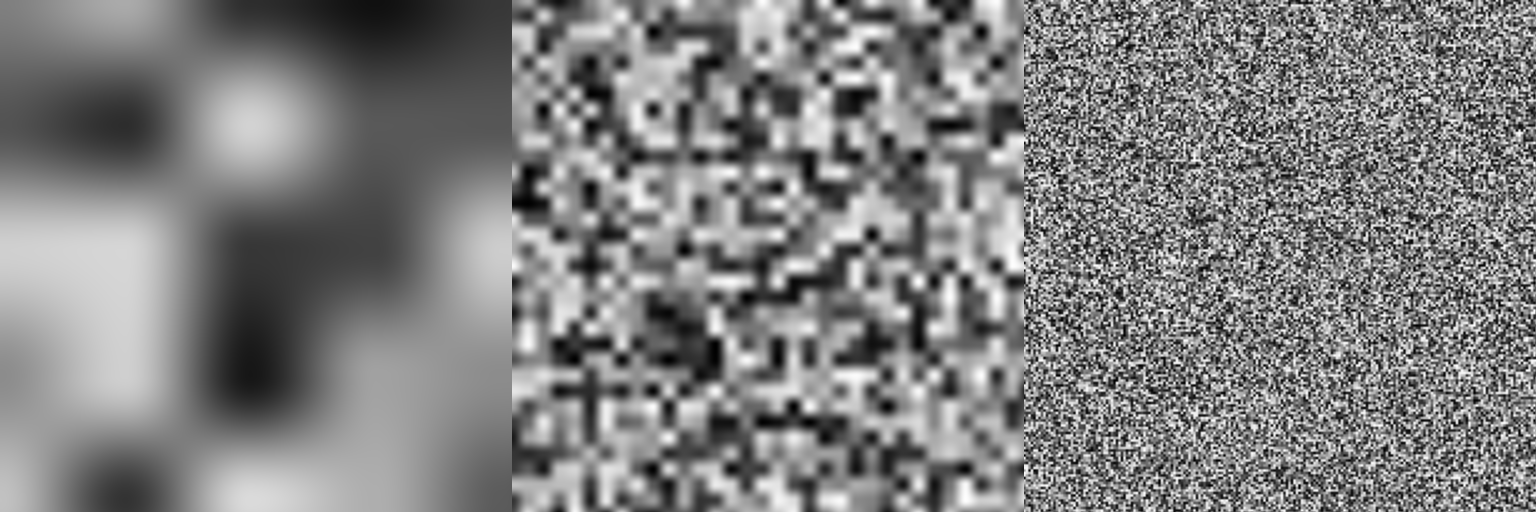
\includegraphics[width=0.6\textwidth]{obrazky-figures/noise/valueCombined.png}
    \caption{Visualization of 2D value noise with increasing frequency (left to right).}
    \label{fig:noise-value-basic}
\end{figure}

Value noise (see Fig.~\ref{fig:noise-value-basic}) is a~simple and fast noise function that can be used in procedural content generation. However, its low quality severely limits its potential applications, especially when better noise functions, such as Perlin or Simplex, are available.

\subsubsection*{Perlin Noise}
Perlin noise\footnote{Perlin's online presentation:~\href{https://web.archive.org/web/20071011035810/http://noisemachine.com/talk1/}{\texttt{web.archive.org/web/20071011035810/http://noisemachine.com/talk1}}}~\cite{perlin-image-synthesizer} is a~very important procedural noise function. The algorithm itself is very similar to the value noise described above in terms of its use of grid structures and interpolation. However, there is one main difference: it is a~gradient noise. The use of gradients and other enhancements enables it to have significantly better properties than value noise.

The algorithm\footnote{Scratchapixel blog post:~\href{https://www.scratchapixel.com/lessons/procedural-generation-virtual-worlds/perlin-noise-part-2/perlin-noise.html}{\texttt{www.scratchapixel.com/lessons/procedural-generation-virtual-worlds /perlin-noise-part-2/perlin-noise.html}}}~\cite{gustavson-simplex-noise, perlin-image-synthesizer, scratchapixel} uses an $n$-dimensional grid, where each grid point (cell corner) has a~fixed pseudo-random $n$-dimensional gradient vector of unit-length associated with it. This can be seen in Fig.~\ref{fig:perlin-grid-gradient}. 



When calculating the noise value for a~given set of coordinates, these coordinates must be remapped to the grid structure (similar to value noise) to determine the grid cell in which the evaluated point lies. Then, it is necessary to find the $2^n$ cell corners, along with the values of their gradient vectors. Again, these can be obtained similarly to value noise, using a~permutation table that selects from a~predefined set of gradient vectors. After that, the offset vectors can be calculated from the cell corners to the evaluation point. Then, the dot product between each cell corner's gradient vector and the offset vector to the evaluation point is calculated. Finally, the resulting $2^n$ dot products are interpolated to obtain the noise value at a~given set of coordinates. This interpolation is performed with a~function that has zero first derivative at the $2^n$ grid points, possibly $3t^2 - 2t^3$~\cite{perlin-improving-noise, gustavson-simplex-noise, perlin-image-synthesizer}.

\begin{figure}[t]
    \centering
    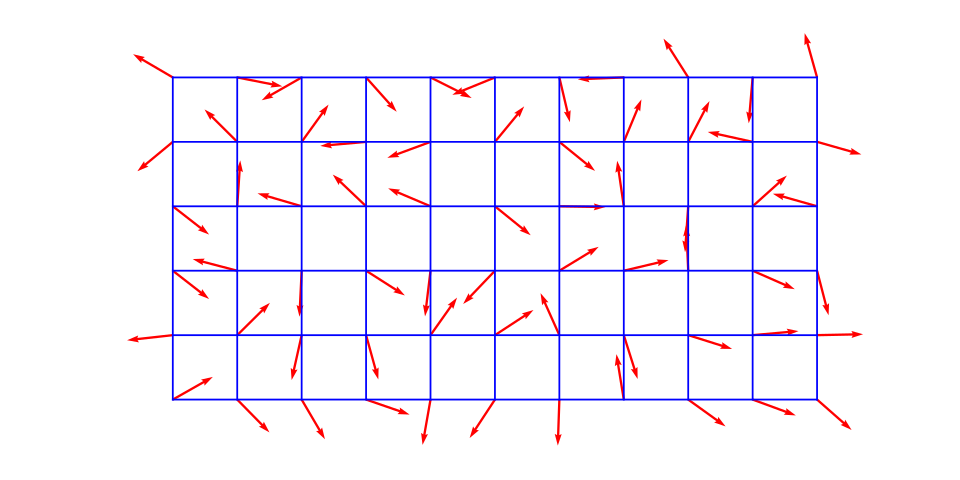
\includegraphics[width=0.5\textwidth]{obrazky-figures/noise/perlin-gradient-wiki.png}
    \caption[Perlin noise gradient grid]{2D grid with gradient vectors for generation of Perlin noise.\footnotemark}
    \label{fig:perlin-grid-gradient}
\end{figure}

\footnotetext{Image source: \href{https://en.wikipedia.org/wiki/File:PerlinNoiseGradientGrid.svg}{\texttt{en.wikipedia.org/wiki/File:PerlinNoiseGradientGrid.svg}}}

\begin{figure}[b]
    \centering
    
\includegraphics[width=0.6\textwidth]{obrazky-figures/noise/perlinCombined.png}
    \caption[Perlin noise visualization]{Visualization of 2D Perlin noise with increasing frequency (left to right).}
    \label{fig:noise-perlin-basic}
\end{figure}

Perlin noise (see Fig.~\ref{fig:noise-perlin-basic}) is a~very important procedural noise function with better properties than the discussed value noise. However, it has its issues, including the complexity $O\left(2^n\right)$, which becomes cumbersome in higher dimensions, problems with visible grid patterns~\cite{perlin-improving-noise}, and more.

\subsubsection*{Simplex Noise}
Simplex noise~\cite{gustavson-simplex-noise} is another procedural noise function, developed to overcome the issues of Perlin noise. As shown in Fig.~\ref{fig:noise-simplex-basic}, it is visually distinct. Its advantages over Perlin noise include lower computational complexity, better scaling in higher dimensions (complexity is $O\left(n^2\right)$), and no noticeable directional artifacts. The results of the function also better conform to the original noise specifications described in~\cite{perlin-image-synthesizer}.

Its main difference lies in using simplices rather than hypercubes for its grid structure. This change radically reduces the number of corners that need to be visited during noise calculation from $2^n$ to $n$ for the $n$-th dimension. Another important difference is the use of the summation of contributions from corners rather than their interpolation. These contributions are multiplications of the extrapolation of the gradient ramp and a~radially symmetric attenuation function (as described in~\cite{gustavson-simplex-noise}). Radial attenuation is chosen so that the computation of noise for points in each simplex is not influenced by its neighbors. Thus, only the corners of that particular simplex influence the computation of noise inside it, which decreases the overall computational cost~\cite{gustavson-simplex-noise}.

\begin{figure}[t]
    \centering
    
\includegraphics[width=0.6\textwidth]{obrazky-figures/noise/simplexCombined.png}
    \caption[Simplex noise visualization]{Visualization of 2D Simplex noise with increasing frequency (left to right).\footnotemark}
    \label{fig:noise-simplex-basic}
\end{figure}

\footnotetext{Simplex noise implementation described by Stephan Gustavson in article~\cite{gustavson-simplex-noise} was utilized.}

\subsubsection*{Worley Noise}
Worley noise~\cite{worley-noise} is another procedural noise function. It is especially helpful in creating natural cellular patterns (see Fig.~\ref{fig:noise-worley-basic}). It was designed in 1996 by Steven Worley~\cite{worley-noise} to complement other procedural noise functions.

It works by specifying a~grid of feature points and then calculating the distances to the $n$ closest feature points from a~requested location. For this, a~basis function $F_n\left(x\right)$ is used that calculates the distance to the $n$-th closest feature point from location $x$. The values of $F_1\left(x\right), F_2\left(x\right), ..., F_n\left(x\right)$ are then the results of the noise for a~given position $x$ and the set of closest points.

\begin{figure}[b]
    \centering
    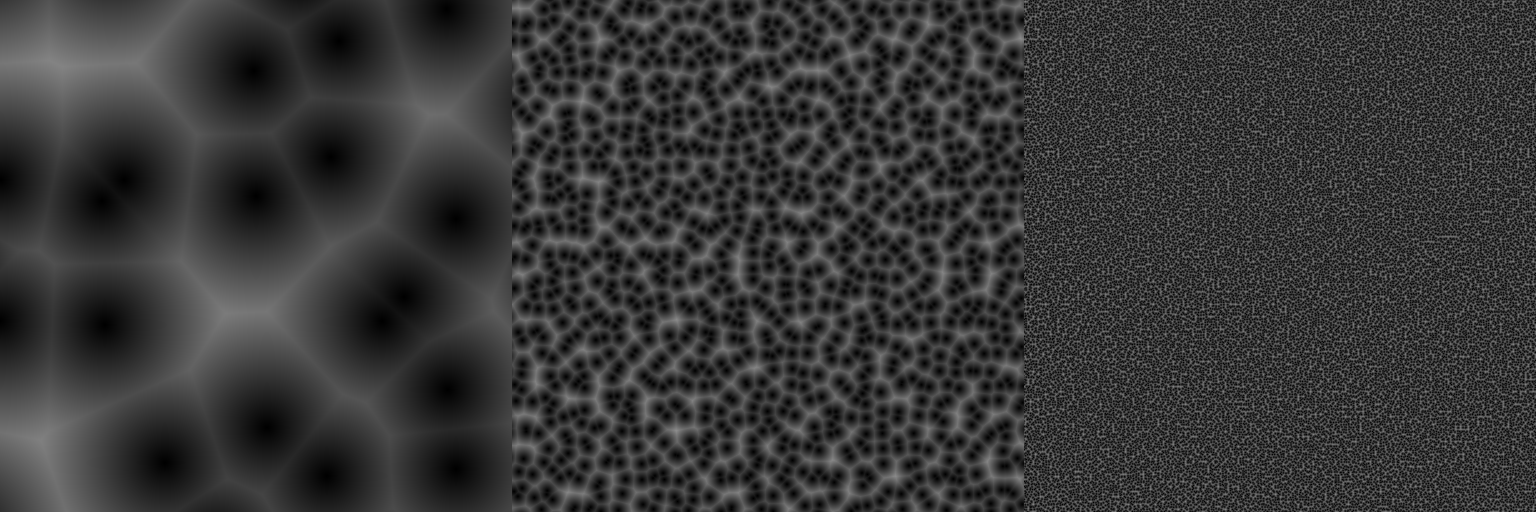
\includegraphics[width=0.6\textwidth]{obrazky-figures/noise/cellularCombined.png}
    \caption[Worley noise visualization]{Visualization of 2D Worley noise with increasing frequency (left to right).}
    \label{fig:noise-worley-basic}
\end{figure}

The first step in the evaluation of the function $F_n\left(x\right)$ is the generation of feature points. For this, a~Poisson distribution is used to ensure that the points are uniformly distributed. In the 3D version of Worley noise, space is divided into a~grid of cubes, and the points are generated in them. The actual number of points in each cube is specified by a~predefined probability table generated from a~Poisson distribution. To select a~specific number of points and then determine their positions, random numbers are generated using an LCG with its seed initialized to a~hash of the integer coordinates of the current grid cube. This way, the input position is translated to a~cube on the grid, and its feature points are generated, along with the calculations of their distances to the input position. At the end of this step, a~sorted list of the closest distances inside the cube is obtained. However, there might be closer feature points in the neighboring cubes. So, these cubes must be iterated over as well. Fortunately, this can be optimized, and many neighboring cubes can be skipped based on the closest feature points that were already found~\cite{worley-noise}.


\subsubsection*{Fractal Brownian Motion Noise}\label{fbm_noise}
Instead of using the noises described above directly, multiple noise layers can be combined, each with varying parameters, to create more natural-looking patterns. This is often described as fractal Brownian motion (fBm) noise\footnote{Scratchapixel blog post:~\href{https://www.scratchapixel.com/lessons/procedural-generation-virtual-worlds/procedural-patterns-noise-part-1/simple-pattern-examples.html}{\texttt{www.scratchapixel.com/lessons/procedural-generation-virtual- worlds/procedural-patterns-noise-part-1/simple-pattern-examples.html}}}~\cite{perlin-image-synthesizer, scratchapixel, thebookofshaders}, or octave noise. In each octave, the noise layer's frequency is typically doubled, and its amplitude is halved. With this approach, self-similarity is introduced in features of all sizes. This is a~typical characteristic of natural patterns, as terrain does not only consist of large hills and deep valleys (low frequency, high amplitude), but rather has these features repeated at smaller levels of detail, such as small hills, ravines, and rocky areas (up to high frequency, low amplitude). Visual comparison of non-fBm and fBm terrain is shown in Fig.~\ref{fig:noise-fractal-terrain}.

Mathematically, the computation of $n$~octave noise would be written as a~sum of multiple layers of noise. This can be seen in Eq.~\ref{eq:fbm} where $f_0$~is the base frequency, $L$~stands for lacunarity (scaling of frequency, typically $2$), $g$~stands for gain (scaling of amplitude, usually $0.5$), and $x$~is the position vector of the requested noise value.

\begin{equation}\label{eq:fbm}
    \mathit{fBm}(x) = \sum_{k = 0}^{n-1} noise\left(x\, f_0\, L^k \right) g^k
\end{equation}


\begin{figure}[b]
    \centering
    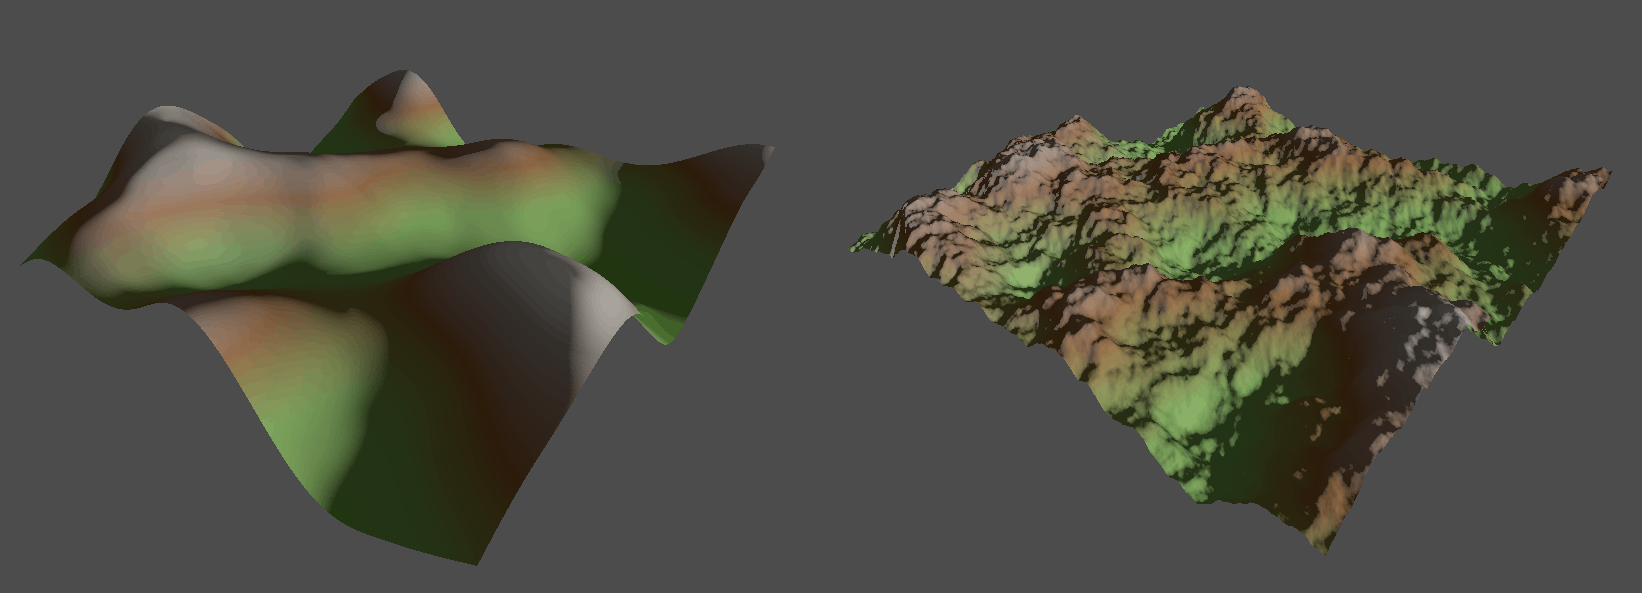
\includegraphics[width=0.6\textwidth]{obrazky-figures/noise/fractal_terrain.png}
    \caption[Perlin noise terrain visualization]{Visualization of a~shaded terrain created with 2D Perlin noise values as a~height map. Basic Perlin noise on the left and Perlin noise with fBm on the right.}
    \label{fig:noise-fractal-terrain}
\end{figure}

\subsubsection*{Summary of Procedural Noise Functions}

Procedural noise functions, and their possible transformations, are among the most important PCG methods. They can be used to generate animations, gradients, natural-looking textures, terrain height maps, and volumetric properties of 3D shapes~\cite{lagae-proc-noise-survey, proc_gen_survey_mdpi}.


\section{Iterative Methods, Grammars, and Automata}
In this section, a~set of iterative methods is presented, mostly based on formal grammars and automata theory, that are usable for procedural content generation. Namely, L-systems and cellular automata are discussed. This section also contains the iterative Space Colonization algorithm, which can be used to generate realistic-looking trees and bushes.

\subsection{L-systems}
L-systems~\cite{l-systems-lindenmayer-1968, developmental-systems-l-systems} or Lindenmayer systems, proposed in the 1960s by Aristid Lindenmayer and his colleagues~\cite{l-systems-lindenmayer-1968, developmental-systems-l-systems} for the description of the growth of plants and other living organisms, are parallel rewriting systems. They are usually defined as a~triplet (Eq.~\ref{eq:l-systems}), where $V$~is a~set of terminal and nonterminal symbols, $\omega$~denotes the initializing string that contains the starting set of terminals and nonterminals, and $P$~stands for a~set of production rules that are applied to the current string of symbols and transform these into other sets of terminals and nonterminals in parallel. A~possible example of a~production rule can be $A \rightarrow Ab$, which transforms a~nonterminal $A$~into a~string with a~nonterminal $A$~and a~terminal $b$.

\begin{equation}\label{eq:l-systems}
    G = \left(V, \omega, P\right)
\end{equation}

There are various types of L-systems that allow for differing constructions and capabilities~\cite{developmental-systems-l-systems, l-systems-lindenmayer-1968, l-systems-application-1, l-systems-application-2}. The most basic form of L-systems is D0L-systems, which define deterministic context-free L-systems. Another example is the Stochastic L-system, which allows multiple production rules with the same left-hand side. These rules are then assigned a~probability, and thus the derivation of these L-systems allows for randomization of their outputs.

For the visualization of structures generated by L-systems, turtle graphics and other techniques were often used~\cite{l-systems-application-1, l-systems-application-2}, with the necessary control commands written directly as terminals of the generated strings.
 
L-systems are used primarily for the procedural generation of vegetation~\cite{proc-cont-gen-games-survey-hendrikx, l-systems-application-1, l-systems-application-2}, particularly trees and plants. However, the strong formal basis enables them to generate many patterns, or even entire rooms or game levels.

\subsection{Cellular Automata}
Cellular automata~\cite{peringer-hruby-ims, cellular-automata-theory-kari} are typically discrete models of computation. They consist of a~grid of cells, where each cell represents a~basic element that can be in one of the defined states. The state of a~selected cell at a~given time depends on the states of its neighbors within its defined neighborhood and the cell's own state at the previous time step. The function defining these state transitions can be seen in Eq.~\ref{eq:ca-f-def}, where $t$~is the current time, the function $s\left(time\right)$ defines the state of a~cell at a~given time, and $N_s\left(time\right)$ defines the effect from its neighborhood at a~given time.

\begin{equation}\label{eq:ca-f-def}
    s\left(t  + 1\right) = f\left(s\left(t\right), N_s\left(t\right)\right)
\end{equation}

Typical applications of cellular automata are in various simulations. When it comes to procedural content generation, they can be used to generate textures and patterns, or their simulation results can be used to specify feature placement~\cite{proc-cont-gen-games-survey-hendrikx}.

\subsection{Space Colonization Algorithm}\label{space-col-algo}
The Space Colonization algorithm~\cite{space-colonization} is a~3D extension of the open leaf venation model~\cite{leaf-venation}, with the primary goal of creating 3D branching structures. Its key idea is the iterative addition of nodes to a~tree structure based on competition for space.

The algorithm starts with a~defined set of attraction points and a~single starting node. The attraction points represent the available space into which the tree structure will iteratively grow from the starting node. In each iteration, an attraction point may influence its closest tree node. This happens when their distance is smaller than a~defined radius of influence~$d_i$. Several attraction points can influence a~single node in an iteration, denoted by a~set of points $S\left(v\right)$. In the case where $S\left(v\right)$ is not empty, a~new node $v'$ is created and attached to its parent node $v$ by a~new segment $\left(v, v'\right)$. This new node is positioned at a~distance $D$~from the parent node $v$~in the direction of the average of normalized vectors toward all attraction points $s \in S\left(v\right)$ that influenced the creation of this node. Thus, $v'$~is computed by $v' = v  + D\hat{n}$, where $\hat{n}$~is the average of normalized vectors (Eq.~\ref{eq:space-col-normalized}). The direction of growth can be optionally biased with the use of a~bias vector $\vec{g}$~that represents effects such as branch weight and tropisms. Its application is shown in Eq.~\ref{eq:space-col-bias}. After the addition of new nodes, the iteration continues with the removal of all attraction points that are closer to any node than a~kill distance threshold $d_k$~\cite{space-colonization}.

\begin{equation}
    \hat{n} = \frac{\vec{n}}{\lVert \vec{n} \rVert} \quad \text{and} \quad  \vec{n} = \sum_{s \in  S\left( v \right)} \frac{s - v}{\lVert s - v \lVert}
    \label{eq:space-col-normalized}
\end{equation}

\begin{equation}
    \hat{n} = \frac{\hat{n} + \vec{g}}{\lVert \hat{n} + \vec{g} \rVert}
    \label{eq:space-col-bias}
\end{equation}

\begin{figure}[t]
    \centering
    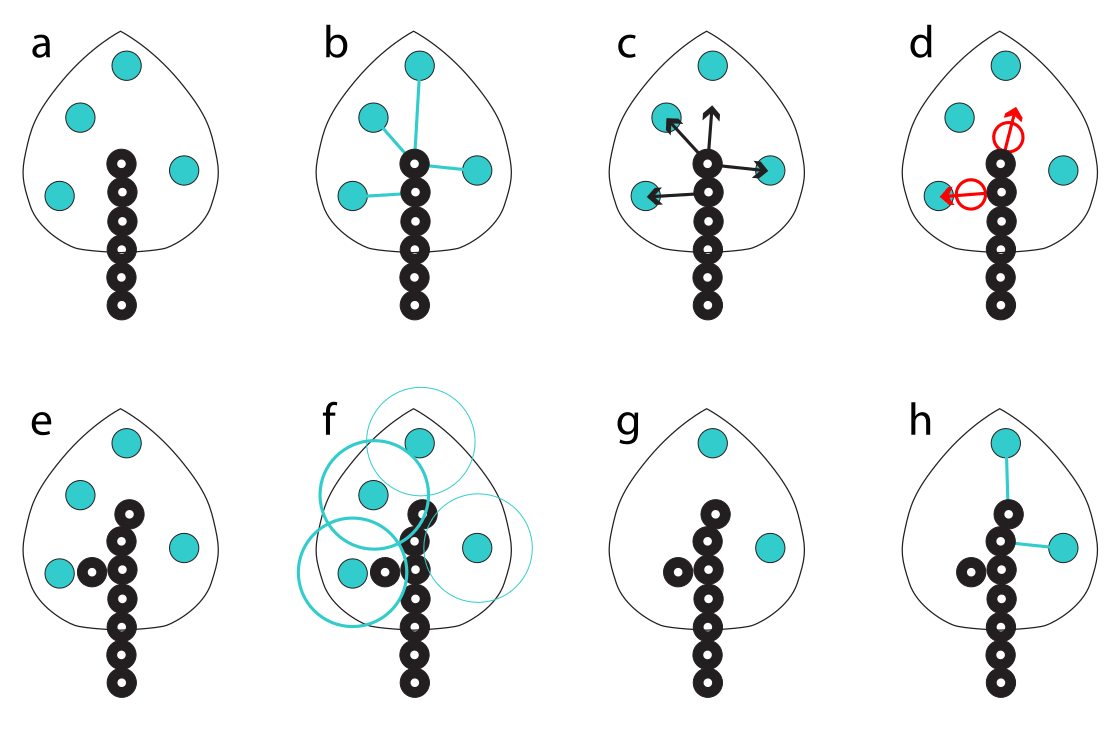
\includegraphics[width=0.5\textwidth]{obrazky-figures/space-col/space_col_main.png}
    \caption[Iteration of Space Colonization algorithm]{Sequence showing an iteration of the Space Colonization algorithm. Black circles denote nodes of the tree structure. Gray dots are attraction points.\footnotemark}
    \label{fig:space-col-description}
\end{figure}

\footnotetext{Image taken from an article about Space Colonization algorithm by Runions et al.~\cite{space-colonization}.}

The general function of the space colonization algorithm can be seen in Fig.~\ref{fig:space-col-description} and works as follows:
\begin{enumerate}
  \renewcommand{\labelenumi}{\alph{enumi})}
  \item The iteration begins with 6 tree nodes (black circles) and 4 attraction points (gray dots).
  \item Each attraction point finds its closest node and checks whether it can influence it (radius of influence $d_i$). In this case, all attraction points find nodes that they can influence.
  \item Normalized vectors toward the influencing attraction points are calculated.
  \item The average direction vector for each node is calculated from all its vectors.
  \item New nodes are added at the correct positions calculated with $v' = v  + D\hat{n}$.
  \item Attraction points are checked for proximity to new nodes. Those that are closer to any node than the defined kill distance $d_k$ are to be removed.
  \item Attraction points that were too close to the nodes were removed.
  \item The algorithm continues in a~similar way.
\end{enumerate}

The space colonization algorithm is utilized mainly to generate realistic trees and bushes, where it achieves quite impressive results (see Fig.~\ref{fig:space-col-tree}), especially considering its simplicity and the fact that it utilizes different approaches than previous tree generators, which relied mostly on L-Systems, geometric properties of trees, and others~\cite{space-colonization}.

\begin{figure}[htbp]
    \centering
    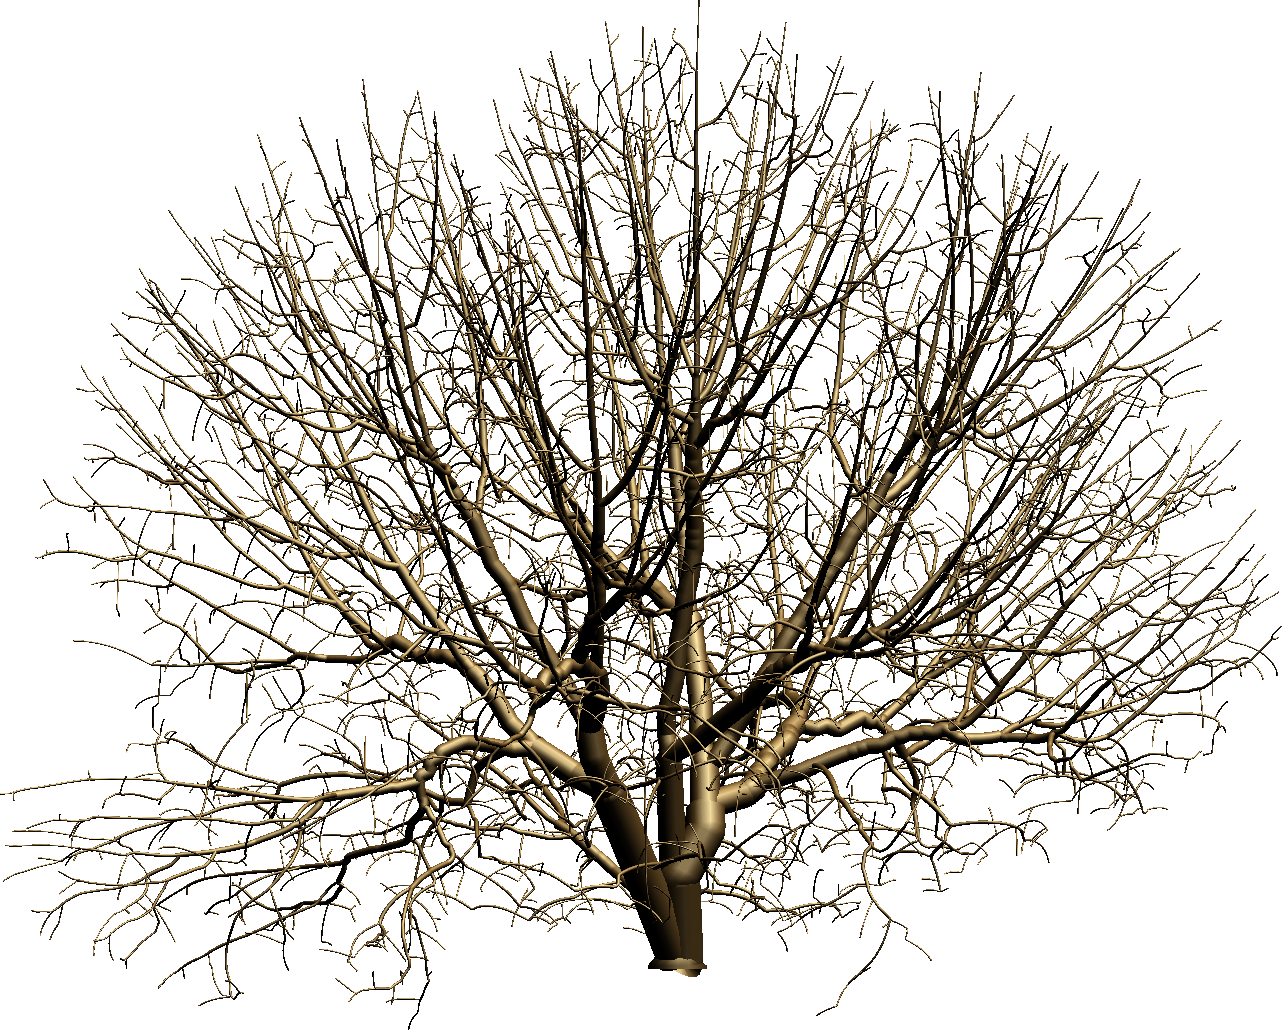
\includegraphics[width=0.5\textwidth]{obrazky-figures/space-col/space-col-example-tree.png}
    \caption[Space colonization - generated tree]{Example tree generated with the Space Colonization algorithm.\footnotemark}
    \label{fig:space-col-tree}
\end{figure}

\footnotetext{Image taken from an article about Space Colonization algorithm by Runions et al.~\cite{space-colonization}.}

\section{Depression Filling and Sampling Methods}
This section describes two often-used methods in the field of depression filling for digital elevation models (DEM) and uniform sampling in computer imagery, which can be useful for procedural content generation.

\subsection{Priority-Flood Algorithm}\label{priority_flood}
The Priority-Flood algorithm~\cite{priority_flood_barnes} is an efficient method for filling depressions in DEMs. It works by filling the DEM area inward from its edges and uses a~priority queue of cells, ordered by cell height (the lowest height is processed first). Initially, the algorithm inserts all edge cells of the DEM into the priority queue and marks them as processed. Then it continues to pop cells out of the priority queue. Each popped cell iterates over its neighbors. If the neighbor cell has not yet been processed, its elevation is set to the maximum of its current height and the current expanding cell's height, and it is placed in the priority queue. This ensures that the depressions are filled and that the region always spills toward its edges. The algorithm is formally defined in Alg.~\ref{alg:priority_flood}.



\begin{algorithm}
\caption{Priority-Flood~\cite{priority_flood_barnes}}\label{alg:priority_flood}
\begin{algorithmic}[1]
\Require $\mathit{DEM}$
\State Let $\mathit{PQ}$ be a~priority queue
\State Let $\mathit{DONE}$ be of the same size as $\mathit{DEM}$ and let it contain all processed cells
\State Let $\mathit{DONE}$ be initialized to \textsc{false}
\ForAll{$c$ on the edges of $\mathit{DEM}$}
\State Push $c$ in $\mathit{PQ}$ with priority $\mathit{DEM}\left(c\right)$
\State $\mathit{DONE}\left(c\right) \gets$ \textsc{true}
\EndFor
\While{$\mathit{PQ}$ is not empty}
\State $c \gets$ \textsc{pop}$\left(\mathit{PQ}\right)$
\ForAll{neighbors $n$ of $c$}
\If{$\mathit{DONE}\left(n\right)$}
\State $\mathbf{continue}$
\EndIf
\State $\mathit{DEM}\left(n\right) \gets$ \textsc{max}$\left(\mathit{DEM}\left(n\right), \mathit{DEM}\left(c\right)\right)$
\State $\mathit{DONE}\left(n\right) \gets$ \textsc{true}
\State Push $n$ in $\mathit{PQ}$ with priority $\mathit{DEM}\left(n\right)$
\EndFor
\EndWhile

\end{algorithmic}
\end{algorithm}


Apart from its use in geographic DEM processing~\cite{priority_flood_barnes}, it could also be used as an effect on procedurally generated terrain in games to create flat sections or lakes.

\subsection{Poisson Disk Sampling}
Poisson disk sampling~\cite{stochastic_sampling_cook} is a~sampling technique that generates random points with the restriction that no two points are placed closer together than a~defined distance. The comparison between uniform random and Poisson disk sampling can be seen in Fig.~\ref{fig:random_poisson_comparison}. Robert Bridson~\cite{fast_poisson_disc_sampling_bridson} published a~possible implementation.

\begin{figure}[htbp]
    \centering
    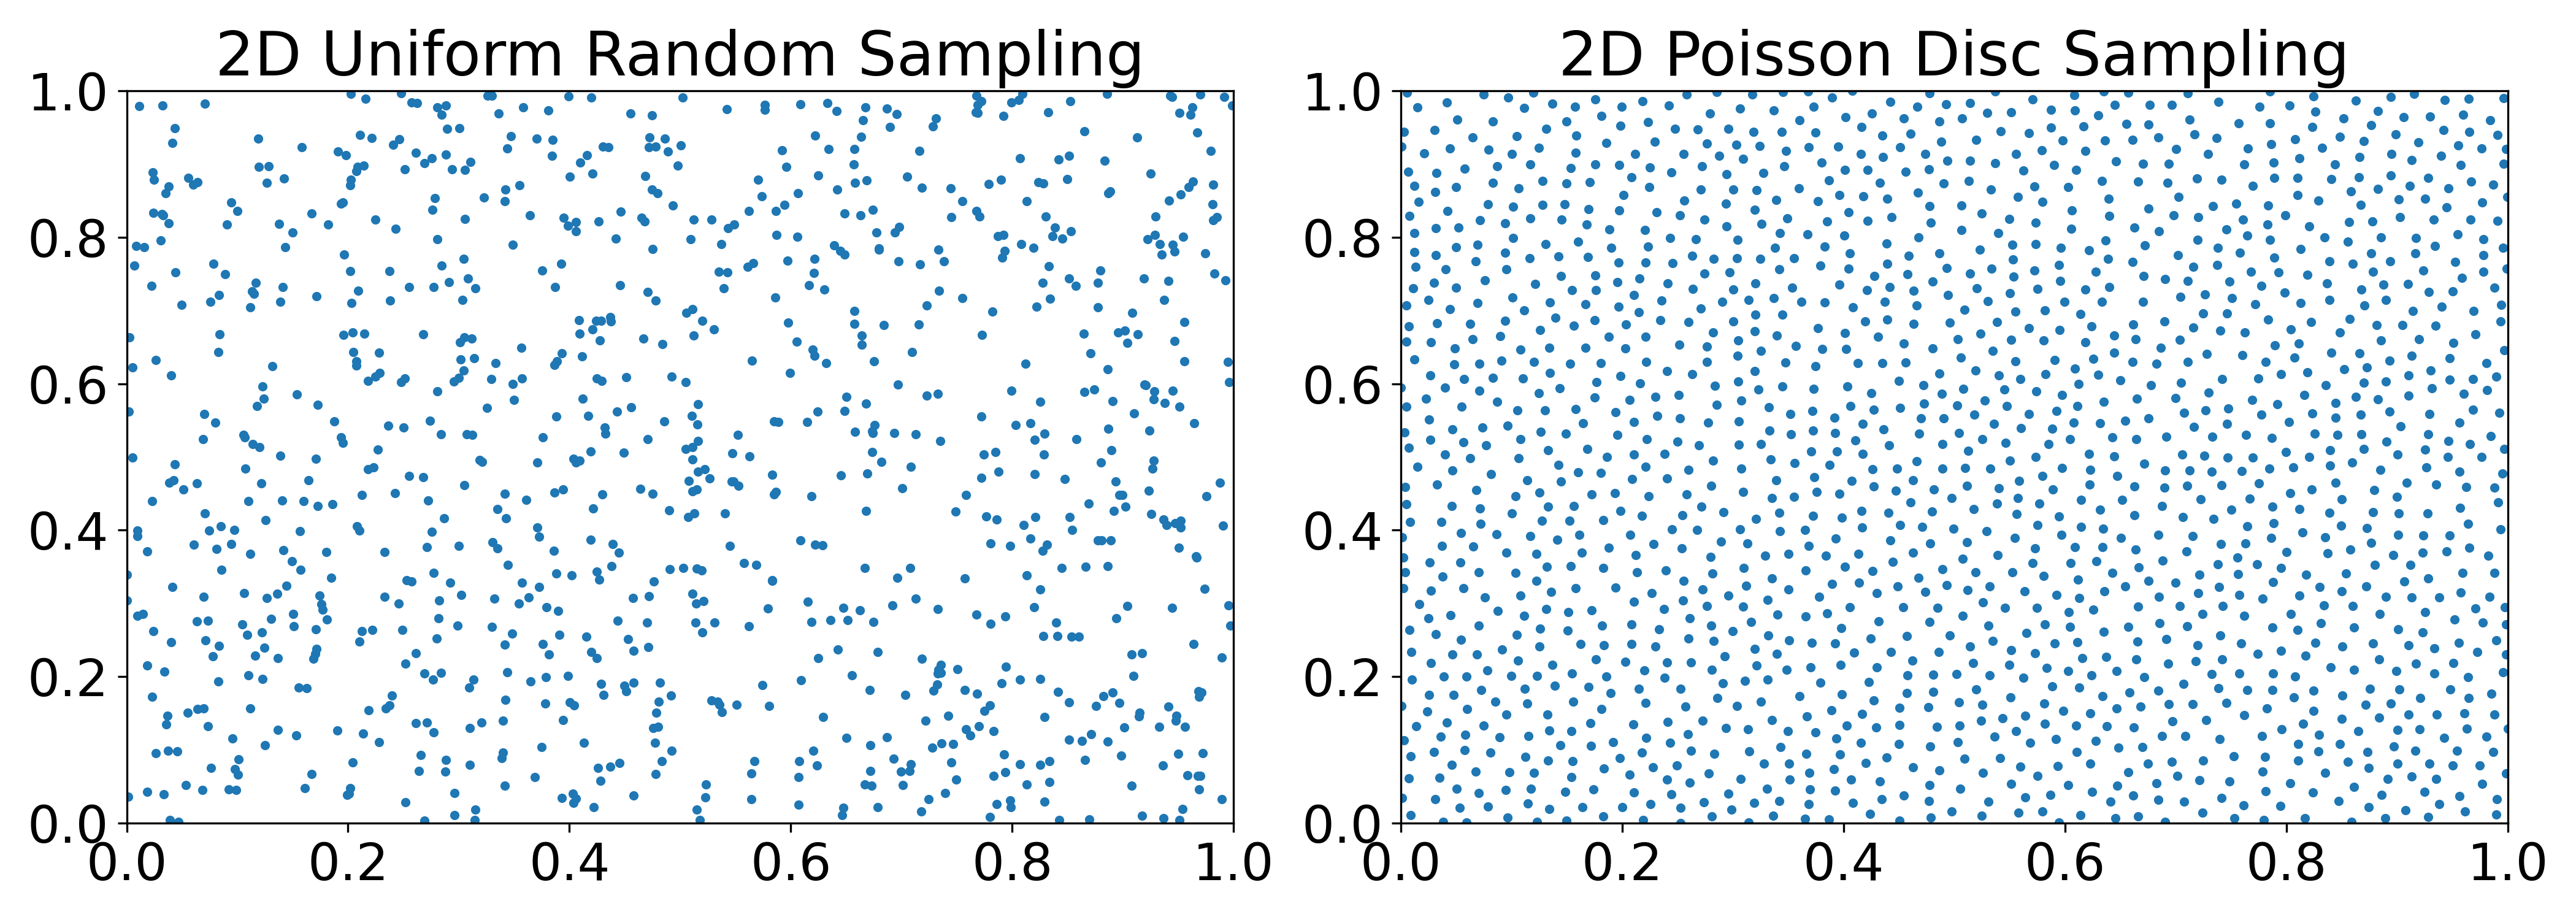
\includegraphics[width=0.8\textwidth]{obrazky-figures/random_poisson_comparison.png}
    \caption[Random - Poisson Comparison]{Comparison of uniform random sampling and Poisson disk sampling for placement of 1000 points on a~2D grid.}
    \label{fig:random_poisson_comparison}
\end{figure}

Poisson disk sampling can be used in procedural content generation to generate natural placements for repeating features, such as plants or grass~\cite{proc_gen_survey_mdpi}.



%%%%%%%%%%%%%%%%%%%%%%%%%%%%%%
% TECHNICAL STUFF FOR VOXELS
%%%%%%%%%%%%%%%%%%%%%%%%%%%%%%
\chapter{Technical Solutions for Voxel Worlds}\label{tech-sol-voxel-worlds}
This chapter discusses the technical solutions required for a~runtime-modifiable representation of 3D space. Mostly from the perspective of cubic sandbox voxel games, where each voxel represents a~discrete cube of 3D space located in a~3D integer grid (see Fig.~\ref{fig:voxel_space_visualization}), usually representing one of the defined block types. The formal mapping function for a~given 3D coordinate to a~defined block type can be seen in Eq.~\ref{eq:discrete_voxels}. The chapter discusses structures for storing voxel information, approaches for voxelization and interaction with voxel data, and methods for their visualization.

\begin{equation}\label{eq:discrete_voxels}
    f\left(x, y, z\right) \in \left\{\mathit{AIR}, \mathit{STONE}, \mathit{WOOD}, \mathit{WATER}, \ldots\right\}
\end{equation}

\begin{figure}[htbp]
    \centering
    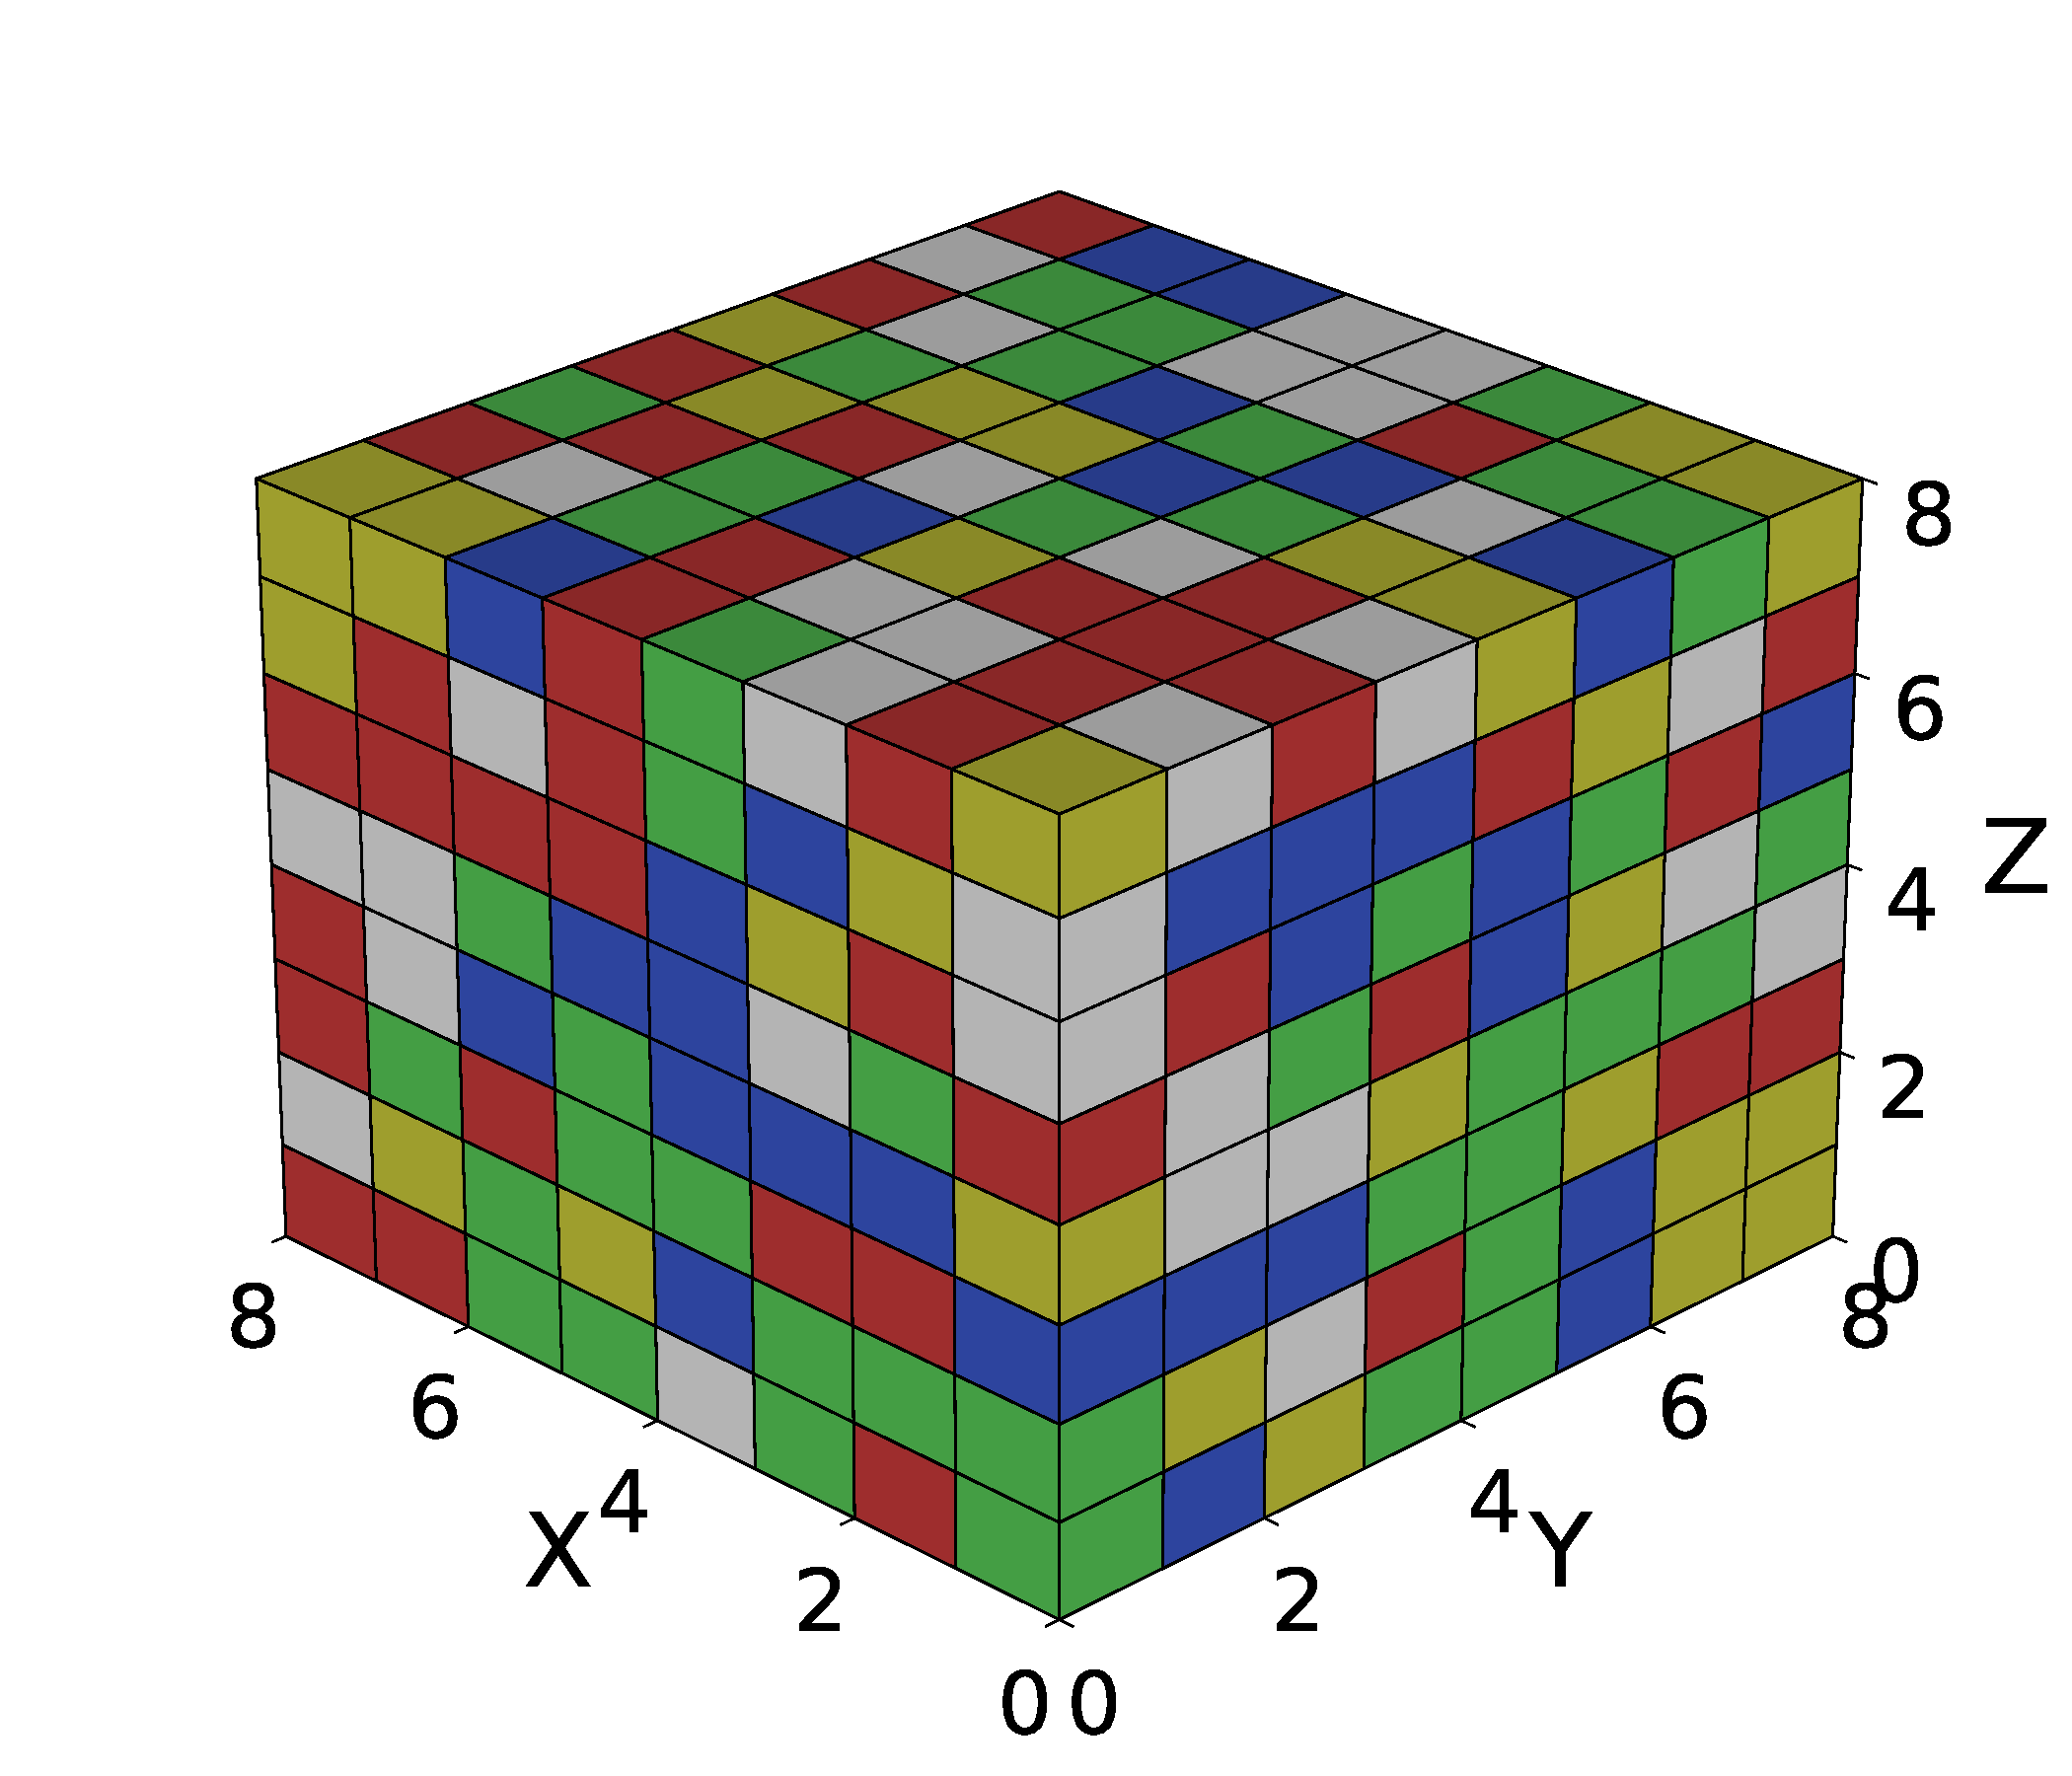
\includegraphics[width=0.45\textwidth]{obrazky-figures/voxel_grid.pdf}
    \caption[Visualization of 3D voxel grid.]{Visualization of 3D voxel grid.}
    \label{fig:voxel_space_visualization}
\end{figure}

\section{Efficient In-Memory World Representation}

There are various methods~\cite{voxel_algo_data_structs} for the internal representation of voxel information, each with its own area of application and strengths and weaknesses. As voxels represent a~gridded 3D space, the simplest solution to store voxel information is to use 3D arrays~\cite{voxel_algo_data_structs} with integer indexing, where each cell stores the block type that occupies it. 

This approach also allows fast searches and straightforward voxel management. However, it is not suitable for large voxel environments or for those with very small voxels, as memory requirements grow rapidly with the size and detail level. Voxel environments are also usually populated sparsely~\cite{voxel_algo_data_structs}, so a~regular grid does not make sense. In addition, this approach does not allow effective queries and editing of large spatial areas, making the implementation of level-of-detail mechanisms and ray casting less efficient~\cite{voxel_algo_data_structs}. A~viable solution that addresses the majority of these issues is a sparse voxel octree structure.

\subsection{Sparse Voxel Octrees}\label{svos}
Sparse voxel octrees (SVO)~\cite{voxel_algo_data_structs} are octet-tree structures of nodes representing the voxel space, where each node of the tree structure represents a~cube of space and can be expanded into 8~higher-resolution child nodes, each of which represents a~sub-cube of its parent. This allows the octet structure to efficiently store sparse data, as areas with a~high amount of detail can be represented by deeper levels of the tree, while areas with the same properties can be collapsed to shallower levels, thus saving memory, as can be seen in Fig.~\ref{fig:voxel_regular_sparse_voxel_octrees_diff}, in contrast to regular grid voxel structures.

\begin{figure}[htbp]
    \centering
    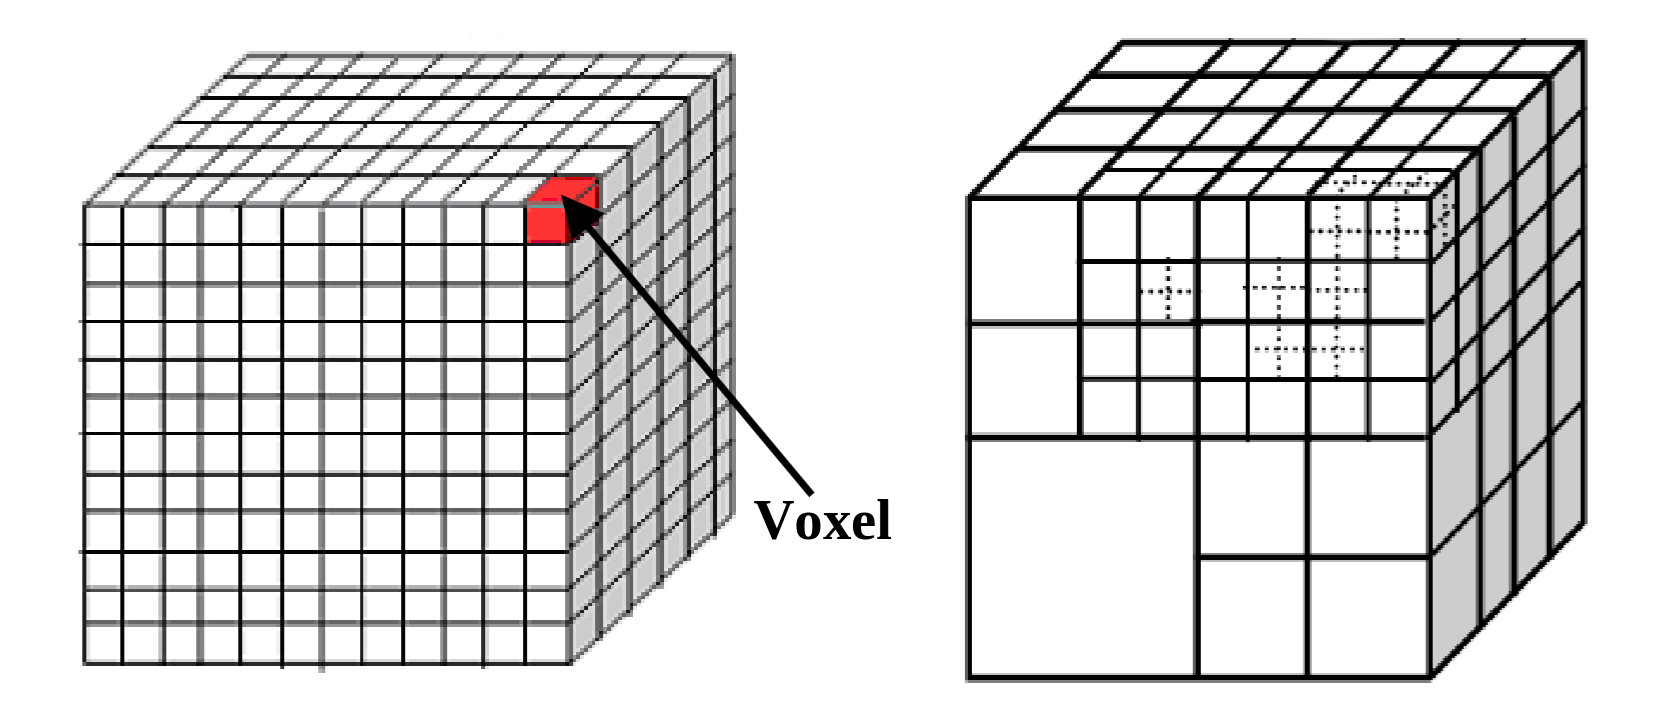
\includegraphics[width=0.6\textwidth]{obrazky-figures/voxel_sparse_voxel_octree.png}
    \caption[Voxel and Sparse Voxel Octree Grid]{Visualization of regular voxel grid (left) and sparse voxel octrees (right).\footnotemark}
    \label{fig:voxel_regular_sparse_voxel_octrees_diff}
\end{figure}
\footnotetext{Image source: \href{https://doi.org/10.1109/NGNS.2014.6990252}{\texttt{doi.org/10.1109/NGNS.2014.6990252}}}

SVOs not only efficiently store sparse voxel data but also enable efficient traversal, processing, and modification of voxel information with variable-sized queries~\cite{voxel_algo_data_structs}, which is beneficial for ray casting and enables efficient implementation of level-of-detail mechanisms.

On the other hand, SVOs have higher processing overhead than regular grid structures when deep levels of the tree are queried or modified, and the overhead of necessary pointers can be considerable if there are only a~few collapsible areas.


\subsection{Chunk Systems}\label{chunk_systems}

Sandbox voxel games usually feature very large worlds, often pseudo-infinite and procedurally generated. Modern Minecraft\footnote{Minecraft Wikipedia world boundary article: \href{https://minecraft.wiki/w/World_boundary}{\texttt{minecraft.wiki/w/World\_boundary}}} versions feature a~world with boundaries at $\pm$ \numprint{30000000} meters in X~and Z~dimensions. Such large worlds cannot be stored in memory simultaneously, no matter how many optimizations are applied.

The solution for this is to use chunk systems~\cite{bloxel_bachelor_thesis, aokana_voxel_engine}, which divide the world into small regions (chunks) that can be loaded and unloaded on demand. Typically, only a~small number of such chunks are active at the same time, usually covering only the necessary circular or rectangular area around the player that they can see. The rest of the chunks are procedurally generated when requested or loaded from disk, where they are usually stored in a~compact, compressed format using algorithms such as Run-length encoding~\cite{voxel_optimization_rle}.


\section{Voxelization and Interaction with Voxel Environments}
There are various voxelization algorithms for converting 2D and 3D primitives, as well as polygonal models, and 3D scans into a voxel representation~\cite{voxel_algo_data_structs}. These methods include solutions for points, lines, curves, polygonal geometry, and more. However, when it comes to the direct generation of voxel environments in sandbox voxel games, especially when the generation process is entirely procedural and does not utilize any 3D models that were created in advance, many of the complex methods are not necessary, and the remaining ones are targeted at the voxelization of primitives and simple 3D objects such as points, lines, curves, cubes, and spheres.

\subsection{Voxelization of Points, Cubes and Spheres}
The simplest primitive to voxelize is a~single point. A~typical process of point voxelization~\cite{voxel_algo_data_structs} includes translation of its coordinates to the voxel space, then division of the point coordinates by voxel size. After this, the point can be recorded in the voxel structure at its integer coordinates.

When the voxel space is directly edited by the procedural generation pipeline, it might be beneficial to use the same coordinate system and operation sizes so that these translation steps can be omitted.

Simple methods for voxelizing cubes (cuboids) and spheres can be built on top of point-based voxelization. In this manner, a~basic implementation of cube or cuboid voxelization would first calculate the corner points and map them to voxel-space coordinates, as for a~point. The algorithm would then loop within the 3D space defined by the corner points, advancing in each dimension by a~defined voxel size, and each sampled point would be recorded in the voxel structure.

The voxelization of a~sphere can be done similarly. The cubic bounding box of a~sphere can be created depending on its radius. Then the algorithm would be similar, but only points within the radius of the sphere would be recorded in the voxel structure. This check can be performed with Eq.~\ref{eq:sphere_distance_check}, where $x$, $y$, and $z$ denote the current sampled point, $x_0$, $y_0$, and $z_0$ denote the center of the sphere, and $r$ is the radius of the sphere.

\begin{equation}\label{eq:sphere_distance_check}
    (x - x_0)^2 + (y - y_0)^2 + (z - z_0)^2 \leq r^2
\end{equation}


\subsection{Real Line Voxelization Algorithm}\label{rlv}
Real line voxelization (RLV)~\cite{real_line_voxelization, voxel_algo_data_structs} is an efficient algorithm for the voxelization of lines, often used in ray casting, both for visualization of voxel information~\cite{real_line_voxelization} and implementation of real-time interaction of voxel game players with the voxel environment~\cite{bloxel_bachelor_thesis}.

This algorithm~\cite{real_line_voxelization, voxel_algo_data_structs} traverses a~voxel grid iteratively by stepping to the next voxel along the direction of the line. At each step, it determines which axis-aligned voxel boundary will be intersected next by comparing parametric distances along the line. The voxel corresponding to the smallest such distance is selected, and the traversal proceeds into that voxel. The algorithm is quite efficient, as each step requires only a~handful of arithmetic operations and comparisons.

\subsection{Bézier Curves and De Casteljau's Algorithm}\label{bezier_de_casteljau_algo}
Sometimes, it is necessary to work with curves and thus voxelize them. One of the commonly used curve representations in computer graphics is a~Bézier curve~\cite{bezier_curves}.

For the evaluation of a~specific point $t \in \left[0, 1\right]$ that lies on the Bézier curve, de Casteljau's algorithm~\cite{bezier_curves} can be utilized. The algorithm recursively uses linear interpolation to evaluate the point. It starts with computing linear interpolations between each pair of neighboring control points at parameter $t$. The newly obtained points form a~new set of control points. Linear interpolations are then performed between each pair of neighboring points at parameter $t$. The process is repeated recursively until only a~single point remains. This final point is the result of the evaluation, and its position corresponds to the location on the Bézier curve at parameter $t$.

\begin{figure}[htbp]
    \centering
    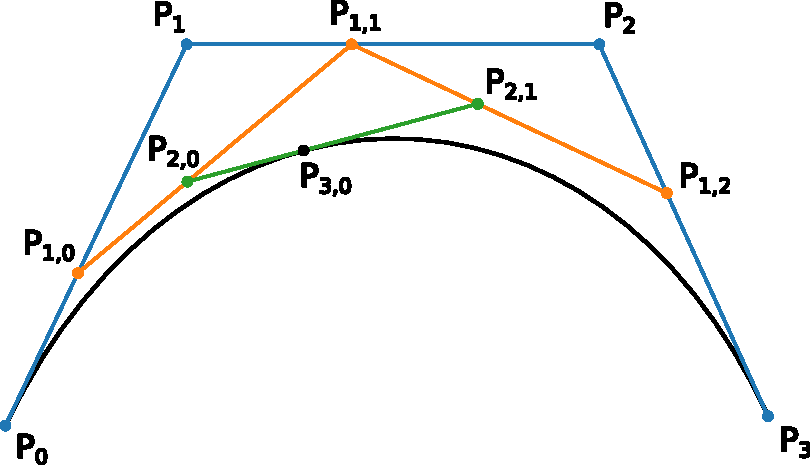
\includegraphics[width=0.45\textwidth]{obrazky-figures/bezier_curve_de_casteljau_visualization.pdf}
    \caption[Visualization of de Casteljau's algorithm]{Visualization of de Casteljau's algorithm for a~Bézier curve with 4~control points.}
    \label{fig:de_castlejau_visualization}
\end{figure}

The visualization of de Casteljau's algorithm for evaluation at $ t = 2 / 5$ can be seen in Fig.~\ref{fig:de_castlejau_visualization}. Points $P_0$, $P_1$, $P_2$, and $P_3$ are the control points of the Bézier curve. Points $P_{1,0}$, $P_{1,1}$, and $P_{1,2}$ are the new control points at the interpolated positions from the first iteration, points $P_{2,0}$, and $P_{2,1}$ from the second, and point $P_{3,0}$ is the resulting evaluated point on the Bézier curve.

When it comes to the voxelization of such a~curve, the points evaluated by de Casteljau's algorithm could be either voxelized directly with the point voxelization mentioned above or used as positions for voxelization of spheres if the curve should have a~specific width.

\section{Visualization of Voxel Worlds}

There are numerous visualization methods for rendering voxel information~\cite{volume_rendering_techniques, voxels_polygons_voxel_rendering_comparison}, usually divided into two main categories, which are direct and indirect volume rendering~\cite{volume_rendering_techniques, voxels_polygons_voxel_rendering_comparison}. Each has its strengths and drawbacks. Techniques suitable for voxel games are discussed in detail.

\subsection{Direct Volume Rendering}\label{dvr}

Direct volume rendering (DVR) directly uses voxel data for visualization without preprocessing steps such as extraction of (iso)surfaces~\cite{real_time_volume_graphics}. This visualization usually occurs through the evaluation of an optical model that describes volume characteristics~\cite{real_time_volume_graphics}, or by real-time visualization of ray intersections with surfaces in the voxel environment~\cite{ray_casting_iso_surface_rendering}. The methods most suitable for rendering sandbox voxel games include (iso)surface ray casting and ray casting.

\subsubsection{Surface Ray Casting}
Surface ray casting~\cite{ray_casting_iso_surface_rendering, real_time_ray_casting_isosurfaces}, or in the case of non-discrete density-based voxel environments, isosurface ray casting, is a~real-time DVR rendering method. It uses rays cast from each pixel of the screen space into the voxel scene, which travel through non-solid voxels until they intersect with a~solid voxel or travel too far. Or in the case of isosurface ray casting, until a~specified density threshold is crossed. This is usually done by iteratively traversing the voxel space using algorithms such as RLV~\cite{voxel_algo_data_structs, real_line_voxelization}, and sampling the voxel environment. In contrast to regular ray casting, the values of sampled voxels are used only to determine whether the ray continues or intersects with a~solid voxel. In the latter case, the traversal stops, and the pixel is shaded based on the voxel's type. A~visualization of the method is shown on the left side of Fig.~\ref{fig:ray_casting_collage}.


\begin{figure}[t]
    \centering
    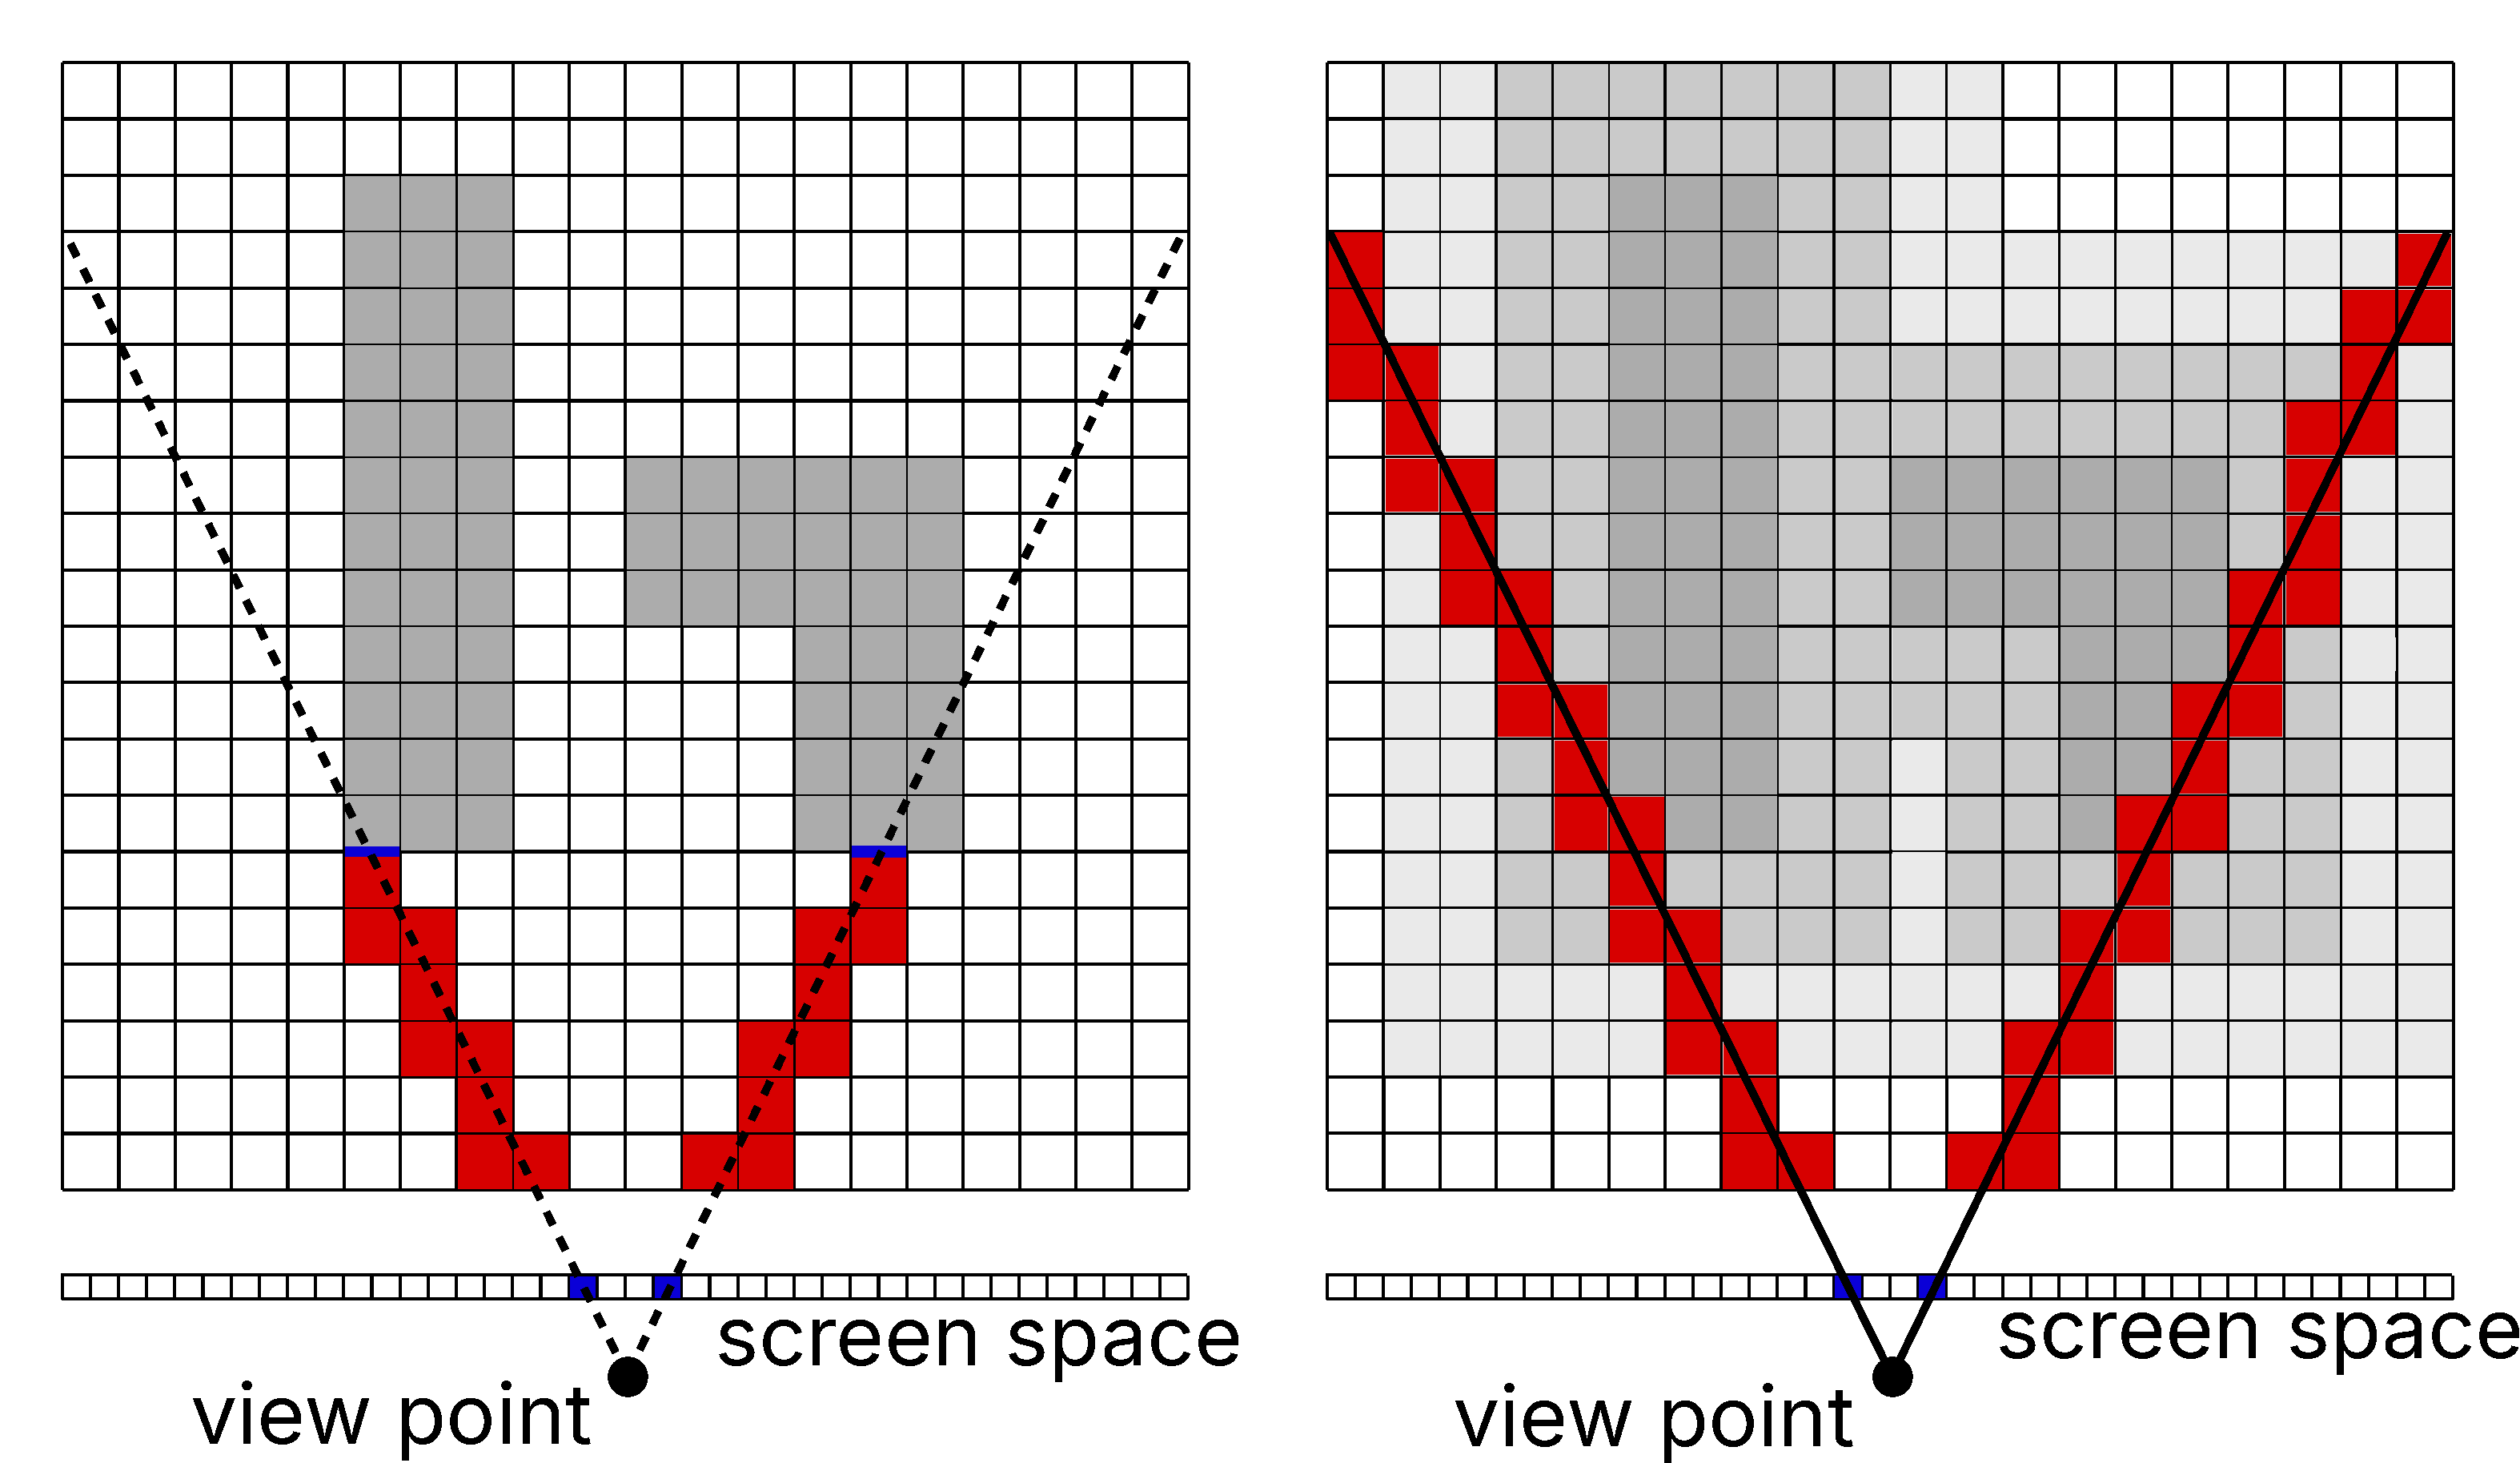
\includegraphics[width=0.60\textwidth]{obrazky-figures/ray_casting_collage.pdf}
    \caption[Ray Casting Comparisons]{Comparison of surface ray cast on the left and regular ray cast on the right. Gray cells denote voxels. Red cells represent cells visited along the ray, while blue cells in the screen space visualize the starting points of the ray casts. Their values depend on the intersected cell in the case of surface ray cast or the calculated value for regular ray cast.}
    \label{fig:ray_casting_collage}
\end{figure}


\subsubsection{Ray Casting}
Ray casting uses the principle of casting rays from each pixel in the screen space through a~density-based voxel volume~\cite{real_time_volume_graphics, volume_rendering_techniques, voxels_polygons_voxel_rendering_comparison}. The typical approach involves sampling the voxel volume density data along the ray's path through the voxel scene. The data accumulated along the ray path are then used to compose the final pixel color values. It represents a~numerical solution of the volume rendering integral in Eq~\ref{eq:volume_rendering_equation}, which calculates the total amount of radiant energy $C$~that reaches the viewing point as an integral over a~set of sampled points along the ray~\cite{real_time_volume_graphics}. Visualization of this method can be seen on the right side of Fig.~\ref{fig:ray_casting_collage}. This approach allows visualization of translucency and various volumetric effects that are not entirely possible with surface-based indirect volume rendering~\cite{real_time_volume_graphics} or with surface ray casting.

\begin{equation}\label{eq:volume_rendering_equation}
    C = \int_0^\infty{c\left(t\right)\cdot e^{-\tau\left(0, t\right)} dt}
\end{equation}

\subsection{Indirect Volume Rendering}\label{ivr_rendering_voxels}

In contrast to DVR, indirect volume rendering (IVR) methods preprocess voxel information to extract polygonal surface geometry, which is then displayed using the general GPU pipeline~\cite{volume_rendering_techniques, voxels_polygons_voxel_rendering_comparison}. The IVR methods commonly used in voxel games could be split into two main categories based on the type of extracted surfaces. These are smooth surfaces and cube-styled surfaces. Smooth surfaces are often generated using methods such as Marching Cubes~\cite{marching_cubes} or Dual Contouring\footnote{0 FPS Blog post:~\href{https://0fps.net/2012/07/12/smooth-voxel-terrain-part-2/}{\texttt{0fps.net/2012/07/12/smooth-voxel-terrain-part-2}}}~\cite{0fpsblog}, while cube-styled surface generation uses simple methods that directly represent voxels as cubes~\cite{simplified_voxel_games}.


\begin{figure}[t]
    \centering
    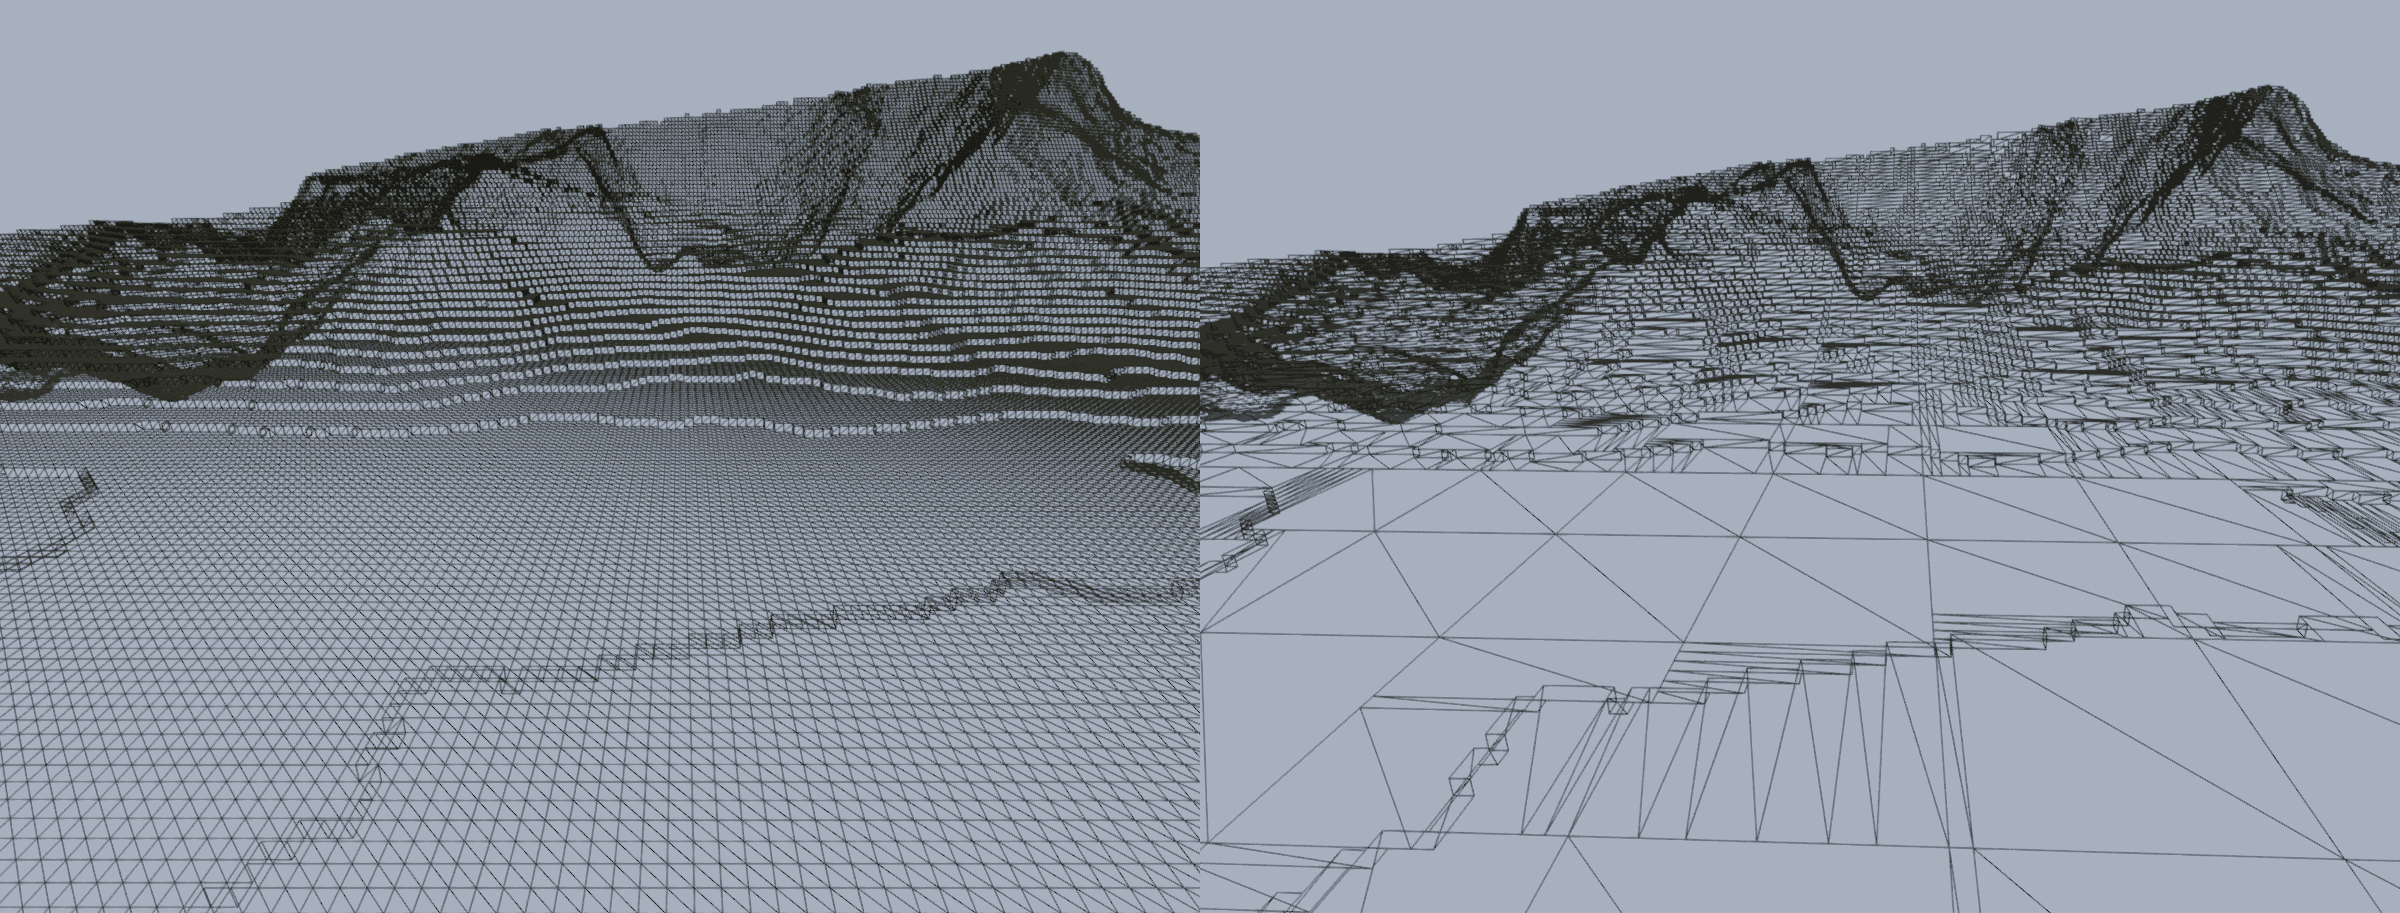
\includegraphics[width=1.0\textwidth]{obrazky-figures/meshing_comparison.png}
    \caption[Naive vs Greedy Meshing]{Wireframe of a~voxel scene generated with naive cubical surface extraction on the left, and greedy meshing algorithm on the right.}
    \label{fig:naive_greedy_meshing_comparison}
\end{figure}

\subsubsection{Naive Cubical Surface Extraction}
Sandbox voxel games, such as Minecraft, use a~cubic style to visualize their discrete, block-based voxel environments~\cite{simplified_voxel_games}. The simplest approach to generating such surfaces is to directly map the cubical voxel space to cubes, then generate cube faces that lie on the edges between solid and non-solid voxels.

This can be done by iterating over the voxels and checking all neighboring voxels for each of the 6~faces of the current voxel. As each face is a~quad that requires 2~triangles, a~lone voxel cube would need 12 triangles in total. This is a~simple approach to implement, but it produces an overly complex geometry, as is shown on the left side of Fig.~\ref{fig:naive_greedy_meshing_comparison}. 


\subsubsection{Cubical Surface Extraction with Greedy Meshing}
As can be seen on the left side of Fig.~\ref{fig:naive_greedy_meshing_comparison}, there are many neighboring faces on the same planes that could be merged into larger quads, and thus rendering of such a~scene would require significantly less geometry. This is the goal of the greedy meshing algorithm\footnote{0~FPS~Blog posts:~\href{https://0fps.net/2012/06/30/meshing-in-a-minecraft-game/}{\texttt{0fps.net/2012/06/30/meshing-in-a-minecraft-game}} and:~\href{https://0fps.net/2012/07/07/meshing-minecraft-part-2/}{\texttt{0fps.net/2012/07/07 /meshing-minecraft-part-2}}}~\cite{0fpsblog}, which generates the surface geometry of the voxel environment with quads made by merging adjacent faces of the same voxel type and located on the same plane.


The algorithm works on slices of the voxel space that are perpendicular to the normals of 6 cube faces. Each slice then becomes a~2D optimization problem of finding surface faces and merging them into larger quads when possible. Surface faces can be merged with their neighbors as long as all of them have the same type and together form a~quad. This can be done by iteratively extending the width and height of the current quad until it is as wide and tall as possible. The resulting merged quads then compose the geometry of the extracted surface. The optimized wireframe is shown on the right side of Fig.~\ref{fig:naive_greedy_meshing_comparison}.


\subsection{DVR and IVR Comparison}
DVR methods and specifically ray casting techniques can lead to better performance compared to IVR methods, as their performance depends mainly on the size of the screen space, while in IVR methods, their time costs for surface extraction and the resulting polygon counts increase with the complexity of the scene~\cite{voxels_polygons_voxel_rendering_comparison}. On the other hand, IVR methods are useful for rendering simple scenes and those that change infrequently. Optimized methods, such as the greedy meshing algorithm, can produce simpler geometry, but these come with a~higher extraction cost.



%%%%%%%%%%%%%%%%%%%%%%%%%%%%%%
% World Generator Design
%%%%%%%%%%%%%%%%%%%%%%%%%%%%%%
\chapter{World Generator Design}\label{world-gen-design}

In this chapter, inspirations, along with goals and objectives for a~fully procedural world generator, are discussed, and a~design for a~complex world-generation system suitable for large-scale sandbox voxel games and demos is proposed.


\section{World Generator Inspiration and Objectives}

There are two main reasons why a~procedural generator for sandbox voxel games was chosen as the topic of this thesis. The first is that sandbox voxel games are highly suitable for the use of PCG methods, enabling the application of various procedural generation techniques, including their testing and extension of their capabilities. The second is the overall gameplay possibilities this genre offers, especially regarding player creativity and exploration options, as discussed in Section~\ref{sandbox-voxel-games}.

\subsection{Inspiration from Existing Games}

The sandbox voxel games Minecraft and Lay of the Land were the biggest inspirations for the design and implementation. Minecraft inspired this thesis with its vast, yet diverse, detailed, and dynamic procedurally generated world environments, featuring varied terrain, underground cave networks, and a~wide range of vegetation and decorations.

At the same time, the game Lay of the Land shows that this is also possible with considerably higher voxel detail, which can not only improve visuals and gameplay features, but allows the game to generate and use even more detailed environments, with semi-realistically looking vegetation and other decorations such as rocks, fallen trees, or in the case of the underground, stalactites, veins, and more. The game Lay of the Land also influenced this thesis by streamlining it to focus on the landscape and natural environments, such as forests and meadows, leaving behind other non-natural elements.


\subsection{Specifications of Goals and Objectives}
The main goal is to create a~deterministic procedural world environment generator capable of generating large, pseudo-infinite voxel worlds with high voxel detail (voxel size around $1/16$~m) and a~focus on landscapes and natural environments. The generated environments should be semi-realistic and densely populated with natural features, such as vegetation and small decorations. They should feature diverse terrain, biomes, and water systems, as well as underground cave systems. The generated environments should also be game-ready, meaning that they are mostly traversable by a~character, and the landscape should include flatter areas for possible building construction.


\subsubsection{Detailed Objectives}
A~list of detailed objectives follows that the procedural generator must fulfill.

\begin{itemize}
    \item All parts of the environment generator must be deterministic, but they should be configurable and allow a~controllable level of stochastic randomness.
    \item The terrain must be diverse, with mountains, valleys, and flat areas.
    \item The generated environments must contain underground cave systems, with natural decorations and water features. These cave systems must be at least partially reachable from the surface.
    \item The environment must contain water features, such as lakes and rivers. Lakes should be placed in naturally plausible positions, and rivers should flow downward to lower positions in the landscape.
    \item The environments must contain naturally plausible biomes that control the placement of features such as vegetation, decoration, and snow. The biome classification should be based on realistic properties, such as terrain height and water availability.
    \item The environment must feature vegetation and decorations, including deciduous and coniferous trees, shrubs, bushes, grass, plants, rocks, trunks, and stalactites.
    
\end{itemize}

\section{Procedural Generator Architecture}

Before laying out the overall architecture of the procedural generator for voxel worlds, it is important to reiterate that the proposed generator does not use any pre-generated or hand-made assets. Thus, voxel model generation is a~crucial component, and in this thesis, the generation process is split into two main parts, which are:

\begin{itemize}
    \item The voxel model generator.
    \item The environment generator.
\end{itemize}

As specified by the objectives, the environment generator needs to handle a~complex generation process comprising procedural generation of terrain, underground systems, water systems, biomes, and feature placements. It is obvious that some of these steps depend on others if a~deterministic generation is targeted. For example, it is not possible to place vegetation features before biomes are generated, and biome generation also needs to wait until the terrain and water steps are finished, as it requires terrain and water data. This leads to a~hierarchical generation system with dependencies, as outlined in Fig.~\ref{fig:world_generator_architecture}.

\begin{figure}[t]
    \centering
    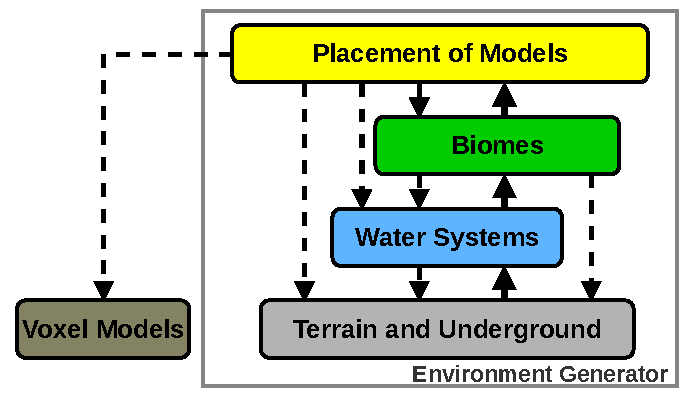
\includegraphics[width=0.6\textwidth]{obrazky-figures/world_generator_bp.pdf}
    \caption[World Generator Architecture]{Diagram showing the architecture of the world generator. Full connections denote the order in which the generation progresses. Dashed lines visualize dependencies.}
    \label{fig:world_generator_architecture}
\end{figure}

These generators are discussed in detail in the following sections, each outlining their goals and designs based on PCG methods such as pseudo-random number generators, procedural noise, custom solutions, and others.

\subsubsection{World Generator Parameters}
To fulfill the outlined objectives of determinism, configurability, and controllable stochastic randomness, the generator and all its components use a~shared seed and their own specific parameters. The seed is used to initialize PRNGs and procedural noise functions, and the component-specific parameters further parameterize the world generator. As the only sources of randomness in the whole generator system are procedural noise functions and PRNGs sharing the same seed, the results of the world generator are the same as long as the seed and component-specific parameters are the same, thus ensuring determinism.


\section{Generator of Voxel Models}\label{voxel_model_generation_design}
The voxel model generator needs to procedurally generate all necessary models, which the environment generator can later place in the world. Its main goal is to produce a~set of assets that look semi-realistic, similar to those in the game Lay of the Land. The methods used should be appropriate for voxelization with the smallest details around $1/16$~m.

The types of models that need to be generated are deciduous and coniferous trees, shrubs, bushes, grass, plants, water plants, fallen trunks, rocks, and stalactites.

There are many possible PCG methods that can be used for the generation of vegetation and other decorations, as discussed in Chapter~\ref{proc-gen-methods}. The following sections propose generators for all the model types mentioned above, mostly utilizing the Space Colonization algorithm for larger vegetation and custom solutions based on basic PCG techniques, such as PRNGs and procedural noise functions, for the rest of them.

\subsection{Generation of Trees and Bushes}\label{generation_trees_bushes}

There are many approaches to generating realistic deciduous and coniferous trees and bushes. Especially suitable methods for the task seem to be L-systems and the Space Colonization algorithm. Of these, the Space Colonization algorithm (see Section~\ref{space-col-algo}) was chosen mainly for its simplicity and the realistic branching structures it creates.

It is important to note that the Space Colonization algorithm does not directly generate trees as models. It only generates realistic-looking branching structures. However, these structures can be easily converted to tree models by calculating segment radii and classifying them into branches and leaves. Radii can be computed in the direction from tips to the tree base as shown in Eq.~\ref {eq:space-col-radii}~\cite{space-colonization}, where $r$~is the radius of a~supporting branch where the branches $r_1$~and $r_2$~meet, and $n$~is a~parameter defining the strength of the effect. The tips usually have defined radii $r_0$.

\begin{equation}
    r^{n} = r_{1}^{n} + r_{2}^{n}
    \label{eq:space-col-radii}
\end{equation}

The possible use of the Space Colonization algorithm for the generation of trees includes the following steps and is shown in Fig.~\ref{fig:space_col_trees_visualization}~\cite{space-colonization}:

\begin{enumerate}
    \item Uniform placement of attraction points within a~defined 3D tree crown shape, such as a~sphere, cylinder, ellipsoid, paraboloid of revolution, cone, or others.
    \item Placement of the starting node. Possibly offset from the bottom of the crown to obtain a~trunk of a~specific height.
    \item Utilization of the Space Colonization algorithm, which is run for up to a~defined set of iterations.
    \item Extraction of the branching structure into a~tree model, calculation of segment radii, and their classification into branch or leaf segments.
\end{enumerate}

\begin{figure}[htbp]
    \centering
    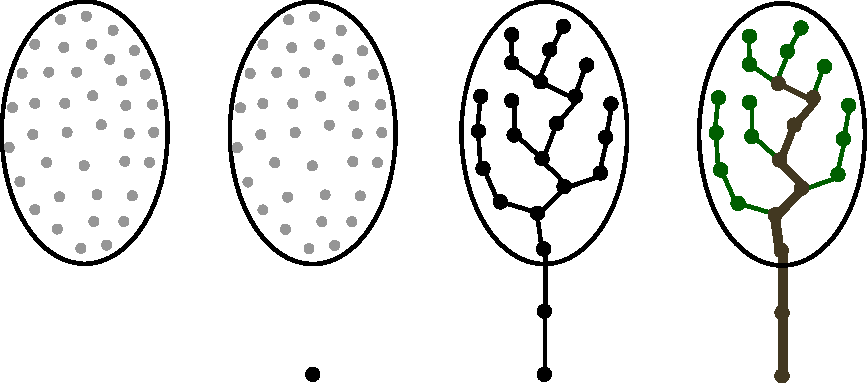
\includegraphics[width=0.48\textwidth]{obrazky-figures/space_colonization_basic_visulalization.pdf}
    \caption[Space Colonization algorithm for generation of trees]{Visualization of the process of generating trees with the help of the Space Colonization algorithm. From left to right, attraction points generation, starting node initialization, the Space Colonization algorithm itself, and tree extraction.}
    \label{fig:space_col_trees_visualization}
\end{figure}

The most important parameters of this method include the total number of attraction points, the 3D shape of the crown (and its proportions), the influence radius, the kill distance, the maximum number of iterations, the segment length, and more.

\subsubsection{Generation of Deciduous Trees}
The Space Colonization algorithm, with attraction points uniformly generated within defined crown shapes, produces good results. However, realistic trees are also influenced by sunlight, and shaded parts of the tree are usually shed. This means that the leaves usually grow on the surface of the tree crown, and the crown's interior is practically hollow, apart from the trunk and supporting branches. This is not possible with uniformly distributed attraction points, as small branches are generated everywhere. However, it can be addressed with adaptive sampling, which distributes more points towards the surface of the crown shape~\cite{space-colonization}, as can be seen in Fig.~\ref{fig:space_col_trees_adaptive_sampling}.

\begin{figure}[htbp]
    \centering
    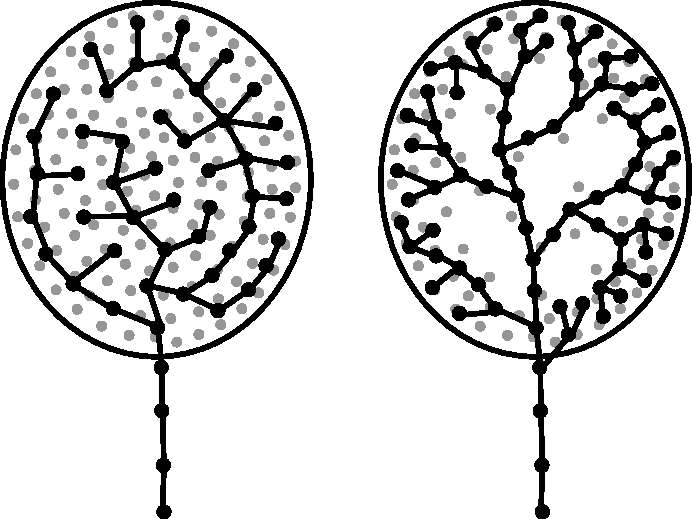
\includegraphics[width=0.35\textwidth]{obrazky-figures/space_colonization_adaptive_sampling.pdf}
    \caption[Space Colonization algorithm with adaptive sampling]{Comparison of uniform sampling of attraction points on the left, and adaptive sampling promoting attraction points towards the crown surface on the right.}
    \label{fig:space_col_trees_adaptive_sampling}
\end{figure}

\subsubsection{Generation of Coniferous Trees}
Another problem is with the growth of some coniferous trees, especially spruces and firs. These trees grow regularly and usually have just a~single main trunk, from which branches grow almost horizontally at discretely spaced vertical levels. This is contrary to the results of the Space Colonization algorithm, which produces less regular and more random patterns.

A solution to this problem is to break down the 3D envelope for generating attraction points into a~set of smaller shapes, such as vertically stacked wedges, with the distance between them exceeding the Space Colonization algorithm's defined influence radius. Thus, the branches will grow in these horizontal wedge sections, similarly to how some conifers grow. The problem and this solution are visualized in Fig.~\ref{fig:space_col_conifers_wedges}.

\begin{figure}[htbp]
    \centering
    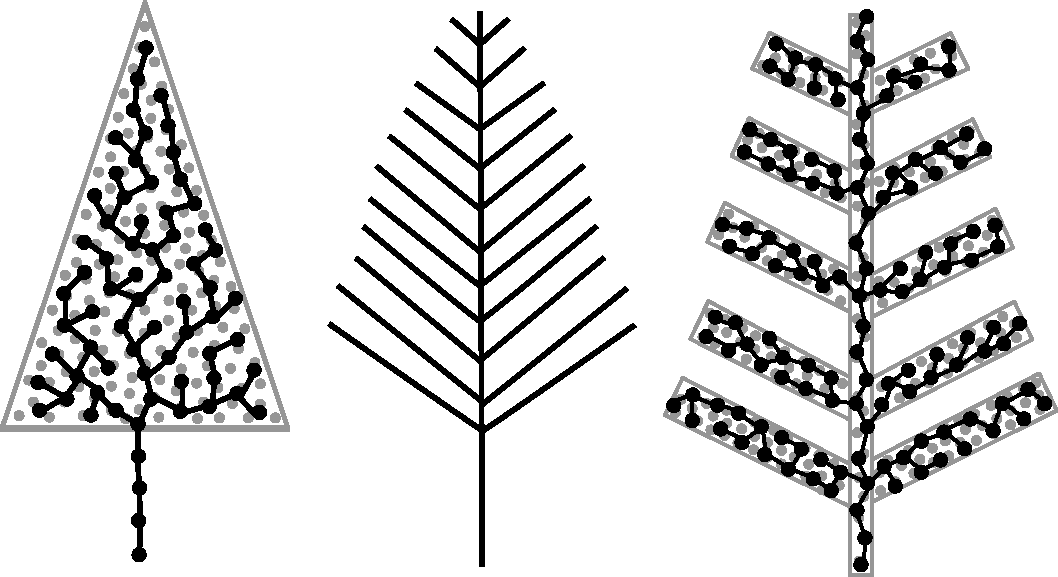
\includegraphics[width=0.46\textwidth]{obrazky-figures/space_colonization_coniferies.pdf}
    \caption[Space Colonization algorithm for coniferies]{Visualization of conifer generation with the Space Colonization algorithm. From left to right, a~conifer generated in a~cone uniformly filled with attraction points, a~simplified spruce, and a~conifer generated with attraction points in vertically stacked wedges.}
    \label{fig:space_col_conifers_wedges}
\end{figure}

\subsubsection{Generation of Shrubs and Bushes}
Shrubs and bushes can also be generated using the Space Colonization algorithm, very similarly to trees. The major difference between bushes and trees is that bushes lack a~visible trunk, and their branches usually sit on the ground, sometimes covering large ground areas. Thus, to generate them, the starting node should be placed at the bottom of the envelope, and perhaps the envelopes should be larger horizontally than vertically.

\subsection{Generation of Small Vegetation}

In this section, a~set of custom generators for small vegetation is proposed. Firstly, the use of L-systems was considered, but it was quickly abandoned in favor of custom generators of simple vegetation models. The main reason is that the smallest detail in voxelization is planned to be around $1/16$~m, which only allows for simplistic vegetation models and thus leaves little room for L-systems to offer advantages. Another reason is that custom solutions can be designed to directly paint into voxel structures, thus simplifying the generation process.

Several simple generators are proposed for generating grass, reeds, small flowers and plants, water lilies, and more. These generators are mostly based on the approximation of observed properties of these plants with basic shapes such as lines, circles, ovals, etc., and the use of PRNGs.

\subsubsection{Approximation of Grass and Simple Flowers with Lines}
Patches of grass can be viewed as sets of grass blades growing from the same small area, each with a~slightly different length and direction. A possible generator could approximate grass blades as lines and utilize PRNGs to randomize generated patches.

\begin{figure}[t]
    \centering
    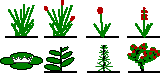
\includegraphics[width=0.65\textwidth]{obrazky-figures/generation_of_simple_plants.pdf}
    \caption[Visualization of Simple Plant Generation]{Visualization of expected results of the mentioned methods. From left to right, top to bottom -- grass, reed or iris, two types of simple flowers, water lily, burdock-like plant, conifer seedling, and a~blooming shrub.}
    \label{fig:simple_plants_expected_results}
\end{figure}

The generation process can start by randomly selecting the total number of blades. Then, each blade would be represented as a~line in parametric form, with a~randomly selected direction of growth and starting point from within a~small circular area of the grass patch.

This approach is also suitable for generating various water plant models, such as reeds or irises, as well as other flowers, including daisies, dandelions, poppies, or bluebells, with only a~small improvement in adding blooms at the ends of the blades or along them.

These methods can be controlled by specifying allowed ranges for randomized properties, such as grass blade counts, blade and leaf lengths, and the dimensions of the circular areas defining the grass patches. The simplified visualization of the expected results is shown in Fig.~\ref{fig:simple_plants_expected_results}.

\subsubsection{Generation of Plants and Flowers with Circular Leaves}
A simple generator of water lilies could randomly place a~number of circular leaves of varying sizes horizontally around the plant's center, then place a~bloom on it.

Plants like burdock feature circular to oval-shaped leaves. Their simple generator could work similarly to water lilies, but instead of placing the leaves in a~single horizontal plane, it would be better to place them around a~small vertical stem at distinct levels.

The important parameters of these methods are similar to those in the previous section, including parameterization of leaf dimensions and the number of leaves. The expected appearance can be seen in Fig.~\ref{fig:simple_plants_expected_results}.



\subsubsection{Generation of Seedlings}
A simple conifer seedling could be generated using the geometric regularity of these trees, as lines growing horizontally at specific vertical levels from the central stem in a~radial pattern. The length of the lines would decrease with each vertical step. This generator could be parameterized by the seedling's height. The expected appearance is shown in Fig.~\ref{fig:simple_plants_expected_results}.

\subsubsection{Generation of Blooming Bushes}
The Space Colonization algorithm was already proposed for generating bushes and shrubs. However, another simple method is proposed here. A typical bush with blooms extends horizontally and branches as it grows upward, with more leaves and blooms in the upper sections. This can be generalized as a~branching structure, in which the likelihood of branches splitting and spawning leaf and bloom patches increases with height. 

In detail, the method would track active tips that can grow, and in each iteration, all active branch tips would be processed, each trying to spread leaf and bloom patches around itself and determine its own fate. It could either continue growing in its direction, split into multiple branches, or end. New branches would randomly select their directions, while always going upward. The plant's height would increase the chances of branch splitting, ending, as well as the formation of leaf and bloom patches. The generation would stop when no branches are active or when the maximum height is reached.

Its parameters should guide the plant's maximum height and the discussed probabilities. Visualization of this method is shown in Fig.~\ref{fig:simple_plants_expected_results}.


\subsection{Generation of Decorations}
There are many types of non-vegetation decorations suitable for placement in landscapes or caverns in voxel environments, but this section only covers voxel model generators for rocks, fallen trunks, and stalactites (and stalagmites).

\subsubsection{Generation of Rocks}
Rocks can take many shapes, from smooth to rugged. A PCG method that could be utilized for their generation is procedural noise, especially multi-octave 3D noise (see Section~\ref{proc_noise_functions}), which can produce various natural patterns. The model can be extracted from the noise using adaptive thresholding based on spherical gradients. The gradient should produce a~minimum at the center of the rock model, with the value increasing as the gradient extends outward. The voxel model of a~rock can then be created by placing stone voxels at positions where the noise value exceeds the gradient value. This can be seen in Fig.~\ref{fig:generation_of_rocks}. The necessary parameters include the requested model size and the noise and gradient configurations.

\begin{figure}[t]
    \centering
    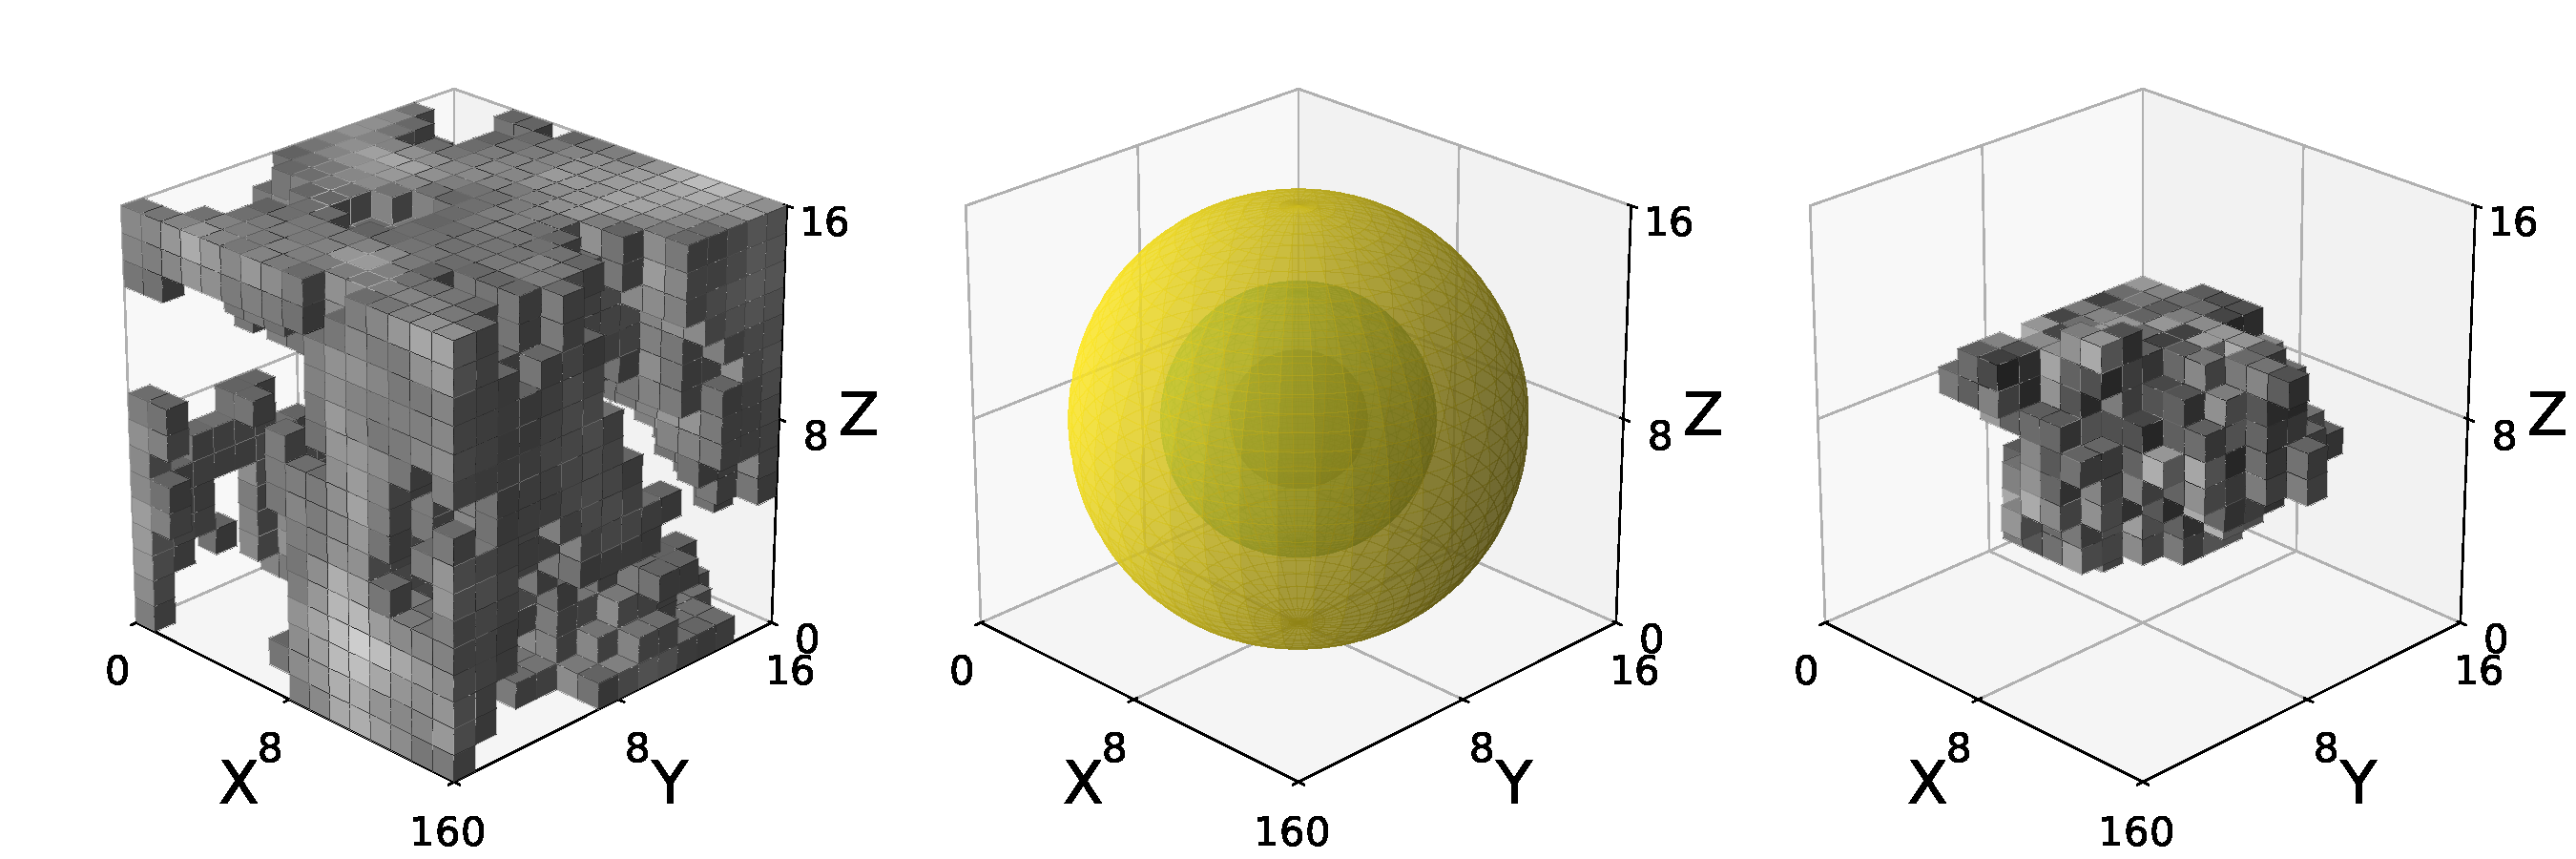
\includegraphics[width=0.95\textwidth]{obrazky-figures/rocks_with_noise.pdf}
    \caption[Visualization of Rock Generation]{Rock generation visualization. From left to right, 3D Perlin noise, spherical gradient, and a~rock model with voxels for spots where noise had values higher than gradient.}
    \label{fig:generation_of_rocks}
\end{figure}

\subsubsection{Generation of Fallen Tree Trunks}
The generation of fallen trunks can be implemented quite easily, using the already-proposed generator for trees in Section~\ref{generation_trees_bushes}. The Space Colonization algorithm can be configured to run for only a~few iterations, producing only the lower parts of the tree. Segments that are too small can be removed, and the model can be transformed into a~lying position, producing a~fallen tree trunk. The parameters of this generator are similar to those of the generator of trees.

\subsubsection{Generation of Stalactites and Stalagmites}
A possible generator of stalactites and stalagmites could approximate their shapes as cones. Another option would be to generate them directly in the voxel space as a~set of spikes (lines) growing up or down from a~horizontal circular area that defines the point of attachment to the cavern surface. Spikes growing from the center of the circle would be the longest, and spikes further away from the center would get progressively shorter. The parameters for this method include the overall size of the stalactite or stalagmite model, the direction of growth, and parameters for randomizing the generation process.

\section{Generator of Terrain Surface and Underground}

The generation of the terrain surface and underground caves is the first step in the environment generation process. Its goal is to create dynamic and diverse terrain, including mountains, valleys, and flat areas. This serves as a~backbone for the planned landscape, which the next generation steps populate with water and decorative features. It also needs to generate underground caverns, including their decorations, and ensure connections between them and the surface. The generated environments should be traversable and at least some of the caves should be accessible.

As discussed in Section~\ref{proc_noise_functions}, procedural noise functions are quite suitable for generating terrains and spatial features. The generation process is divided into two independent parts. The first is the terrain surface generator, which uses 2D noise to generate the terrain height map. The second is the generator of underground caverns that uses 3D noise. This solution allows for a~clean split of the task, but it also creates a~problem: the surface and the underground are disconnected. So, the generation process needs another step to ensure connections between them.

\subsection{Generation of Terrain Surface}\label{terrain_surface_height_map}

As already mentioned, the terrain surface generator uses 2D noise to create a~height map of the terrain. To comply with the objective that the terrain must be diverse, featuring mountains, valleys, and flat areas, a~multi-octave noise can be used (see Section~\ref{fbm_noise}). This increases the terrain's diversity by enabling both large-scale features, such as mountains and valleys, and smaller details, such as hills. However, this approach still has many issues, including the lack of flat areas and the presence of unnatural mountains without ridges or sharp points.

To improve this even further, the surface generator utilizes custom ridged noise transformation\footnote{Similar noise transformations discussed at this blog:~\href{https://www.redblobgames.com/maps/terrain-from-noise/}{\texttt{www.redblobgames.com/maps/terrain-from-noise}}} that can be seen in Eq.~\ref{eq:ridged_noise}. This is blended with the regular multi-octave noise via a~mask defined by another 2D noise function, as shown in Eq.~\ref{eq:noise_blend}. However, this blending function has an error, as it mixes two input ranges (regular noise is in the range $\left(-1,1\right)$, and ridged noise is in the range $\left(0,1\right)$). Fortunately, this incorrect blending has caused an accumulation of values roughly in the middle of the height range, smoothing the terrain there and creating flat terraces, thus solving the problem of a~lack of flat sections.

\begin{align}
    \text{ridged}(x,y) &= \left(1 - \left|\text{noise}(x,y)\right|\right)^{2}
    \label{eq:ridged_noise} \\
    \text{blended}(x,y) &= \text{ridged}(x,y) \cdot \text{mask}(x,y)
    + \text{noise}(x,y) \cdot \left(1 -\text{mask}(x,y)\right)
    \label{eq:noise_blend}
\end{align}

However, it introduced another problem of offsetting the terrain surface upward. Thus, it potentially limits the number of lowland areas that could be required in the next generation steps. This could be fixed with the use of a~squishing factor as shown in Eq.~\ref{eq:squish_factor}. The proposed value of the squishing constant is $c = 1.8$, and its application pushes most of the terrain down while further profiling the mountain peaks. The final value can then be scaled to the desired terrain height range to produce the height map. The visualization of the expected terrain surface is shown in Fig.~\ref{fig:terrain_profile}. 

\begin{equation}\label{eq:squish_factor}
    \begin{aligned}
        \text{norm}\left(x,y\right) &= \text{blended}\left(x,y\right) \cdot 0.5 + 0.5 \\
        \text{final}\left(x,y\right) &= \text{norm}\left(x,y\right)^{c}
    \end{aligned}
\end{equation}

\begin{figure}[t]
    \centering
    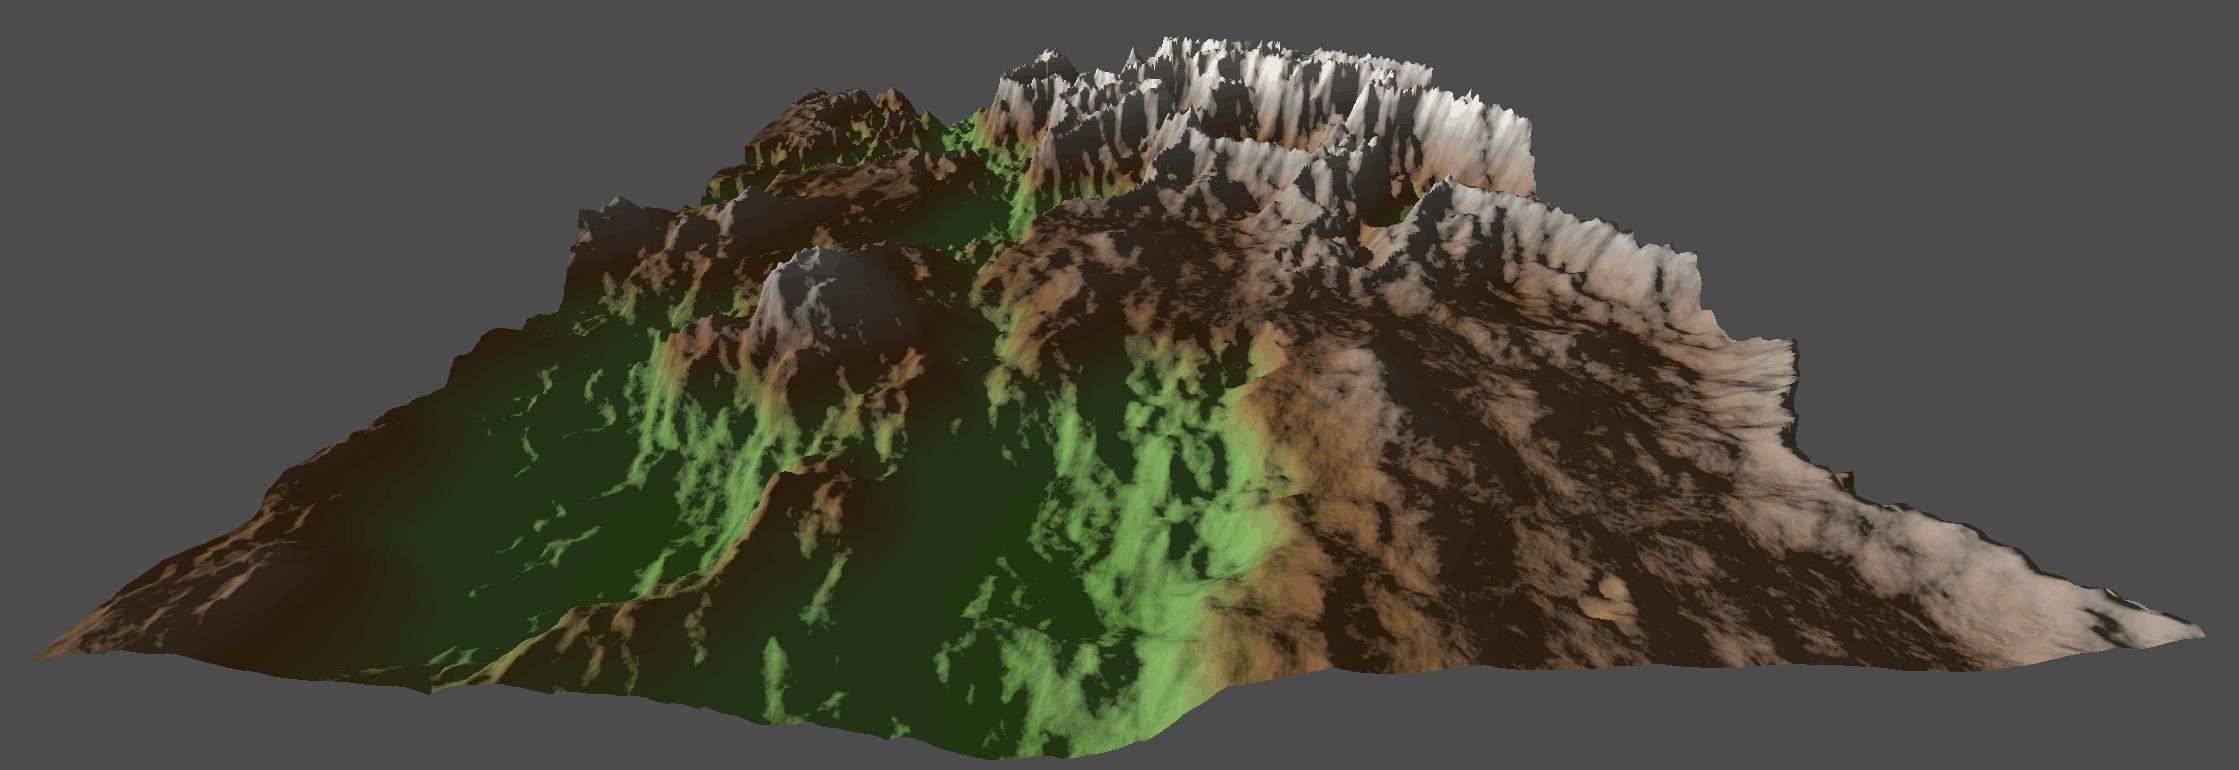
\includegraphics[width=1\textwidth]{obrazky-figures/terrain_showcase.png}
    \caption[Visualization of Expected Terrain]{Visualization of the expected terrain surface. Containing mountain ranges, valleys, and plateaus.}
    \label{fig:terrain_profile}
\end{figure}

The parameters for the surface generation step are primarily the configurations of the noise functions used, the squishing constant, and the targeted terrain height range to which the final value needs to be scaled to obtain the height map.

\subsection{Generation of Underground Caves}

A possible approach to generating underground caves is to use 3D procedural noise. Noise values can be compared against a~defined threshold. If the noise exceeds the threshold, this spot represents a~cavern space filled with air. If it is smaller, then it represents the solid rock walls.

The underground generator also needs to fill the caverns with decorations, as the other generators only work on the surface. Realistic decorations for underground spaces include water, stalactites, and stalagmites. Their placement can be achieved easily. The lowest sections of the caves can be filled with water up to a~defined height, and small waterfalls can be randomly placed on their surface, rising until they reach the cave roofs. Lastly, stalactites and stalagmites could be randomly placed on the ground and roofs of caves.

The parameters of this generator are the configuration values for the 3D noise, the noise threshold, the water level, and the probabilities of placing waterfalls, stalactites, and stalagmites. The expected results of the cave generator are shown as part of Fig.~\ref{fig:final_underground_surface_tunnels}.

\subsection{Generation of Connecting Tunnels}\label{connecting_tunnels_design}

The necessary connections between the underground caves and the surface, as well as between the caves themselves, can be achieved by carving tunnels into the solid ground. Such tunnels could be realized as segments between suitably positioned nodes, obtained by rough sampling of the 3D cave noise. A node would be placed at a~given position if the sampled value exceeds a~defined threshold. As some nodes need to be placed on the surface, the cave noise must be sampled in a~slightly taller area. Each obtained node can then be connected to its closest neighbor (surface nodes connect to underground nodes), thus forming a~network of segments that can be used to carve connecting tunnels.

The tunnel generator parameters include the same 3D noise configuration values as used in the cave generator, along with the node threshold and sampling frequency. The complete underground generation process, with connection tunnels, is shown in Fig.~\ref{fig:final_underground_surface_tunnels}.

\section{Generator of Water Systems}\label{water_systems_generation}
The goal of the water systems generator is to assemble a~water network made of lakes and rivers on the terrain surface. These must be realistically placed in the environment and should reflect the terrain's properties. This generator also needs to estimate water availability in the environment for the subsequent generation steps that handle the generation of biomes and the placement of decoration features.

\begin{figure}[t]
    \centering
    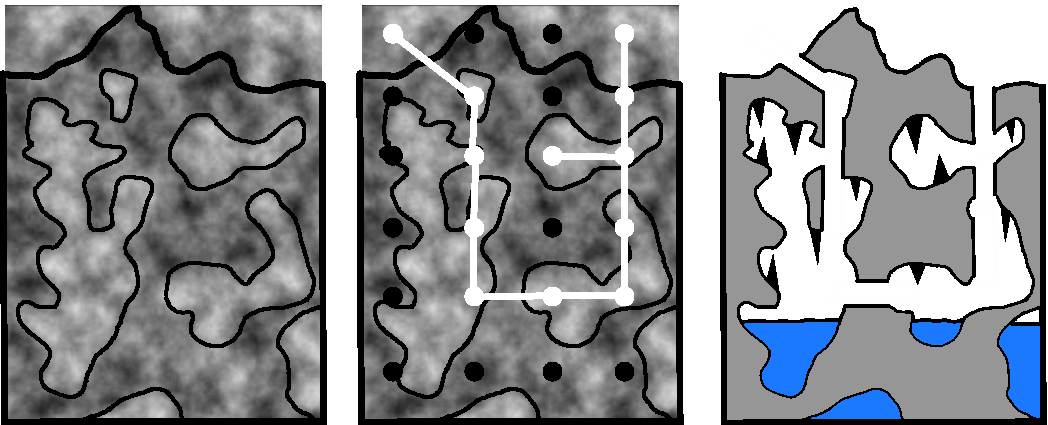
\includegraphics[width=0.75\textwidth]{obrazky-figures/underground_tunnels.pdf}
    \caption[Underground Generation Visualization]{Visualization of the underground generation process on 2D slices. From left to right, 2D noise and thresholded caves, rough node sampling and creation of the network, and the final generated underground with decorations and connecting tunnels.}
    \label{fig:final_underground_surface_tunnels}
\end{figure}

\subsection{Extraction of Lakes}
The terrain height map generated in the previous step is quite rough and bumpy, mostly due to the use of multi-octave noise. This forms many depressions in the terrain, which could be filled with water to form lakes. A suitable method for extracting depressions from a~terrain height map is the Priority-Flood algorithm discussed in Section~\ref{priority_flood}. Thus, this algorithm can be run on the available height map data, and the found depressions can be filled with water and marked as lakes. This process is visualized in Fig.~\ref{fig:lake_extraction}. The only parameters are the depth and size constraints of the depressions.

\begin{figure}[b]
    \centering
    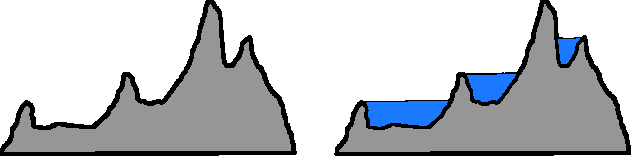
\includegraphics[width=0.65\textwidth]{obrazky-figures/lake_extraction.pdf}
    \caption[Lake Extraction Visualization]{Simple 2D visualization of the lake extraction process. Bumpy terrain with depressions on the left, and terrain with depressions filled by water on the right.}
    \label{fig:lake_extraction}
\end{figure}

\subsection{Generation of Rivers}
The rivers should follow the terrain properties, flowing downhill and draining into the generated lakes. Generally, rivers flow downhill along the fastest and steepest path, which should be the main property of the generator. However, if rivers originate at their sources, the sources must be located first. It is better to generate them in the opposite direction, as the lakes can be extracted fairly easily from the height map. This way, the river's path starts at the edge of a~lake and can be generated based on the height map's gradients. As gradients at specific positions on the height map indicate the direction of the steepest incline, they can be used to guide the rivers on their uphill climb (as shown in Fig.~\ref{fig:gradient_rivers}), thus simulating the property mentioned above in the opposite direction. 

The generator would randomly select a~set of river endpoints around the lake rim. From each of these points, a~river would be generated by the accumulation of nodes along its path, influenced by the height map's gradients. Generation of a~river would stop if it gets too long, if it reaches a~flat surface, or if it starts descending. The width of the river could then be determined for its nodes, based on their distance from the river source.

The parameters of this method include the maximum river length, width calculation parameters, and the distance between two neighboring river entry points on the lake rim.

\begin{figure}[b]
    \centering
    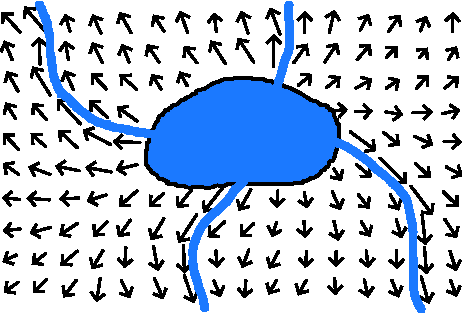
\includegraphics[width=0.4\textwidth]{obrazky-figures/gradient_rivers.pdf}
    \caption[Gradient River Generation]{Visualization of the use of height map gradients for river path guiding.}
    \label{fig:gradient_rivers}
\end{figure}

\subsection{Estimation of Water Availability}\label{water_availability_calculation}
The last step in generating water systems is the estimation of water availability based on the generated lakes and rivers. The effect of these features should be strong close to them and linearly fade with distance. Thus, this task can be solved by applying the effect in circular areas with linear falloff around the lake rims and river nodes. The influence attributed to a~specific position in the environment, from a~certain node or rim point can be calculated with Eq.~\ref{eq:influence_at_distance}, where $base$ is the maximum influence value that can be attributed, $d_{max}$ is the maximum distance at which a~node or rim point can influence the environment, and $dist\left(x, y, node\right)$ is the distance between the position in question and a~node or rim point.

\begin{equation}\label{eq:influence_at_distance}
    \text{inf}\left(x,y\right) = \frac{\text{base} \cdot \left(d_{max} - \text{dist}(x,y, node)\right)}{d_{max}}
\end{equation}

\section{Generator of Biomes with Feature Placement}\label{biomes_features_design}
The goal of this generator is to realistically paint the terrain surface with biome colors and densely populate it with vegetation, decorations, and other features such as snow. Rather than generating a~large set of biomes with varying styles, as in games such as Minecraft, this generator targets natural landscapes and focuses on vegetation.

The generator uses three main position-related attributes, along with biome feature tables and attribute thresholds, to classify environments into biomes and place features. These attributes are terrain height, water availability, and environmental age. When an area is classified into a~specific biome based on attribute thresholds, its ground is colored according to its assigned biome, and the biome feature tables are used to obtain concrete values for the placement probabilities of all vegetation types and some decorations. Then the area is processed on positions of a~2D grid, placing vegetation and decorations based on their likelihoods.

The generator expects models in four main categories -- trees and bushes, land vegetation, water vegetation, and decorations. Tree models must be categorized by their type, size, and health.

\subsection{Effect of Terrain Height}
The elevation of the terrain is the main factor in determining the color of the ground and the placement of deciduous or coniferous trees. Biomes are classified into three main biome types, which are the following:

\begin{itemize}
    \item Lowlands -- very small terrain height, featuring green ground and only deciduous trees.
    \item Highlands -- medium terrain height, featuring green ground and a~mix of deciduous and coniferous trees.
    \item Mountains -- high terrain height, featuring brown ground and only coniferous trees. Snow can occur here.
\end{itemize}

\subsection{Effect of Water Availability}
Water availability affects the overall amount of vegetation that can spawn in an area and determines the health of trees\footnote{Health of trees can be visualized with tree models of different amounts of leaves. Healthier trees should have more leaves, whereas dead trees should have only dry branches.}, which can be either healthy, weak, or dead. It also further influences the ground color. The effect can be seen in Fig.~\ref{fig:water_availability_effect}, and it classifies each main biome into four sub-biomes, which are the following:

\begin{figure}[t]
    \centering
    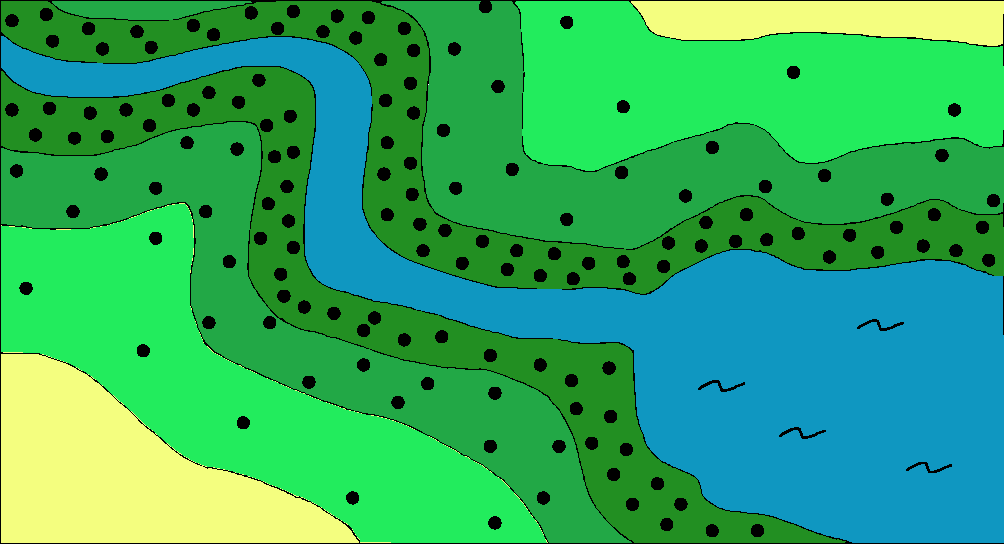
\includegraphics[width=0.5\textwidth]{obrazky-figures/water_effect.pdf}
    \caption[Water Effect on Vegetation Distribution]{Visualization of water availability effect on the distribution of vegetation and ground color. Blue denotes water features. Shades of green and yellow visualize the decrease in water availability with the distance from the water. Black dots denote vegetation.}
    \label{fig:water_availability_effect}
\end{figure}

\begin{itemize}
    \item Dry biomes -- lowlands and highlands have ground color representing sand and can only spawn dead trees. Mountains have stone gray as the ground color.
    \item Biomes with little water -- small amount of vegetation, trees are weak, ground colors are muted, appearing dry.
    \item Biomes with a~medium amount of water -- medium amount of vegetation, trees can be either healthy or weak, ground color is normal.
    \item Biomes with a~high amount of water -- dense vegetation, trees are healthy, ground color is saturated.
\end{itemize}



\subsection{Effect of Environmental Age}
The environmental age is an additional attribute based on low-frequency 2D noise. Its goal is to mimic the distribution of various blends of meadows and forests across the landscape. It affects the spawn rates, actual types of vegetation, and the size of trees. Very young areas are meadows and thus contain only grass, plants, and flowers. As age increases, trees begin to appear, first in smaller sizes, alongside bushes. Older areas feature trees of all sizes, and the amount of small vegetation decreases. The oldest areas feature almost only large trees and very little of small vegetation. This is shown in Fig.~\ref{fig:environmental_age_effect}. An example of classification into 8 sub-biomes and their feature likelihoods is shown in Tab.~\ref{tab:environmental_age_effects}.

\begin{figure}[tb]
    \centering
    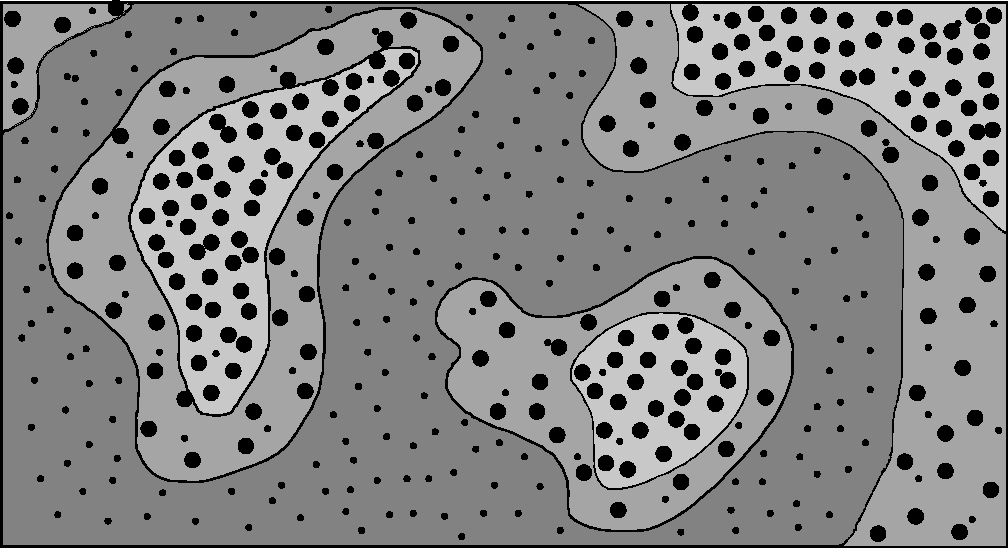
\includegraphics[width=0.5\textwidth]{obrazky-figures/age_noise.pdf}
    \caption[Age Effect on Vegetation Distribution]{Visualization of the effect of environmental age on the distribution of vegetation. Darker gray visualizes younger areas, lighter older areas. Small dots denote small vegetation such as grass and plants. Large dots denote trees.}
    \label{fig:environmental_age_effect}
\end{figure}

\subsection{Placement of Fallen Trunks}
Trunks are placed based on the effects described above, as forests should feature more of them compared to meadows. However, rocks are distributed randomly with equal probability in the environment.

\subsection{Placement of Snow}
The snow placement positions are determined with low-frequency 2D procedural noise. A~spot should be covered with snow if it is located in a~mountainous area and the snow noise exceeds a~configurable threshold.

\subsection{Placement of Water Vegetation}
Water vegetation is placed independently of the mechanism described. All models are randomly placed in lakes according to configurable spawn rates. Reeds and irises are placed in shallow water. Water lilies are placed in medium-deep waters.

\begin{table}[!h]
    \centering
    \begin{tabular}{l|lllll}
        \textbf{Environment Age} & \textbf{Trees {[}S,M,L \%{]}} & \textbf{Bushes} & \textbf{Grass \& Plants} & \textbf{Trunks} \\ \hline
        Very young               & none                          & none                  & very high          & none            \\
        Young                    & none                          & none                  & high               & none            \\
        Young-moderate           & small {[}100,0,0{]}           & small                 & high               & small           \\
        Moderate                 & medium {[}70,30,0{]}          & medium                & medium             & medium          \\
        Moderate-old             & medium {[}35,60,5{]}          & medium                & medium             & medium          \\
        Old                      & high {[}20,50,30{]}           & high                  & medium             & high            \\
        Very old                 & high {[}5,40,55{]}            & high                  & low                & very high       \\
        Ancient                  & very high {[}0,10,90{]}       & very high             & very low           & very high       \\
    \end{tabular}
    \caption[Environmental Age Biomes and their Feature Likelihoods]{Environmental age sub-biomes and their possible feature likelihoods.}
    \label{tab:environmental_age_effects}
\end{table}

%%%%%%%%%%%%%%%%%%%%%%%%%%%%%%
% Demo Implementation Details
%%%%%%%%%%%%%%%%%%%%%%%%%%%%%%
\chapter{Generator Implementation in a~Game Demo}\label{implementation}
This chapter covers the implementation of the world generator described in Chapter~\ref{world-gen-design} in a~pseudo-infinite voxel sandbox video game demo with basic gameplay features and a~similar style to games such as Minecraft and Lay~of~the~Land (see Section~\ref{sandbox-voxel-games}). It has the following features:

\begin{itemize}
    \item Fully procedurally generated environments with custom procedural voxel models implemented based on the design described in Chapter~\ref{world-gen-design}.
    \item Custom highly parallelized chunk system for generation, displaying, and unloading of pseudo-infinite worlds via a~dynamic hierarchical system of distributed tasks.
    \item Basic camera movement options, including support for walking on the world surface and collision-free flying.
    \item Basic user-based voxel editing of the whole voxel space.
    \item Simple sun cycle and toggle-able torch-like light source positioned near the camera.
    \item Support for teleportation to specified world positions.
    \item Support for multiple worlds and their saving and loading, including edited voxels.
    \item Support for complex configurable options during creation of new worlds.
    \item Basic UI, including main menu, world creation and configuration, loading, visuals configuration screen, and pause menu.
\end{itemize}

The demo is implemented in the Godot~Engine\footnote{Godot Engine website: \href{https://godotengine.org/}{\texttt{godotengine.org}}} 4.6.2. The language of choice is C\#\footnote{.NET homepage: \href{https://dotnet.microsoft.com/en-us/}{\texttt{dotnet.microsoft.com/en-us}}}. Implementation depends only on built-in functionality and libraries of C\# supplied by the .NET 10 runtime, and libraries and abstractions provided by Godot~Engine. The most important of which is the embedded FastNoiseLite\footnote{FastNoiseLite github repository: \href{https://github.com/Auburn/FastNoiseLite}{\texttt{github.com/Auburn/FastNoiseLite}}} library, which was used to obtain 2D and 3D noise values throughout the world generation system. The project contains a~single third-party engine extension, which is Debug Menu\footnote{Godot Debug Menu extension: \href{https://github.com/godot-extended-libraries/godot-debug-menu}{\texttt{github.com/godot-extended-libraries/godot-debug-menu}}} for in-game performance tracking.

The Godot Engine is used as a~renderer, a~physics engine for player movement and collisions, an I/O abstraction layer, and for creating the user interface. All other aspects of the demo, including voxel management, a~chunk system for pseudo-infinite generation and unloading, and support for generating and applying geometry at different levels of detail, were implemented as part of this thesis and are discussed in the following sections.

\section{Architecture of Demo Implementation}

The simplified architecture pipeline of the demo is visualized in Fig.~\ref{fig:basic_architecture_overview}. The main goal is to procedurally generate the world and display it on the screen, while also allowing other features such as voxel editing, user interfaces, and more.

The first step is to procedurally generate the world in a~simplified internal representation. Then it is necessary to voxelize it into internal voxel structures. And finally, it needs to be displayed on the screen. This demo implements this via the general GPU pipeline that utilizes surface geometry. However, this geometry must first be extracted from the voxel space before it is displayed using the Godot Engine. The main reasoning behind this proposed architecture is the following:

\begin{figure}[t]
    \centering
    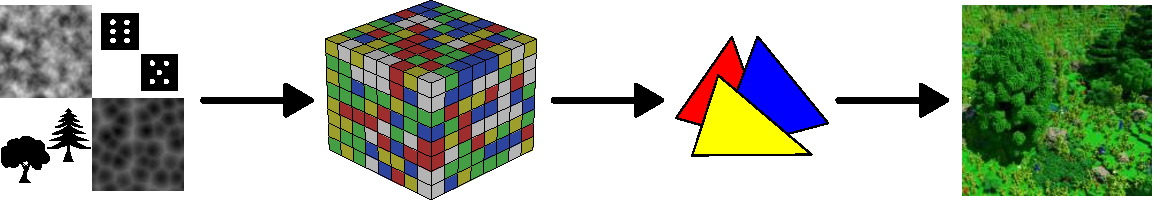
\includegraphics[width=1.0\textwidth]{obrazky-figures/basic_arch_overview_opti.pdf}
    \caption[Basic Implementation Architecture]{Simplified architecture of the demo. From left to right, procedural world generation, voxelization, geometry extraction, and finally, visualization.}
    \label{fig:basic_architecture_overview}
\end{figure}

\begin{itemize}
    \item It allows a~clean separation of the problem into sub-problems and a~hierarchical structure, which is suitable for parallelization and for encapsulating internal details.
    \item The internal voxel representation enables complete editing of the world environment. It also simplifies the implementation of caves and the creation of some models. These generators can directly paint into the voxel structure, treating it as a~3D canvas.
    \item The general GPU pipeline, oriented around the visualization of surface geometry, is a~standard supported by all GPU manufacturers. Simple scenes with short render distances can be rendered even on GPUs with limited resources.
\end{itemize}

\subsection{World Subdivision with a~System of Chunks}
As stated several times in this thesis, this project aims to support large pseudo-infinite voxel environments. This leads to the use of chunk systems as discussed in Section~\ref{chunk_systems}. The world space is divided into small sections that are generated and unloaded based on the camera's current position and used throughout the entire demo pipeline.

This demo uses two different sizes of world sections (chunks). The first consists of large regions used to represent mostly 2D information generated by the world generation process. The second consists of columns of symmetrical 3D chunks. These are used to store 3D voxel-space information and the generated geometry. 

The world space is thus divided into a~multi-layer 2D grid of World Regions and Chunk Columns, of which only a~small number around the camera are active at any given time. This is shown in Fig.~\ref{fig:chunk_system_camera}. The following sections discuss their details, generation, and unloading.

\begin{figure}[t]
    \centering
    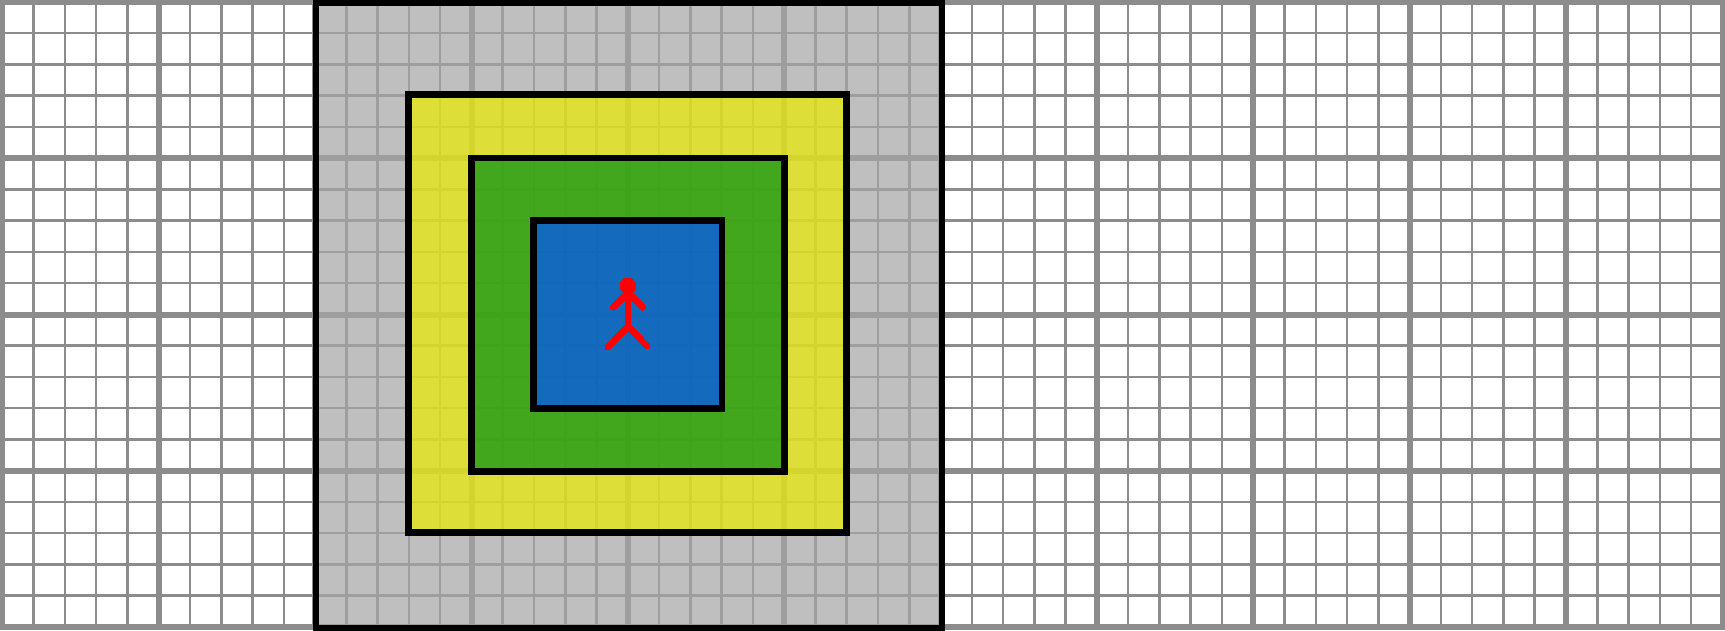
\includegraphics[width=1.0\textwidth]{obrazky-figures/chunk_columns_camera.pdf}
    \caption[Chunk System with Camera]{Visualization of the chunk system, including active sections around the camera. Large gray background cells denote World Regions, smaller cells Chunk Columns. The camera is visualized by the red character. The blue area denotes currently displayed Chunk Columns, the green area is for geometrized Chunk Columns, the yellow area means voxelized Chunk Columns, and the gray area is for active World Regions.}
    \label{fig:chunk_system_camera}
\end{figure}

\subsection{Detailed Demo Architecture}

The detailed architecture of the demo is shown in Fig.~\ref{fig:architecture_full}. The demo is controlled by the Game Manager, based on user interaction with the user interface, player camera movement, and user-supplied voxel editing operations. The demo can find itself in one of the states shown in the simplified FSM in Fig.~\ref{fig:simple-demo-fsm}. Apart from the less important user interface sub-states, there are two main states, which are the following:

\begin{itemize}
    \item World Inactive -- no world is currently active. The chunk system is disabled. The main menu or some of its sub-menus are shown.
    \item World Active -- world is active, or it is being prepared. The chunk system is enabled. Voxel editing is possible. Can be in-game or in the pause menu.
\end{itemize}

\begin{figure}[t]
    \centering
    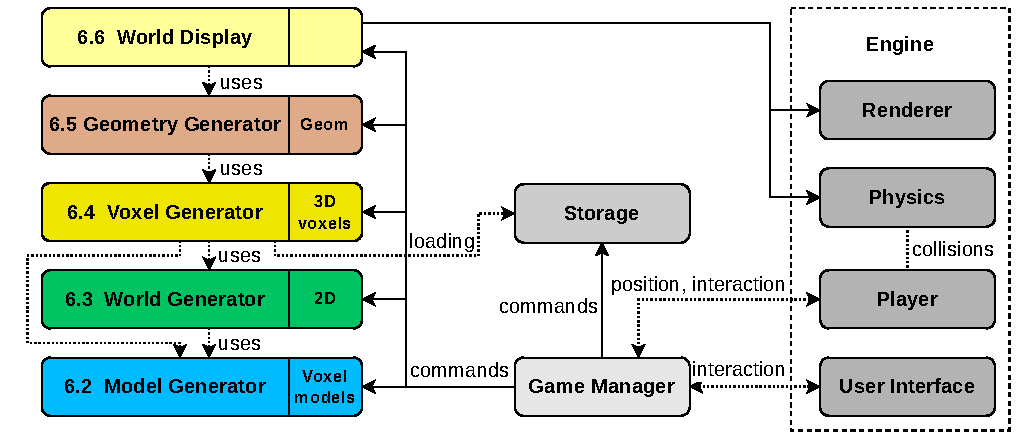
\includegraphics[width=1.0\textwidth]{obrazky-figures/architecture.pdf}
    \caption[Implementation Architecture]{Detailed architecture of the demo. The left side denotes the hierarchical chunk system and Model Generator. The right side denotes Godot Engine-related components. The numbering of components on the left corresponds to their sections in the following text. The same applies to the color coding in the following diagrams.}
    \label{fig:architecture_full}
\end{figure}

The state World Active is of importance and is thoroughly described in the following sections. Alg.~\ref{alg:world_active_algorithm} summarizes the most important events during this state.

\begin{algorithm}
\caption{Game Manager control of the demo when a~world is active}\label{alg:world_active_algorithm}
\begin{algorithmic}[1]
\State Create new world or load configuration of an existing one from \textit{Storage}
\State Initialize all components of the system
\State Start \textit{Model Generator}, \textbf{wait} for it to finish
\While{\textit{World} is \textsc{active}}
\State Manage the chunk system based on the current \textit{Player} position
\State Process voxel editing operations, save them to \textit{Storage}
\State Process user interface events
\EndWhile

\end{algorithmic}
\end{algorithm}

\subsubsection{Hierarchical Chunk System}

The most important part of the demo implementation is the hierarchical chunk system, which is controlled by the Game Manager, as shown in Fig.~\ref{fig:architecture_full}. When the game is active, the Game Manager dynamically schedules distributed tasks and triggers unloads across all layers of the hierarchical system based on the camera's movement.

Each layer processes its own tasks with up to its configured number of threads. The diagram also shows the dependencies of each layer. The higher layers depend on the layers below them, and tasks that require work still in progress in the lower layers are postponed until their dependencies are fulfilled. In the meantime, other tasks can be processed in the layer. For example, the Geometry Generator will receive a~task to generate a~specific column, and it will be postponed until the Voxel Generator finishes voxelization of that column, potentially waiting for World Region generation as well.

\subsubsection{Introduction to Chunk System Layers}

As already mentioned, the layers are discussed in detail in their own sections. Here follows only a~very simple summary of each layer:

\begin{itemize}
    \item Model Generator -- generates voxel models for further use in the hierarchical system. Runs at the start of the world loading process. Other layers start after it is finished.
    \item World Generator -- pre-generates the world in large World Regions. Prepares the height map, some parts of the caves, water map, biomes, and feature placements.
    \item Voxel Generator -- voxelizes sections of the World Regions into columns of symmetrical chunks, producing the voxel representation. Applies edited voxels from Storage.
    \item Geometry Generator -- extracts chunk column geometry from voxel representation.
    \item World Display -- communicates with the engine to display chunk column geometry.
\end{itemize}

\begin{figure}[tb]
    \centering
    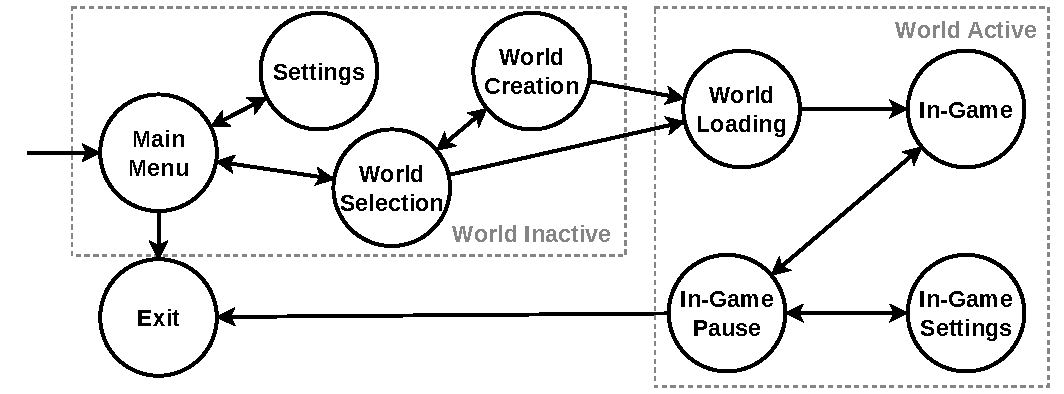
\includegraphics[width=0.85\textwidth]{obrazky-figures/demo_fsm.pdf}
    \caption[Simple Demo FSM]{Simplified demo FSM, with two main states -- world active or inactive.}
    \label{fig:simple-demo-fsm}
\end{figure}

\subsubsection{Scheduling of the Distributed Tasks}

The Game Manager stores information on which regions and columns are currently active across all layers of the hierarchical system. When the camera moves, its new position is mapped to the chunk grid, and symmetrical rectangular areas are mapped around it. Each of these rectangular areas represents the space that needs to be active for one of the layers of the hierarchical system. This way, the Game Manager determines which chunks must be active in each layer. This information is then compared with the previously stored configuration of the chunks. New chunks that were not present in the previous configuration are marked as active, and their generation or display tasks are scheduled in their layers.

The unloading of inactive chunks is done with a~similar mapping but uses larger rectangular areas. Chunks that fall out are marked as inactive and are unloaded from their respective layers. This way, there is a~buffer area, reducing the number of chunks that are repeatedly loaded and discarded, thereby saving computation time.

The process of mapping the camera to the chunk grid and the set of symmetrical rectangular areas around it that denote chunks and regions currently active is shown in Fig.~\ref{fig:chunk_system_camera}.

\subsubsection{Godot Engine Integration}

The right side of the architecture diagram in Fig.~\ref{fig:architecture_full} shows the integration in the Godot Engine. User interfaces and Player components are Godot Engine scenes that communicate with the Game Manager's main script, which is attached to the root scene of the Godot project. The World Display service then communicates with the engine to configure currently rendered chunk geometry and collision layers for the physics subsystem based on the tasks it receives from the Game Manager. More details about this process are discussed in Section~\ref{world_display_layer}.

\section{Model Generation Layer}

The Model Generator encapsulates the entire voxel model generation process. It runs only once per world during its startup. The rest of the hierarchical generation system waits for it to finish and starts afterward. It is not possible to run the generator only once at application startup, because voxel model generators use a~seed value that can differ between worlds.

The generator is initialized with a~list of voxel model definitions, a~world seed, and the number of threads it can use. Initialization is handled by the Game Manager, which also starts the generation process and collects the generated models once its completion is signaled. The generator supports vegetation models of trees, bushes, grass, plants, flowering bushes, reeds, and water lilies, as well as trunk, rock, and stalactite decoration models.

The list of model definitions contains multiple definitions for each model type to increase the variety of vegetation and decorations. Tree models are also categorized into three groups based on type (deciduous or coniferous), size (small, medium, or large), and health (dead, weak, or healthy). However, if the same model definition were run with the same world seed, all resulting models would be identical. Thus, to enable both variation and determinism, the model generator assigns a~specific seed value to each model definition as $seed_i = seed_{world} + i$, where $seed_i$ is the seed for model definition at index $i$ in the ordered definition list.

The actual generators of the supported models are implemented exactly as specified in their design in Section~\ref{voxel_model_generation_design}. However, some implementation details, especially regarding the voxelization of these models, are discussed in the following sections.

\subsection{Voxel Model Structures}

The voxel model generators use a~rectangular cuboid 3D voxel space mapped to 1D arrays, where each position stores a~voxel cube of the same size as the smallest voxel in the voxel storage, which is $1/16$~m. This is done because vegetation and decorations require the highest level of detail possible in the system.

After a~model is generated, it is collapsed into an array of Voxel Items without empty (air) voxels, where each Voxel Item stores a~3D position and its voxel type. This is done to optimize the later application of the voxel models to the voxel space of Voxel Storage, as the voxel models are highly sparse and most of the 3D positions correspond to empty (air) voxels, which are skipped during application.

Some of the methods do not use the described voxel model structure. Instead, due to their simplicity, they generate lists of Voxel Items directly and convert them to arrays.

\subsection{Generation and Voxelization of Simple Models}

Generators for models of small plants, such as grass, plants, water plants, and flowering bushes, are implemented almost exactly as described in their designs. All of these generators leverage basic geometric properties of these plants, and their simplicity allows them to directly produce Voxel Items that are assembled into lists and then exported to arrays. The majority of the blooms are predefined sets of voxels that are placed at the ends of procedurally generated stems.

When it comes to the generation of decorations, stalactites are very similar to models of small plants. Their generator again uses geometric properties to directly assemble lists of voxels. On the other hand, the generators for rocks and trunks use the voxel model structures. Rocks are generated by voxelizing 3D procedural noise values that cross the threshold of an outward-growing spherical gradient. The generator of fallen trunks internally uses the tree generator, which is discussed in the next section. The tree is generated without leaves, and the generation process is run for only a~handful of iterations. The voxel model is transformed to a~lying position, and then rotated to one of four defined positions ($\pm X, \pm Z$). Only four positions were chosen to simplify the implementation.

\subsection{Generation and Voxelization of Trees and Bushes}

The generator of trees and bushes uses the Space Colonization algorithm and the discussed solutions for attraction point generation, as described in Section~\ref{generation_trees_bushes}. However, their generator cannot directly paint into voxel structures. After the Space Colonization algorithm is finished, it is necessary to first calculate the segment radii of the resulting branching structure. The segments are then classified into branches and leaf segments.

All branches (including leaf segments) are made of sets of nodes. These nodes are used as control points of the Bézier curves, and the curve path along them is evaluated by de~Casteljau's algorithm (see Section~\ref{bezier_de_casteljau_algo}). Along this path are voxelized spheres with the same radius as the branch, which fill the model's voxel space with wood voxels. Segments with leaves also generate leaf patches around all nodes of the branch, randomly with a~defined dispersion. These leaf patches are voxelized into spheres, this time with leaf voxel types. Non-air voxels are then extracted and returned in an array of Voxel Items.

\section{World Generation Layer}

The World Generation layer procedurally generates information about the world environment by creating large World Regions that store mostly 2D data, such as terrain height maps, water maps, biome maps, and voxel model placements. A detailed section of the demo architecture diagram is shown in Fig.~\ref{fig:world_generator_in_arch}. The layer is managed by the World Generator Service, which receives generation tasks and unload commands from the Game Manager. It controls the active World Regions and uses World Generator and other components to generate them. Tasks scheduled by the Game Manager specify which World Regions should be generated and made available, and at which generation stage. These tasks are then processed in parallel.

\begin{figure}[tb]
    \centering
    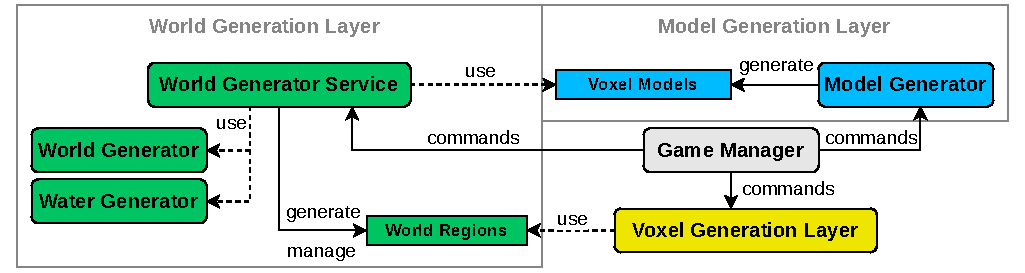
\includegraphics[width=1.0\textwidth]{obrazky-figures/world_generator_service.pdf}
    \caption[World Generation Layer]{Detailed World Generation layer architecture diagram.}
    \label{fig:world_generator_in_arch}
\end{figure}

The procedural generation of the world environment closely follows the world generator design discussed in Chapter~\ref{world-gen-design}. However, significant differences and implementation details are described in the following sections. Firstly, the generation process of a~region is divided into two stages, which are outlined in Fig.~\ref{fig:world_region_generation_stages}. Secondly, the generation process of underground caves mostly happens in the Voxel Generation Layer.

\begin{figure}[b]
    \centering
    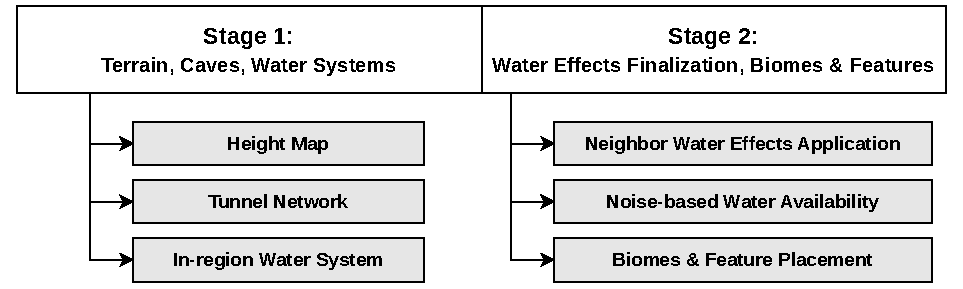
\includegraphics[width=0.95\textwidth]{obrazky-figures/world_region_stages.pdf}
    \caption[World Region Stages]{Visualization of the two stages of World Region generation.}
    \label{fig:world_region_generation_stages}
\end{figure}

\subsection{Negative Effects of Environment Segmentation}\label{world_gen_negative_segmentation_effects}

Environment segmentation and its generation in sections are necessary to support pseudo-infinite worlds. However, it also creates implementation issues. Especially when it comes to the generation of water systems and their effects on water availability. Potentially causing issues with visible seams and limited lake and river generation.

The water system generator proposed in Chapter~\ref{world-gen-design} can be scaled down and implemented to run within regions of the world without issues. However, this will mean that rivers and lakes cannot cross regional boundaries and, depending on the size of the regions, can be significantly limited in length and size. This can be at least partially mitigated by increasing the size of the regions, so that the negative effect is less noticeable. As a~result, World Regions are truly large, covering an area of $256$ by $256$ meters.

Furthermore, a~bigger problem arises with the effects of lakes and rivers on water availability. If this effect is not shared across region boundaries, there will be a~visible difference in the ground voxel color and in the amounts and types of vegetation right at the region boundaries. This is due to differences in biome classifications, as water availability values can change sharply at boundaries.

The most straightforward solution to this problem is to share the effects on water availability across regional boundaries. However, this considerably complicates the generation due to inter-regional dependencies. Thus, the implementation divides the process into two stages, as shown in Fig.~\ref{fig:world_region_generation_stages}. Generation at stage one has no dependencies. But to generate a~region at stage two, it is necessary that all 8 neighbors of the region have finished stage one, as is shown in Fig.~\ref{fig:stage_one_stage_two_regions}. This is also reflected in the Game Manager and chunk system management, which needs to track two stages of World Region generation.

\begin{figure}[t]
    \centering
    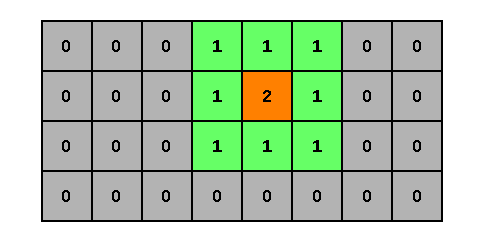
\includegraphics[width=0.6\textwidth]{obrazky-figures/stage_one_stage_two_region.pdf}
    \caption[Region Neighbor Stages]{Necessary neighbor region stages to generate a~World Region at stage 2.}
    \label{fig:stage_one_stage_two_regions}
\end{figure}

\subsection{Generation of Underground Caves}

Another difference from the world generator proposed in Chapter~\ref{world-gen-design} is the generation of underground cave space. Because the World Regions cover large sections of the environment, it is not possible to pre-generate cave spaces, as they would require a~memory-heavy voxel representation. However, the formation of underground caves involves the development of tunnel networks, which are necessary to connect the surface to the caves and the caves to each other. The generation of such a~network would be complicated during the voxelization process in the Voxel Generation layer, where the environment is processed on very small columns, thereby considerably limiting the length of tunnel connections. Thus, the cave generation process is divided into two parts. The actual cave spaces are generated in the Voxel Generation layer by immediate voxelization of 3D procedural noise. And the network of tunnels is generated and pre-voxelized in the World Generation layer, utilizing the large space covered by World Regions to assemble believable connecting tunnels.

\subsection{World Region Data Structure}

The World Generation layer stores its information in a~dynamic grid of World Regions, represented by a~concurrent dictionary. Each World Region stores the data listed in Fig.~\ref{fig:world_region_structure}. Most of the information is stored in a~2D grid of terrain cells, where each cell represents a~surface area of $1/4$ by $1/4$ meters. The map of disabled positions stores terrain surface cells in the vicinity of ground tunnel entrances. The spilled water effects component stores the water effects on water availability, which spill from this region into its 8 neighboring regions.

The height, ground color, and water availability maps are represented as 2D arrays. As snow and water maps are highly sparse, they are represented as dictionaries. Feature placements store positions of vegetation and decorations on the terrain surface. Pre-voxelized tunnels contain 3D voxel positions that must be carved during cave generation in the Voxel Generation layer. Both feature placements and pre-voxelized tunnels are stored in a~per-column structure for fast access in Voxel Generator.

\subsection{Generation of Terrain Height Map}

The terrain height map generation utilizes the designed noise transformations discussed in Section~\ref{terrain_surface_height_map}. The region is traversed in both $X$~and $Z$~axes, and for each terrain cell (which is $1/4$ by $1/4$ meters), a~value in the range $\left(0,1\right)$ is obtained and then scaled to a~configurable range of the resulting terrain height.

\subsection{Generation of Tunnels Connecting Caves and the Surface}

Tunnels connecting the surface with underground caves and the caves with each other are generated based on the proposed design discussed in Section~\ref{connecting_tunnels_design}. The thresholds for tunnel nodes are split into surface and underground ones, allowing detailed configuration during world creation.

After the segments are generated, they are also pre-voxelized, and the resulting voxels are stored as carving operations independently for each Chunk Column of the region.

Voxelization is performed by spheres of defined radius moving along the segment lines of the tunnel network. The process also checks for surface intersections, marking surface cells as disabled for vegetation and decoration placement so they do not float in mid-air. When obtaining the surface nodes, nodes too close to water features are also skipped to minimize interruptions.

\begin{figure}[t]
    \centering
    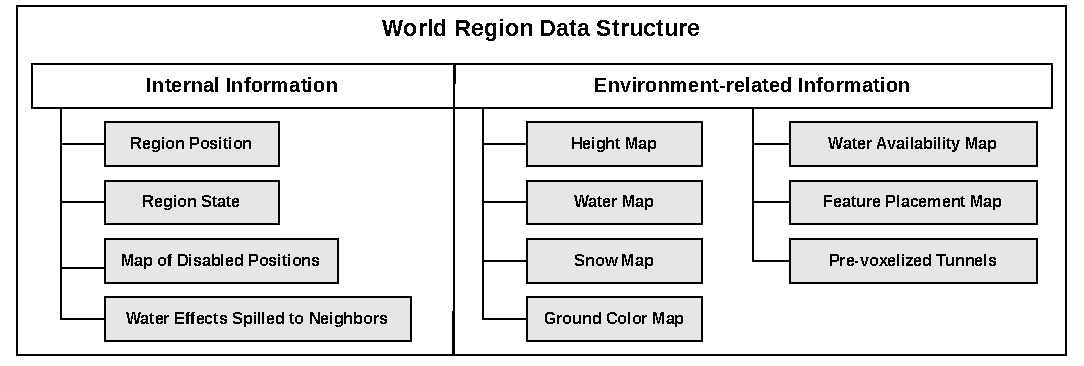
\includegraphics[width=1.0\textwidth]{obrazky-figures/world_region_structure.pdf}
    \caption[World Region Structure]{World Region data structure with the most important stored elements.}
    \label{fig:world_region_structure}
\end{figure}

\subsection{Generation of Water Systems}

The generation of lakes and rivers is again implemented closely to the design discussed in Section~\ref{water_systems_generation}. However, there are some important differences, due to the negative effects of world segmentation, as discussed in Section~\ref{world_gen_negative_segmentation_effects}. For example, the Priority-Flood algorithm proceeds inward, so if a~terrain depression stretches across a~region boundary, a~lake cannot be placed there. Instead of only scaling down the water system generation to run within regions, the surface area is also explicitly filled with water up to a~defined height. This allows the formation of lakes and other water surfaces that can cross regional boundaries. Rivers are generated from their rim as well.

The first step in river generation is the pre-computation of gradient fields at two resolutions, which are $1$~and $4$-meter cells. When a~rim point is selected for river generation, the algorithm follows the path of the steepest incline in the height map, as indicated by the gradient field. At each point along the path (spaced $1$~m apart), the gradient field is first sampled at $ 1$-meter resolution. If a~flat area is detected, the gradient field is resampled at 4-meter resolution. If the terrain still appears flat, the algorithm can continue for a~few more steps. It stops when a~river of maximum length is formed, the terrain remains flat for too long, or in edge cases such as loops or downhill sections. In this manner, a~rough set of nodes along the river trajectory is generated, which can serve as control points for a~Bézier curve to produce a~smooth river path. This smooth path is then traversed, its varying width is calculated based on the distance from its source, and it is applied to the water map by adding circles of water that are deeper in the center and shallower at the edges.

The water map indicates how many terrain voxels ($1/4$~m in each axis) of water should be placed above the terrain for positive values (lakes) or carved into the terrain for negative values (rivers).


\subsection{Calculation and Application of Water Availability Effects}

The effects of lakes and rivers on water availability accumulate through a~three-step process. Firstly, each region, during its first stage of generation, calculates water effects exactly as specified in Section~\ref{water_availability_calculation}. The effects that spill outside the region are stored for each of the region's 8 neighbors. In the second generation stage of the World Region, the effects leaking from its neighbors are applied to it. Then, all positions within the region are further influenced by values from a~2D procedural noise field, simulating a~groundwater-like effect. This is done to smooth out water availability in the region and reduce the chance that an area will be completely arid.

\subsection{Biomes and Feature Placement}

At the end of the region generation process, biomes are generated, and vegetation and decoration features are placed in a~two-step process exactly as discussed in Section~\ref{biomes_features_design}.

The biomes are classified on a~per-terrain cell basis, with surface colors saved to the World Region's ground color map. This part of the biome classification is influenced by terrain height and water availability. An excerpt of this process is outlined in Alg.~\ref{alg:biome_color_class_excerpt}.

\begin{algorithm}
\caption{Excerpt of biome classification for surface coloring}\label{alg:biome_color_class_excerpt}
\begin{algorithmic}[1]
\For{$x$ in $x_{size}$}
\For{$z$ in $z_{size}$}
\If{height$\left(x,z\right)$ < lowlands}
\If{water$\left(x,z\right)$ < arid}
\State ground$\left(x, z\right) = color_{sand}$
\EndIf
\If{water$\left(x,z\right)$ < low}
\State ground$\left(x, z\right) = color_{green}$
\EndIf
\State \dots
\EndIf
\EndFor
\EndFor
\end{algorithmic}
\end{algorithm}

The feature placements in a~region are then generated on a~per-voxel cell basis. Each cell is $1/16$ by $1/16$ meters and has a~chance to spawn vegetation and decorations. Whereas water plants are randomly distributed in lakes, other vegetation and decorations are positioned based on water availability, terrain height, and environmental age, which influence their chances throughout the region, exactly as described in the design section.


\section{World Voxelization Layer}\label{voxelization_layer}

The World Voxelization layer voxelizes large World Regions into small vertical Chunk Columns that store 3D voxel information, and together with the Game Manager, it manages the voxel space. It works similarly to other layers of the hierarchical system, processing tasks scheduled by the Game Manager in parallel once their dependencies are fulfilled. Its detailed architecture and important connections to the rest of the demo components are shown in Fig.~\ref{fig:world_voxelization_service}. Internally, the service uses the Voxel Generator to voxelize the Chunk Columns, and it also needs the voxel models to instantiate them into the voxel space. User voxel editing is also handled by the Game Manager.

\begin{figure}[t]
    \centering
    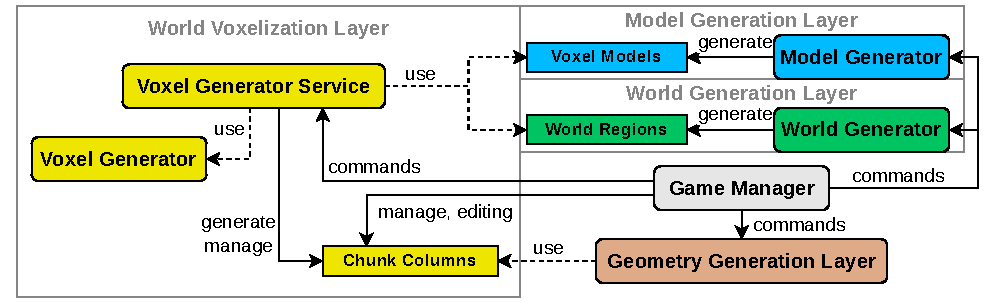
\includegraphics[width=1.0\textwidth]{obrazky-figures/world_voxelization_service.pdf}
    \caption[World Voxelization Layer]{Detailed World Voxelization layer architecture diagram.}
    \label{fig:world_voxelization_service}
\end{figure}


\subsection{Voxel Storage}

The demo uses a~custom Voxel Storage solution. It is a~dynamic dictionary that stores active Chunk Columns of the 2D world grid. Each Chunk Column consists of vertically stacked symmetrical chunks. Each of them represents a~root node of SVO structures (see Section~\ref{svos}). This can be seen in Fig.~\ref{fig:chunk_column_visualization}. Chunk Columns are significantly smaller than World Regions, as each vertically stacked chunk represents $4$ by $4$ by $4$ meters of the world environment.

\begin{figure}[b]
    \centering
    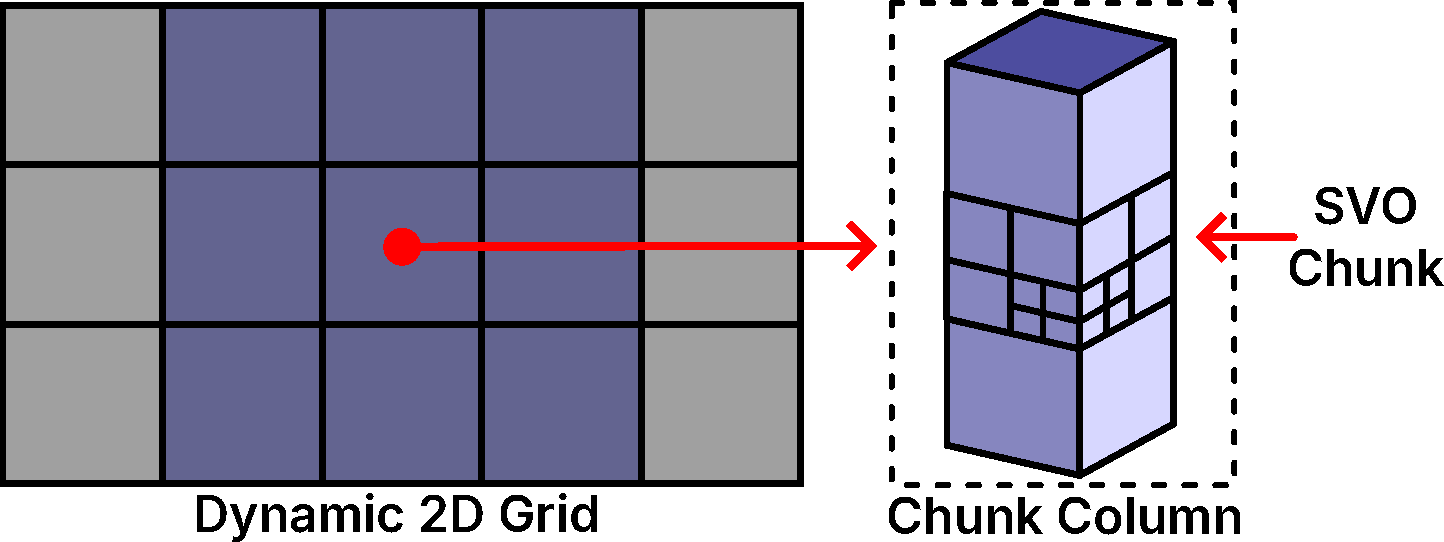
\includegraphics[width=0.6\textwidth]{obrazky-figures/chunk_columns_visualization.pdf}
    \caption[Chunk Columns Visualization]{Visualization of Chunk Columns and their dynamic 2D grid. Gray cells denote inactive segments. Blue cells active ones.}
    \label{fig:chunk_column_visualization}
\end{figure}

The Voxel Storage in this demo is highly detailed, with the smallest voxel cube measuring $1/16$~m in each axis. This large number of voxels is also the main reason why SVOs are used, as they can dramatically reduce the memory requirements. They are also used for efficient variable-sized queries and editing operations in the voxel space.

The voxelization process directly paints into the Voxel Storage at varying levels of detail, and the same happens during user-based world editing. However, this does not yield an optimal representation of the voxel space for SVOs, as many collapsible sections are present. Thus, after voxelization of a~Chunk Column is complete, a~simplification operation is run that traverses the column's SVO chunks and collapses them into an efficient state. During this process, the most prevalent non-air voxel types are also set as the voxel types of the parent SVO nodes, simplifying the implementation of geometry generation at various levels of detail. The same process must also occur after each user-editing operation.

To further optimize the Voxel Storage for geometry extraction, the Chunk Columns form an interconnected network. This is beneficial as the Geometry Generator needs to work with neighboring columns when generating geometry at column boundaries, and quick access via an interconnected network is faster than a~lookup and multiple function calls.

The voxel types in this game demo are solid-colored cubes that can be used to assemble the world's environment. Some voxel types are handled specifically during visualization, such as air voxels, which denote empty space. Others include voxel types denoting submerged plants, which are required to overcome visualization limitations.


\subsection{Voxelization and Model Application Process}

The voxelization of a~single Chunk Column is a~four-step process, including initialization, voxelization of terrain and caves, instancing of features, and application of the snow layer. In the end, stored voxel editing operations are applied, and all chunks of the column are simplified.

\subsubsection{Chunk Column Dependencies}

In order to voxelize a~single column, it is necessary that its region, as well as the regions of its 8 neighboring columns, are generated. This is because, depending on the placement of features, their voxels often leak into neighboring columns. The voxelization process solves this by finding and applying voxels that leak from neighboring columns into the column currently being generated.

Originally, it was planned that this would be implemented the other way around -- voxelization of a~column would paint its leaking voxels to its 8 neighbors. However, issues with its implementation, determinism problems, and missing features after subsequent loading and unloading steps led to the implementation described above.

\subsubsection{Voxelization of Terrain and Caves}

The voxelization of terrain and cave space is performed in a~single iteration. The voxel space of a~Chunk Column is traversed in sub-columns on voxels of terrain size ($1/4$~m in all axes). These sub-columns are traversed vertically from bottom to top.

The cave space is directly voxelized with values from 3D procedural noise, mapped to air or different types of stone voxels based on defined noise thresholds. The lower cave levels are filled with water up to a~specified height, and the locations of waterfalls, stalactites, and stalagmites are chosen randomly. Waterfalls are also directly voxelized as columns of water voxels.

Then, the surface area is voxelized as well. Below the surface are some stone and dirt voxels. On top of it are ground voxels with colors determined by the generated biomes. Water voxels are either placed on the surface for lakes or carved into the surface when voxelizing rivers.

\subsubsection{Application of Voxel Models}

Then, the voxel models are instanced into the Chunk Column by applying all the voxels from these models to its voxel space. First, the voxels of stalactites and stalagmites are applied, with placements generated in the previous step. Then the column applies the voxels from its own features, skipping voxels that leak outside it. Lastly, all feature placements of its 8 neighbor columns are traversed, and the voxels that leak into the current column are applied to it. The voxels are applied only to positions where there is air. Plant voxels placed in water are converted to submerged plant voxels.

\subsubsection{Application of Snow Layer}

The last step is the application of the snow layer. The voxel space is first quickly traversed from top to bottom to find the first chunk that contains non-air voxels. Then, the column is traversed in horizontal cells. If a~cell should be covered by snow, its voxel sub-column is traversed down until the first non-air voxel is found, and a~snow voxel is placed on it.


\section{Geometry Generation Layer}



The Geometry Generation layer extracts cubical surface geometry from the voxel space for display using the general GPU pipeline. Similarly to the rest of the layers of the hierarchical system, it is managed by tasks supplied by the Game Manager, as shown in Fig.~\ref{fig:geometry_generation_service}.

The Geometry Generator Service processes tasks with fulfilled dependencies in parallel. The voxel space is processed in Chunk Columns, and their surface geometry is extracted, forming Chunk Column Geometry structures. The geometry is generated at three levels of detail (LOD), enabling high-quality detail while also improving rendering performance and reducing VRAM usage for chunks farther from the camera. A~simple visualization of the main goal of the Geometry Generation layer is shown in Fig.~\ref{fig:geometry_visualization}.

\begin{figure}[t]
    \centering
    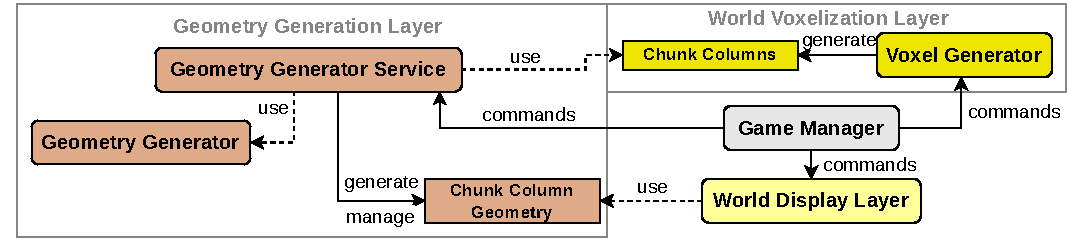
\includegraphics[width=1.0\textwidth]{obrazky-figures/geometry_generation_service.pdf}
    \caption[Geometry Generation Layer]{Detailed Geometry Generation layer architecture diagram.}
    \label{fig:geometry_generation_service}
\end{figure}

\begin{figure}[b]
    \centering
    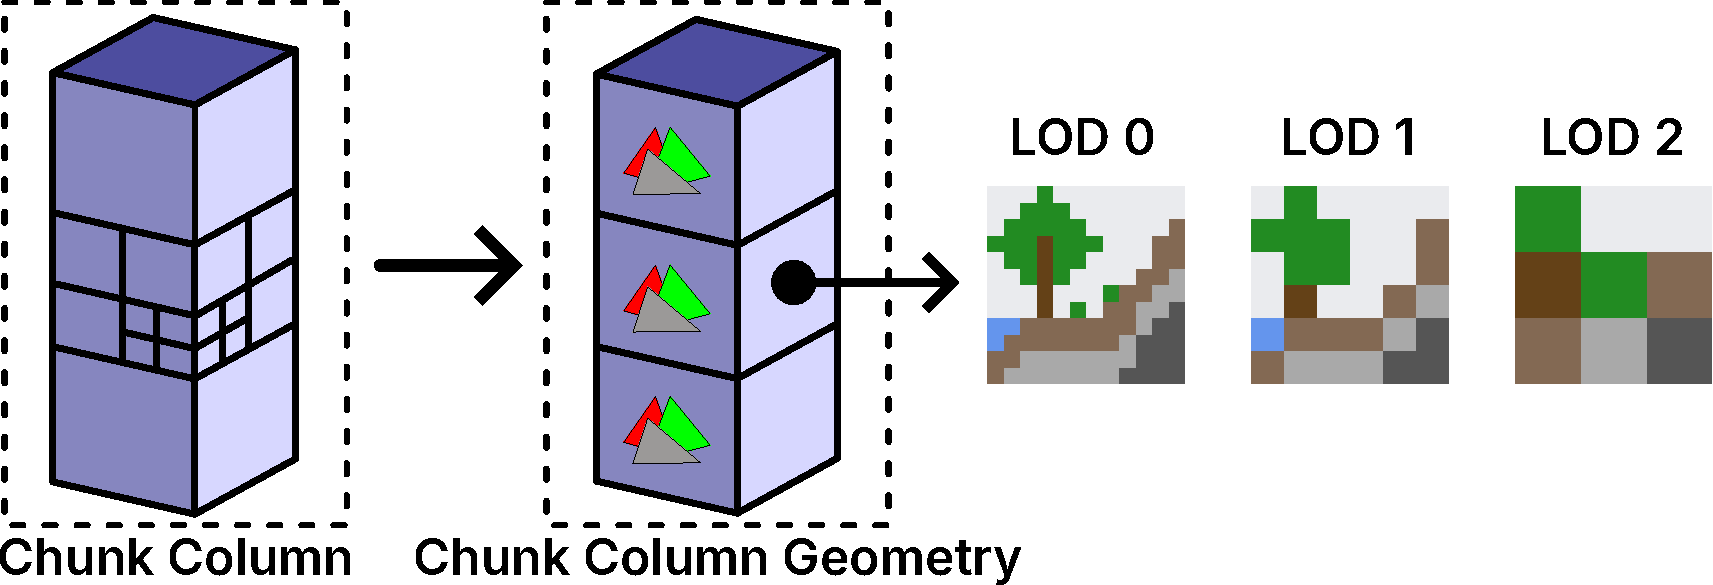
\includegraphics[width=0.75\textwidth]{obrazky-figures/geometry_visualization.pdf}
    \caption[Geometry Extraction]{Geometry extraction process including levels of detail.}
    \label{fig:geometry_visualization}
\end{figure}

\subsection{Geometry Extraction Dependencies}

Before a~specified Chunk Column can be processed, both it and its 4 neighbors must be fully voxelized. The reason is that the geometry extraction process is highly optimized to produce only visible faces. Thus, in order to generate geometry at the vertical boundaries of a~Chunk Column, it is required to have access to its neighbors.

Access to those neighbors is also optimized through an interconnected column network, so that a~neighboring column can be obtained directly from the current one.

\subsection{Geometry Extraction Process}

The generator processes chunks of Chunk Columns to extract their geometry and form Chunk Column Geometry structures with three LODs. These structures are visualized in Fig.~\ref{fig:geometry_structures}. The sizes of the voxel space that each LOD represents are shown in Tab.~\ref{tab:lod_levels}. The generator always generates geometry for all LODs at once, so the display process can switch between LODs quickly without waiting for the geometry of a~different LOD to be generated.

\begin{table}[]
\centering
\begin{tabular}{ccc}
\textbf{LOD0} & \textbf{LOD1} & \textbf{LOD2} \\ \hline
$1 \times 1 \times 1$   & $4 \times 4 \times 4$   & $8 \times 8 \times 8$   \\
\end{tabular}
\caption[LOD table]{Levels of detail and the sizes of voxel space they represent. In the smallest voxel units ($1/16$~m).}
\label{tab:lod_levels}
\end{table}

The generator follows the principles of cubical geometry extraction discussed in Section~\ref{ivr_rendering_voxels} and uses both naive geometry extraction and the optimized greedy meshing algorithm.

There are three categories of voxels from the perspective of the geometry generation process. These are air voxels, water voxels, and all other voxels representing solids. Only voxel faces that are at the transition between air and other voxel types are required. But as the visualization of the world utilizes various effects for water voxels, such as translucency and waves. The generation must be divided into independent extraction of water and solid geometry.

If a~chunk is detected to be entirely composed of air voxels, it is skipped and returned with no geometry. Further generation of a~chunk is also skipped if its first level of detail contains no geometry, as lower quality LODs would be empty as well.

\begin{figure}[b]
    \centering
    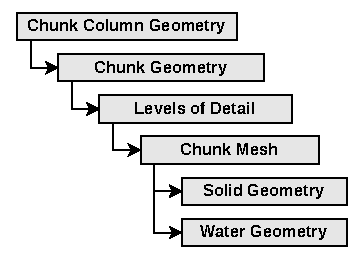
\includegraphics[width=0.35\textwidth]{obrazky-figures/geometry_structures.pdf}
    \caption[Chunk Column Geometry]{Internal structures for storing Chunk Column geometry information.}
    \label{fig:geometry_structures}
\end{figure}

\subsection{Specifics of Levels of Detail}

The small vegetation is generated only in the highest quality LOD. For this, there are two reasons. Firstly, the columns far from the camera can be further optimized. And secondly, the second LOD level is also used for the collision surfaces of the world physics layer, which enable character movement. If these contained the geometry of the small vegetation, the world would be practically non-traversable.

However, this also requires specific voxel types to filter out small vegetation. In the case of water plants, there are even more issues. As with lower-quality LODs, areas with many water plants would be sampled as plant voxels, which would not produce any faces, leaving holes in the water surfaces. To overcome this issue, a~specific category of submerged plant voxels is used. These allow for LOD-specific filtering during the geometry extraction process.

The implementation does not specifically handle the transitions between different LODs. Thus, it is possible to occasionally see missing faces at these positions.

\subsection{Compression of Geometry Data}

To reduce the memory cost of the stored geometry cache, the geometry is internally compacted. Firstly, vertex indices are used to reduce the number of vertices required to store a~single face from $6$ to only $4$. Then the normals and UV coordinates are compacted into a~single entry per face since they do not change across the four face vertices. The normals and UV coordinates are then expanded in the World Display layer to follow the format expected by the Godot Engine.

\subsection{Solid Geometry Extraction}

The geometry of solid voxel faces is extracted using the greedy meshing algorithm, which dramatically simplifies the generated geometry. The only solid voxel faces that are extracted are those that are at the transition between solids and air, as well as between solids and water. The greedy meshing algorithm uses voxel masks for the slices to reduce the number of queries to the voxel storage structures.

\subsection{Water Geometry Extraction}

The extraction of water faces does not utilize the greedy meshing algorithm. The reason is that the wave effect of the water requires all the sub-face vertices to be present. Otherwise, the water surface will be disconnected, jagged, and broken. Thus, the naive approach to cubical surface extraction is used. Water faces are generated only at the transitions between water and air voxels.

The water faces do not use UV coordinates to access the color atlas, as they form their own mesh and use a~custom shader material, which is further discussed in Section~\ref{world_display_layer}.


\section{World Display Layer}\label{world_display_layer}

The goal of the World Display layer is to visualize the generated column geometry in the Godot Engine and manage collision layers so the character can move through the world. As shown in Fig.~\ref{fig:world_display_service}, this layer serves as a~communication bridge between the hierarchical chunk system and the Godot Engine. Tasks defining which columns of the world should be displayed at which LOD and which should be completely unloaded are supplied to it by the Game Manager, as with other layers of the hierarchical system. But this layer does not process them in parallel or via its own threads. Instead, it uses the main thread of the engine, as support for multiple threads that are handling rendering-related tasks is still experimental in the Godot Engine\footnote{Discussed at:~\href{https://docs.godotengine.org/en/stable/tutorials/performance/thread_safe_apis.html}{\texttt{docs.godotengine.org/en/stable/tutorials/performance/thread\_safe\_apis.html}}}. 

\begin{figure}[t]
    \centering
    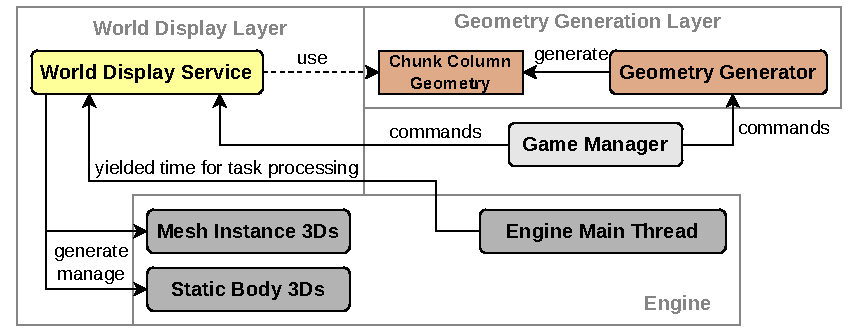
\includegraphics[width=0.775\textwidth]{obrazky-figures/world_display_service.pdf}
    \caption[World Display Layer]{Detailed World Display layer architecture diagram.}
    \label{fig:world_display_service}
\end{figure}

\subsection{Application of Geometry to the Engine}

The main thread of the Godot Engine periodically invokes functions in the World Display Service to unload inactive columns, visualize new ones, or update them at different LODs. Unloading of inactive columns always removes all scheduled columns. However, application of new geometry and column updates is a~performance-intensive process that stalls the main thread, as the engine must process the supplied geometry data. Thus, each invocation processes only up to two column updates.

Each chunk of the Chunk Column geometry structure has its geometry data of both water and solid surfaces expanded into a~form expected by the engine. This form is then used to create a~single \texttt{MeshInstance3D} node for each of those chunks, containing both mentioned surfaces. This node is then positioned in the engine scene so that it is displayed.

\subsection{Application of Collision Layers to the Engine}

It is also necessary to instantiate collision layers in the scene so that the character can move on the surface. As only a~small area around the character requires active collisions, the area defined by the highest quality level should be sufficient.

When the chunks of columns with LOD0 are managed, \texttt{StaticBody3D} nodes are instantiated in the engine from the chunk geometry of LOD1 quality level and placed in the same positions as the mesh instances. The LOD1 geometry is chosen because it is simplified and excludes small vegetation. Thus, allowing the character to move freely.

\subsection{Demo Visuals and Custom Shaders}

The surfaces with water and solid voxels utilize three Godot materials with two custom shaders. The surfaces of solid voxels use two different materials, depending on their viewed LOD quality level. Chunks displayed at the highest quality level use material with a~custom fragment shader that adds per-voxel color variance. It reconstructs the voxel grid of the smallest voxel size, using the positions of the vertices in world space. Then it uses these reconstructed positions to generate deterministic (hash-based) random values that modify the voxel colors from a~color atlas. Solid voxel surfaces at other quality levels use a~color atlas directly.

Water surfaces use material with a~custom shader as well. This shader uses values from a~precomputed noise texture to simulate simple animated waves by modifying the vertices' vertical positions. In the fragment shader, it attempts a~similar effect to the variance effect used for the solid surfaces, but animated. It uses two more precomputed noise textures, whose values are blended and modify the default color of the water surface.

The rest of the rendering process is done entirely by the engine. The project uses only two light sources -- a~sun represented by Godot \texttt{DirectionalLight3D} that follows the player through the world scene. It also supports a~very basic toggleable sun cycle. In which the sun moves around the horizon with changing light intensity. The second light is a~toggleable torch-like light source represented by Godot \texttt{OmniLight3D}, which is always next to the camera to illuminate the caves.

The project then uses a~Godot \texttt{WorldEnvironment} node, which, together with the lights, allows for shadows, global illumination via SDFGI (signed distance field global illumination), screen-space ambient occlusion, screen-space indirect lighting, and depth-based fog. The demo offers a~basic configuration screen for these effects, along with rendering distances, upscaling, and more.

\subsection{Support for Large Worlds in Terms of Rendering and Physics}

The engine internally uses floating-point numbers for rendering and physics, whose precision decreases with increasing distance from the world origin, as small details cannot be represented accurately at greater distances. In the case of the default 32-bit floating point numbers, the maximum recommended distance\footnote{Docs:~\href{https://docs.godotengine.org/en/stable/tutorials/physics/large_world_coordinates.html}{\texttt{docs.godotengine.org/en/stable/tutorials/physics/large\_world\_coordinates.html}}} from the world origin is around $4$--$8$~km. However, this demo aims to support significantly larger worlds.

There are many techniques that can be used to overcome this issue~\cite{large_world_support}. However, this demo uses a~very simple origin-shifting technique. The world is covered by a~grid of $512$ by $512$ meter cells, each denoting a~specific shifting offset. The character and all mesh and collision instances store their real-world position either with integers or, if a~decimal part is required, with 64-bit floating point numbers. Their position in the engine scene is then defined by applying the shifting offset to their real positions and is always around the world origin. When the character camera's real-world position crosses into a~different cell. A new shifting offset is used to reposition all objects back to the world origin.


\section{Implementation Details of Other Demo Features}

This section covers other notable implementation details, including the maximum supported environment size, environment editing, storage solutions, and world generation configuration options.

\subsection{World Size Limits}

The configured maximum distance of the camera from the world origin is $\pm$ \numprint{1000000}~m in each horizontal axis. Thus, a~single world covers \numprint{4000000}~$\text{km}^{\text{2}}$. These limits are placed at a~safe distance from areas that could pose issues. A large part of the implementation uses integer coordinates that allow for further continuation. However, at greater distances, the terrain starts to distort. Due to time constraints, these limits were chosen as a~safe compromise. It seems that at least some of these errors are due to floating-point precision issues in the internal noise functions, but it is possible that there are implementation errors in the demo as well.

\subsection{User-Based Voxel Editing}

User-based voxel editing is implemented with the help of ray casting into the Voxel Storage with the RLV algorithm (see Section~\ref{rlv}). Rays are cast through the voxel space from the center of the character camera, traversing it based on the selected voxel size for editing. The ray stops when it reaches non-air voxels or when a~configured maximum distance is traversed. In the first case, the voxel space of the selected size is edited. If the user is deleting voxels, then the voxel space is replaced with air voxels at the found positions. If~the user is placing voxels, then the selected voxel type is placed at the previous position.

The geometry of the affected chunk and its $6$~neighbors ($4$~horizontal and $2$~vertical) must then be regenerated in the Geometry Generation layer as a~special, high-priority task and reapplied in the World Display layer.

\subsection{Permanent Storage and Worlds}

The demo permanently stores application settings and data for the worlds it creates. Each world is stored with its configuration, the character's last position, and the user's voxel editing operations. The last is implemented trivially. Each column edited by the user appears in an index file of edited columns, along with its own file that contains a~list of all the user's editing operations in the order they were performed. The editing operations are stored instantly when the user performs them. When these columns are generated again, these operations are reapplied one by one. This simple implementation avoids storing all visited sections of the world. But if the user keeps editing the same voxels repeatedly, all these operations are retained and must be applied to reach the final state.

\subsection{Configuration of the World Generator}

World generation can be configured during world creation via a~GUI. It has several presets and supports a~detailed configuration of the generation process parameters. The supported parameters include seed, terrain height and type, threshold configuration for biome classification, cave and water system parameters, and more. Support for configuring voxel models is not implemented.


%%%%%%%%%%%%%%%%%%%%%%%%%%%%%%
% Results Analysis
%%%%%%%%%%%%%%%%%%%%%%%%%%%%%%
\chapter{Results Analysis}~\label{testing-showcase}

This chapter provides an analysis of the achieved results, compares the properties of the generated environments and demo capabilities to other game titles in the genre of sandbox voxel games, and discusses the performance of the implemented demo.

\section{Showcase of Generator Capabilities}

The procedural generator can create diverse worlds that resemble the properties of natural environments. The world features dynamic terrain with mountains, valleys, caves, and plateaus, naturally inspired water features, and biomes that form dry areas, snow-covered mountains, as well as forests and meadows at different stages of growth.

The generator is also highly configurable with detailed parameters and predefined presets. The main 32-bit seed value initializes PRNGs and procedural noise functions, allowing the creation of up to $2^{32}$ unique worlds, which are further specialized by other parameters, producing even more unique worlds in total.

However, there are still many areas open to improvement. Ranging from better terrain generation, which still feels unnatural due to the apparent use of procedural noise, to the overall diversity of the biomes, vegetation, and decoration models. Possible additions could include biomes such as swamps, wind-swept and rocky areas in highlands and mountains, as well as sub-biomes of the existing ones.

It would be beneficial to study in detail the wide range of natural terrains, realistic habitats, and plants, and to develop a~truly realistic generator of natural environments. 

\subsection{Showcase of the Default Preset}

The visual results of a~world generated with the default preset and seed of value $5000$ is shown in Fig.~\ref{fig:default_preset}. The collage of images visualizes the diversity of environments the generator can create. Note the overall diversity of the generated environments and the effects of water abundance (and its absence) on the generated biomes and placed vegetation.

\begin{figure}[t]
    \centering
    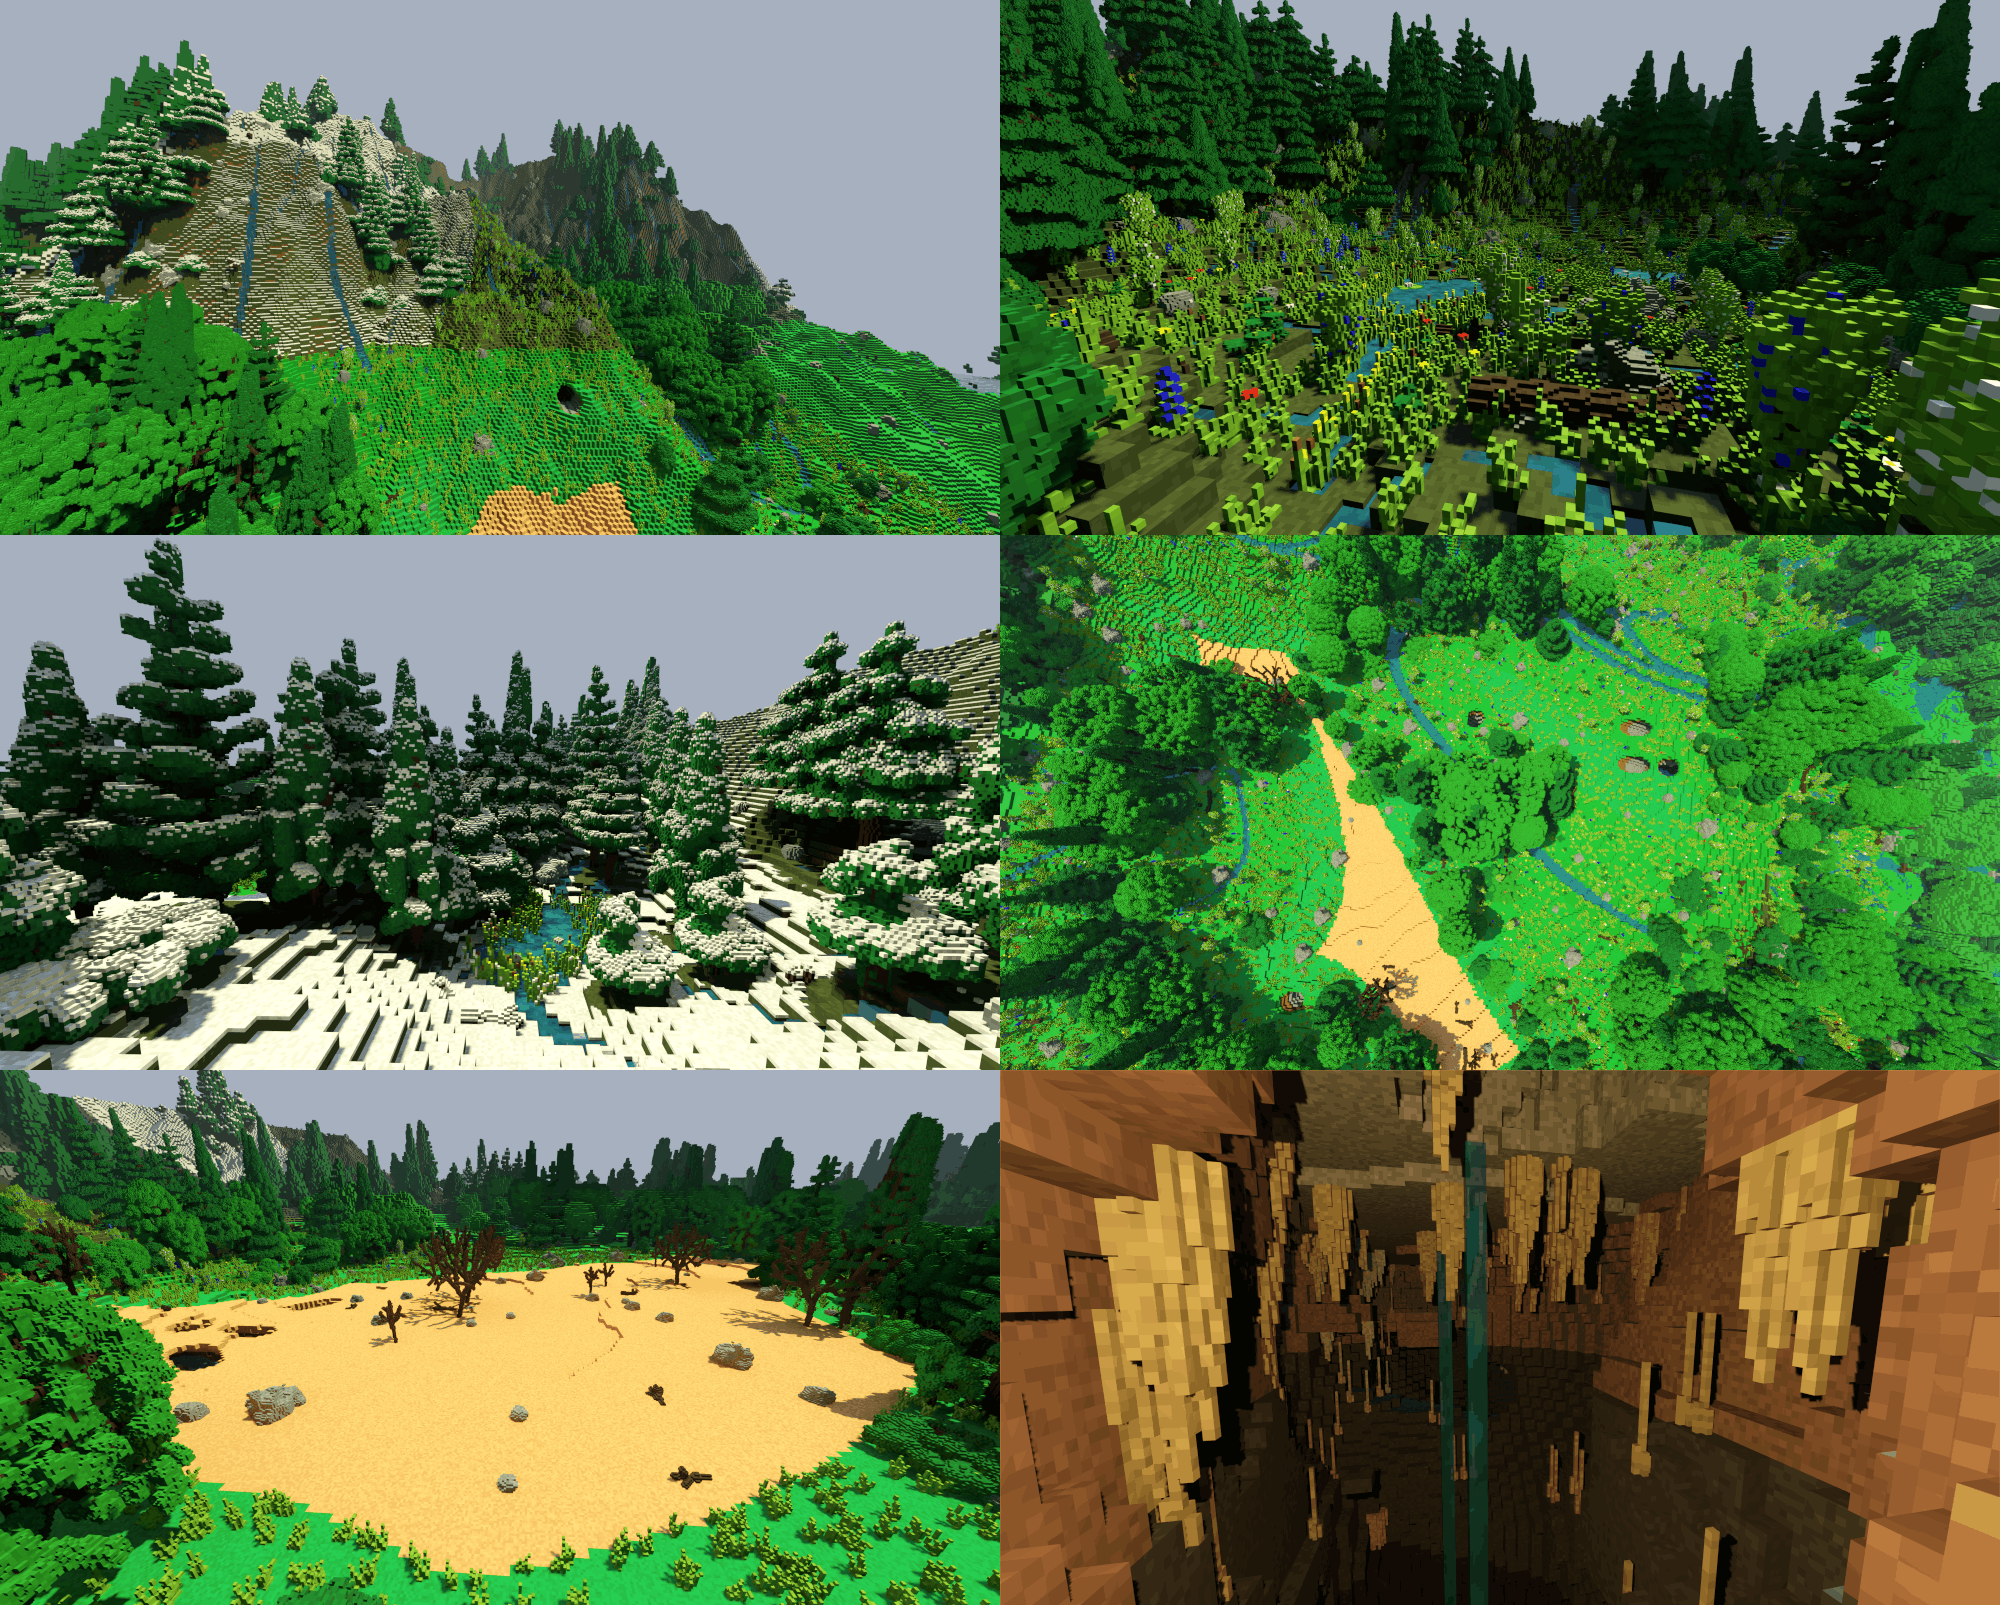
\includegraphics[width=1.0\textwidth]{obrazky-figures/results_normal.png}
    \caption[Results of Default Preset]{Visualization of the results of the default preset, including mountain ranges, lush vegetation, snow-covered areas, as well as deserts and underground caves.}
    \label{fig:default_preset}
\end{figure}

\subsection{Showcase of Other Presets}

The visualization of 6 additional configuration presets included in the demo is shown in Fig.~\ref{fig:other_presets}. All these presets use the same default seed value of $5000$ and show the configuration capabilities of the implemented demo.

\begin{figure}[t]
    \centering
    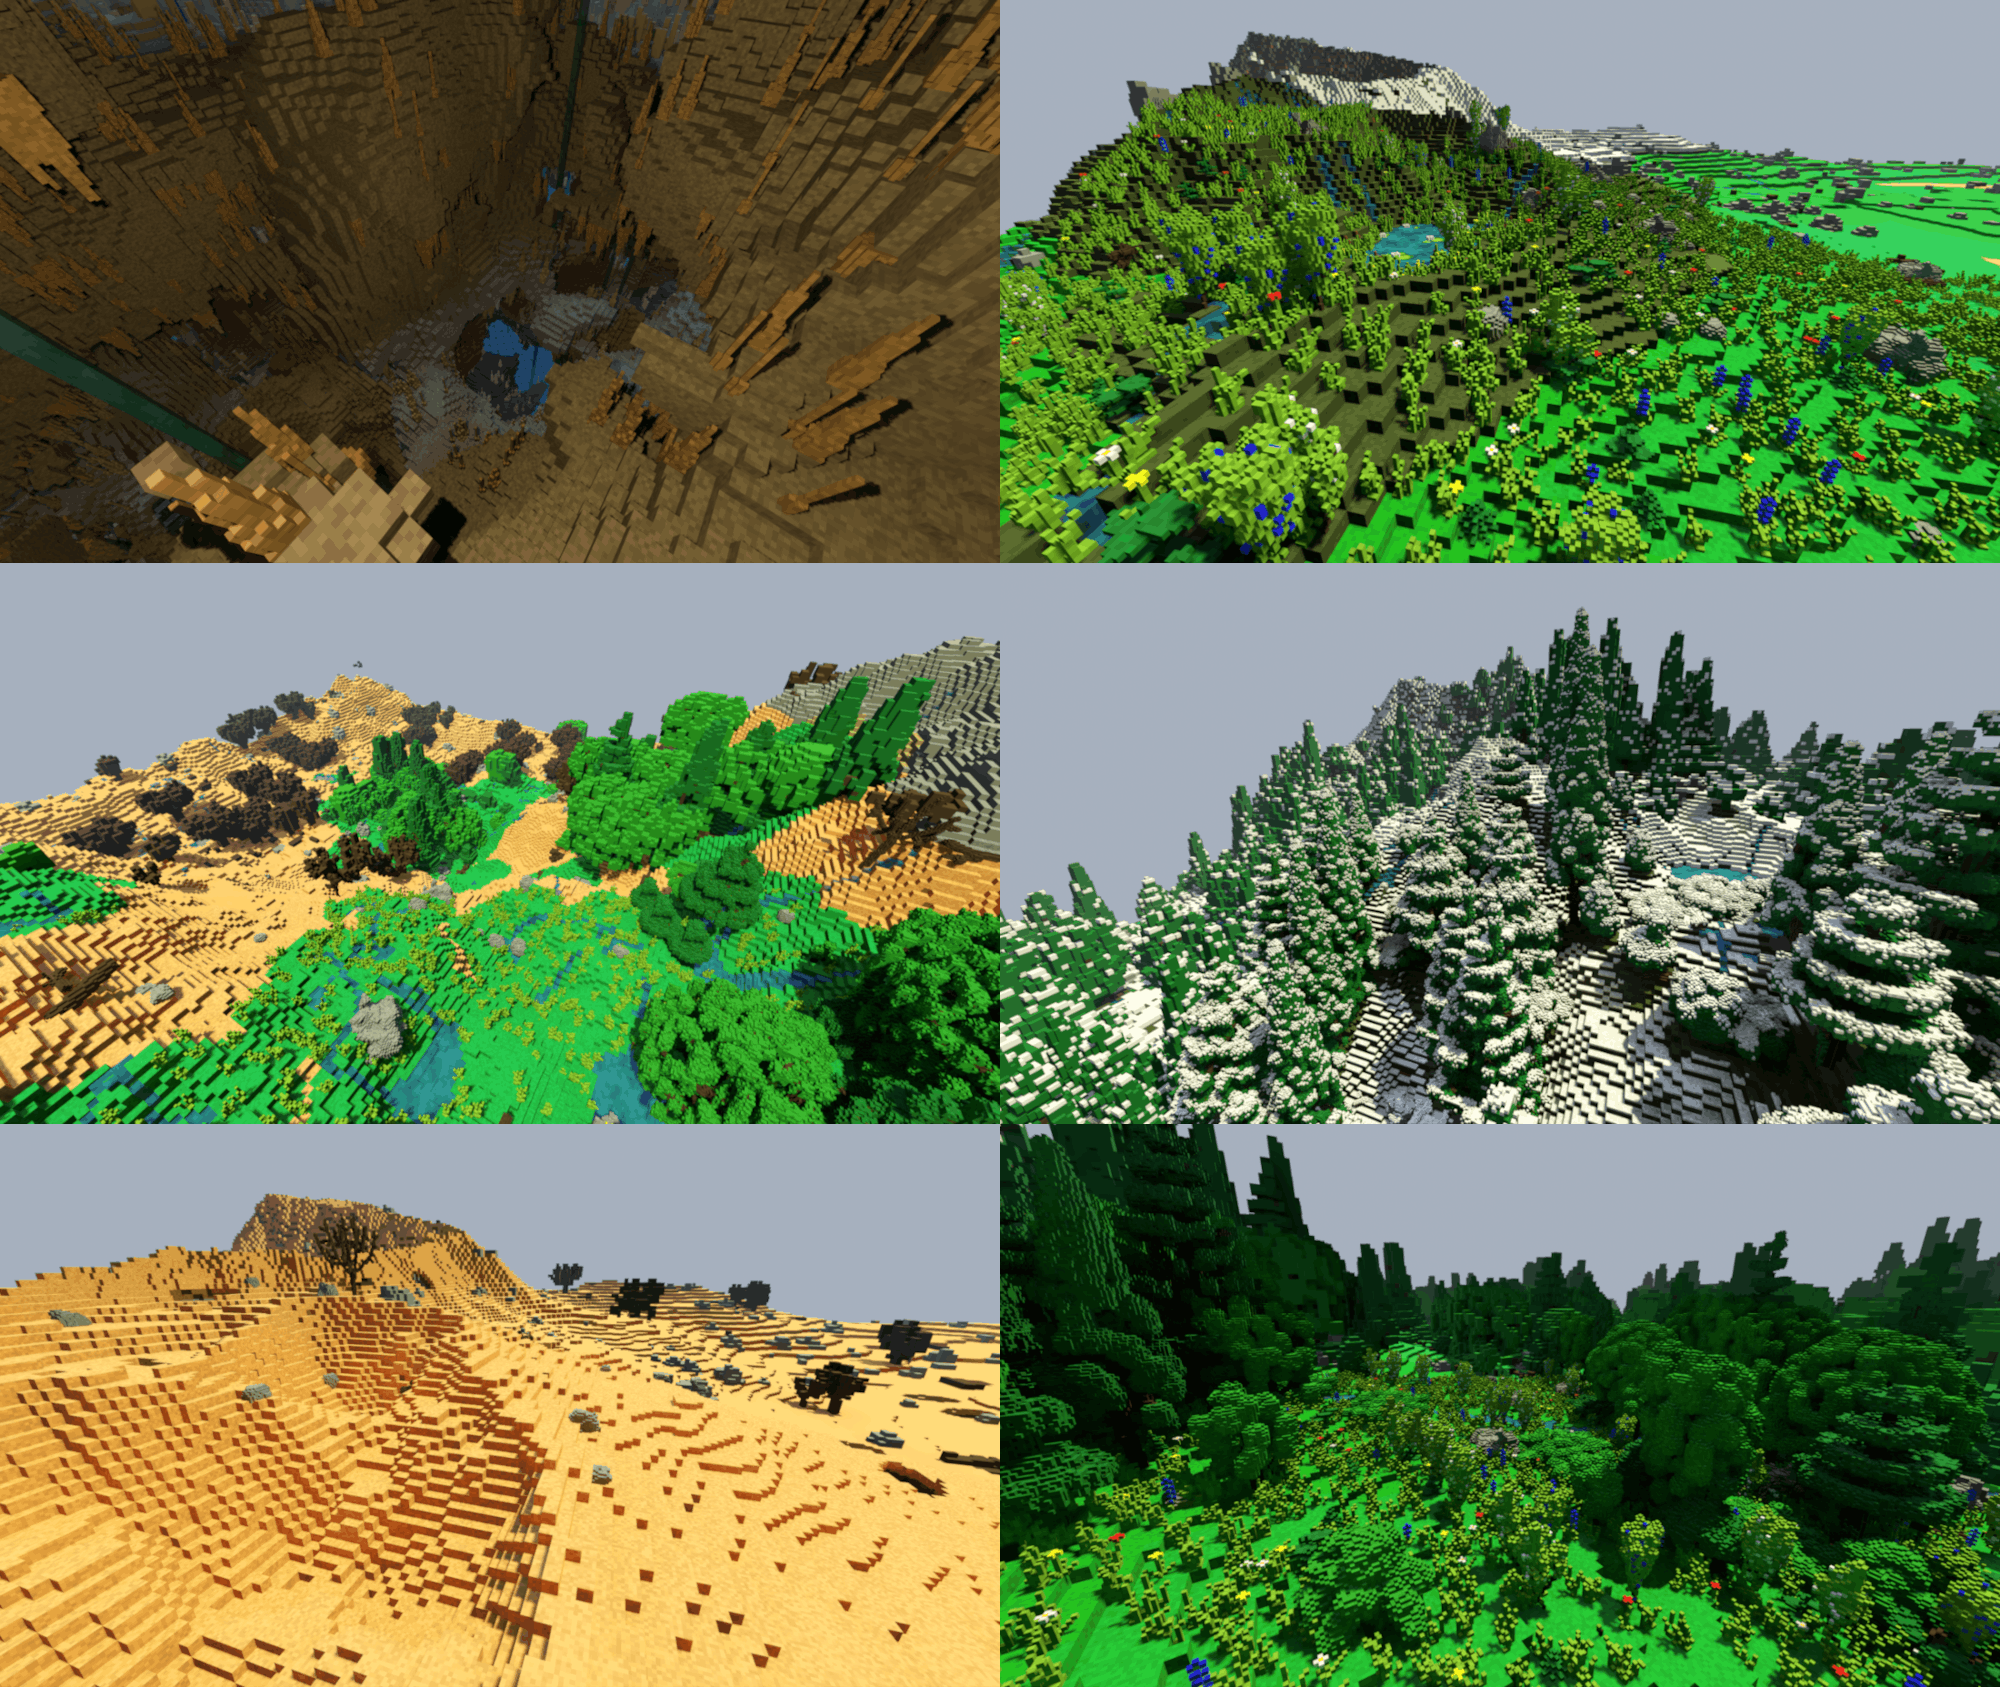
\includegraphics[width=1.0\textwidth]{obrazky-figures/results_other.png}
    \caption[Results of Other Presets]{Visualization of the results of other presets. From left to right and top to bottom. Deep caves, without trees, dry land, snowy world, desert, and lush vegetation.}
    \label{fig:other_presets}
\end{figure}

\section{Comparison with Other Game Titles}

In contrast to this demo, existing sandbox voxel games such as Minecraft, Lay of the Land, or Hytale feature significantly more diverse environments. Especially when it comes to the variety of their biomes and structures, which often serve as important gameplay elements. This demo focuses only on generating natural landscapes with dense vegetation, without any non-natural elements, as discussed in the goals of the world generator in Chapter~\ref{world-gen-design}.

It also features limited gameplay elements that focus on exploring the generated worlds and altering them. This demo uses high voxel detail, similar to the game Lay of the Land, which allows vegetation and decorations to be represented by small voxels and opens up gameplay possibilities that are not possible in games such as Minecraft, due to their large voxel sizes. This way, the demo bridges the gap between these types of games.

\section{Performance Analysis}

The implemented demo is quite performance-heavy in terms of memory usage and CPU and GPU computation time, even though several optimizations were implemented. The following sections analyze the demo's performance properties. The results were obtained with Godot Engine version 4.6.2 and the .NET SDK version 10, with runtime optimizations enabled. The reference device uses Fedora 43 Workstation Edition, kernel version 6.19.12, Mesa version 25.3.6, 48 GB of dual-channel DDR4 memory, a~Ryzen 9 5900XT CPU, and a~Radeon RX 7700XT GPU.

\subsection{Memory Utilization}

The application was tested with several different view distances with the default world preset and seed value of $5000$. For each view distance, the values were measured after all tasks were completed. The results are shown in Tab.~\ref{tab:memory_usage}.

\begin{table}[]
\centering
\begin{tabular}{l|rrrr}
 & Very Low & Low & Medium & High \\ \hline
Geometry Cache                 & 370                                   & 894                              & \numprint{1870}        & \numprint{5600}      \\
Voxel Storage                  & 348                                   & 794                              & \numprint{1380}        & \numprint{3400}      \\
World Regions                  & 235                                   & 235                              & 235                                 & 235                               \\
.NET Total                     & \numprint{1260}                      & \numprint{2280}     & \numprint{4060}        & \numprint{11910}     \\
Total Memory                   & \numprint{1750}         & \numprint{2790}     & \numprint{4570}        & \numprint{12350}    
\end{tabular}
\caption[Memory Usage Testing]{Memory usage of the application at different view distances  (from very low to high) in megabytes. Measured at the world center of default preset and seed value of $5000$ after all tasks are finished.}
\label{tab:memory_usage}
\end{table}

It can be seen that memory usage varies significantly with the configured view distance, as higher view distances require more columns to be voxelized and have their geometry generated. On the other hand, the memory used by active regions stays roughly the same. The application should scale well across devices with varying amounts of usable memory.

Memory requirements depend heavily on the environments visited and the world generator parameters. Environments with mountain ranges, deep caves, and dense vegetation can increase it, as do world generator parameters that configure these features. In real-case scenarios, when the user moves through the environment, the memory usage will be slightly higher, as the region and column buffers will be saturated.

\subsection{Parallel Processing}

The implementation is highly parallelized, with each of the hierarchical levels utilizing up to a~configured number of threads, which are dependent on the total thread count available on the CPU, as is shown in Eq.~\ref{eq:thread_assignment}, where $t$~denotes the total number of threads available on the CPU, $t_m$~specifies model generator threads, $t_w$~world generator threads, $t_v$~voxelization threads, and $t_g$~the threads used by the geometry generator. These numbers were selected to leverage the advantages of high-core CPUs without over-utilizing them. Maximum utilization showed lower overall performance, possibly due to high allocation rates, decreased CPU frequencies, runtime limitations, and locking of shared resources.

\begin{equation}\label{eq:thread_assignment}
    \begin{aligned}
        t_m &= \text{max}\left(1, t/2\right) \\
        t_w &= \text{max}\left(1, t/6\right) \\
        t_v &= \text{max}\left(1, t/3\right) \\
        t_g &= \text{max}\left(1, t/1.3\right) \\
    \end{aligned}
\end{equation}

\subsection{Computational Cost of the Hierarchical Layers}

The comparison of the computational cost of the layers is based on the total time required to complete all tasks scheduled at the world startup for the default world preset and seed value of $5000$. Calculated as the combined thread time spent on task processing. To better capture the computational cost of each layer, this test is run at 4 different view distances.

The model generator runs before the chunk system starts up and takes approximately $2.87$ seconds or $21.8$ seconds of combined thread time to generate all models on the reference device. Then starts the hierarchical chunk system. The combined thread time required to complete all tasks across all layers is visible in Tab.~\ref{tab:comp_cost}. All these values are averages across three runs.

\begin{table}[]
\centering
\begin{tabular}{l|rr|rr|rr|rr}
& \multicolumn{2}{c|}{Very Low}                 & \multicolumn{2}{c|}{Low}                             & \multicolumn{2}{c|}{Medium}                           & \multicolumn{2}{c}{High} \\
& \multicolumn{1}{c}{Time} & \multicolumn{1}{c|}{\%} & \multicolumn{1}{c}{Time} & \multicolumn{1}{c|}{\%} & \multicolumn{1}{c}{Time} & \multicolumn{1}{c|}{\%} & \multicolumn{1}{c}{Time} & \multicolumn{1}{c}{\%} \\ \hline
World Generation    & \multicolumn{1}{r}{\numprint{57.95}}                  & 25                               & \multicolumn{1}{r}{\numprint{58.6}}                  & 12                               & \multicolumn{1}{r}{\numprint{63.83}}                  & 6                                & \multicolumn{1}{r}{\numprint{60.69}}                  & 2                                \\
Voxel Generation    & \multicolumn{1}{r}{\numprint{17.49}}                  & 8                                & \multicolumn{1}{r}{\numprint{37.56}}                  & 7                                & \multicolumn{1}{r}{\numprint{63.6}}                  & 7                                & \multicolumn{1}{r}{\numprint{160.46}}                 & 6                                \\
Geometry Generation & \multicolumn{1}{r}{\numprint{156.46}}                 & 67                               & \multicolumn{1}{r}{\numprint{413.43}}                 & 81                               & \multicolumn{1}{r}{\numprint{848.64}}                 & 87                               & \multicolumn{1}{r}{\numprint{2443.37}}                & 92                               \\
\end{tabular}
\caption[Computational Cost of Chunk System]{Combined thread times in seconds it takes to finish all tasks scheduled for the three most performance-heavy layers of the hierarchical chunk system at the startup of the same world with different render distances (from very low to high).}
\label{tab:comp_cost}
\end{table}

The combined thread time required to generate the necessary World Regions remains roughly the same, as with memory requirements. It can be seen that by far the most processing time is spent generating geometry, largely due to the task's complexity and the greedy meshing algorithm. Compared to it, the Voxel Generation and World Generation layers have a~very low computational cost. The best target for demo optimizations would thus be the Geometry Generation layer. It might be even better to switch to visualization via surface ray casting (discussed in Section~\ref{dvr}). This would also eliminate the need for a~geometry cache, but the voxel data would have to be stored in VRAM as well.

Generally, the demo should be able to run on CPUs significantly less powerful than the tested Ryzen 9 5900XT, especially at lower render distances when less work is required.

\subsection{Application of Geometry in the Engine}

The geometry application process in the World Display layer runs on the engine's main thread and thus is not part of the analysis in the previous section. However, it is also the place with the most noticeable performance issues, as even a~portioned geometry application, which applies at most 2 column updates per frame, still causes main-thread stalls and perceivable stuttering. Using a~single-column update per frame, or even applying only a~few chunks at a~time, also does not fix these issues, as the system cannot keep up with the required changes.

The solution would be to implement the geometry application with multi-threading, but support for this is still experimental in the Godot Engine. Another option would be to switch to surface ray casting, implemented on the GPU. However, synchronizing voxel storage between RAM and VRAM could also pose issues.

\subsection{Rendering Performance}

The average frame rates achieved by the demo on the reference device across different visual configuration options and render distances are shown in Tab.~\ref{tab:framerates}. These values were obtained by moving at the surface and through caves around the world center. The tested world used the default preset and seed $5000$. During testing, noticeable stuttering was observed at medium and high render distances.

\begin{table}[!h]
\centering
\begin{tabular}{l|rrrr}
    & Very Low & Low & Medium & High \\ \hline
All enabled, MSAA 2X & 296     & 239                               & 174                                  & 73 \\
All disabled, FSR 2.2 at 50\%          & \numprint{1233}                                   & 754                               & 444                                  & 170
\end{tabular}
\caption[Rendering Performance]{Average FPS of the demo with different configuration options and render distances (from very low to high). Tested on the reference device at $1920\times1080$ resolution.}
\label{tab:framerates}
\end{table}

%%%%%%%%%%%%%%%%%%%%%%%%%%%%%%
% Conclusion
%%%%%%%%%%%%%%%%%%%%%%%%%%%%%%
\chapter{Conclusion}\label{conclusion}

The goal of this thesis was to study the use of procedural generation methods and voxel environments in games and design, and implement a~procedural voxel map generator in the form of a~game demo.

The use of procedural generation methods and voxel environments in game development was studied primarily in the context of sandbox voxel games, such as Minecraft and Lay of the Land, and focused on the generation of naturally inspired world environments. Then, a~procedural world generator for voxel game maps was designed to generate natural environments with diverse terrains, water elements, biomes, vegetation, and other structures, such as underground caves and decorations. This generator was then implemented in a~fully procedurally generated sandbox voxel game demo that features pseudo-infinite worlds and allows their exploration and editing.

The demo features a~high level of voxel detail somewhere between Minecraft and Lay of the Land. It can create diverse environments, including mountains, plateaus, valleys, and underground caves with decorations. The surface is covered with rivers and lakes that follow the terrain's properties, and biomes with vegetation and decorations that reflect water availability and terrain height. The resulting environments range from snow-covered mountains and hills, through arid plains, to meadows and forests with lush vegetation. The demo also supports multiple worlds, configurable world generation, teleportation, and more. 

The resulting demo is capable of creating diverse and detailed voxel environments, it delivers acceptable performance given its level of voxel detail, and it supports a~wide range of configuration options. Its greatest strength is the naturally inspired generation of meadows and forests. It could be used for the development of fully featured sandbox voxel games or for educational purposes.

Areas for improvement include further optimizations, fixing stuttering and missing faces at transitions between levels of detail, and improving the world generator to provide more detailed, real-life-accurate environments with realistic plants, terrain formations, and a~larger set of biomes. Issues with stuttering, missing faces, and possible optimizations could potentially be improved with the switch to rendering with surface ray casting.
